%
% Template Laporan Skripsi/Thesis Universitas Indonesia
%
% @author  Ichlasul Affan, Azhar Kurnia
% @version 2.1.3
%
% Dokumen ini dibuat berdasarkan standar IEEE dalam membuat class untuk
% LaTeX dan konfigurasi LaTeX yang digunakan Fahrurrozi Rahman ketika
% membuat laporan skripsi, yang kemudian diadaptasi oleh Andreas Febrian dan
% Lia Sadita untuk template skripsi tahun 2010.
% Konfigurasi template sebelumnya telah disesuaikan dengan
% aturan penulisan thesis yang dikeluarkan UI pada tahun 2017.
%

%
% Tipe dokumen adalah report dengan satu kolom.
%
\documentclass[12pt, a4paper, onecolumn, twoside, final]{report}
\raggedbottom

% Load konfigurasi LaTeX untuk tipe laporan thesis
\usepackage{_internals/uithesis}
%


% Load konfigurasi khusus untuk laporan yang sedang dibuat
%-----------------------------------------------------------------------------%
% Judul Dokumen
%-----------------------------------------------------------------------------%
%
% Judul laporan.
\def\judul{\textit{Re-ranker} Berbasis Fitur untuk \textit{Information Retrieval} pada Domain Legal}
%
% Tulis kembali judul laporan namun dengan bahasa Ingris
\def\judulInggris{Feature Based Re-Ranker for Legal Domain Retrieval}


%-----------------------------------------------------------------------------%
% Tipe Dokumen
%-----------------------------------------------------------------------------%
%
% Tipe laporan, dapat berisi: Laporan Kerja Praktik, Kampus Merdeka, Skripsi, Tugas Akhir, Thesis, atau Disertasi
\def\type{Skripsi}
%
% Nama jalur Kampus Merdeka (hanya perlu diisi jika tipe laporan adalah Kampus Merdeka
% Contoh isian (khusus Fasilkom): Studi Independen, Magang Mitra, Magang BUMN, Bangkit, Apple Academy, BYOC
\def\kampusMerdekaType{}
% Jika ada perwakilan mitra, isi dengan jabatan perwakilan mitra tersebut
% (misal: Cohort Manager)
% Kosongkan jika tidak ada perwakilan mitra
\def\partnerPosition{}
% Jika ada perwakilan mitra, isi dengan nama perusahaan atau nama program
% (misal: PT. Astra International, Bangkit Academy 2023)
% Kosongkan jika tidak ada perwakilan mitra
\def\partnerInstance{}
%
% Jenjang studi, dapat berisi: Diploma, Sarjana, Magister, atau Doktor
\def\jenjang{Sarjana}


%-----------------------------------------------------------------------------%
% Informasi Penulis
%-----------------------------------------------------------------------------%
%
% Tulis nama Anda
% Kosongkan penulisDua dan penulisTiga jika Anda melaksanakan tugas akhir/laporan secara individu
\def\penulisSatu{Kenneth Jonathan} % nama lengkap penulis pertama
\def\penulisDua{} % nama lengkap penulis kedua
\def\penulisTiga{} % nama lengkap penulis ketiga
%
% Tulis NPM Anda
% Kosongkan npmDua dan npmTiga jika Anda melaksanakan tugas akhir/laporan secara individu
\def\npmSatu{2006463364} % NPM penulis pertama
\def\npmDua{} % NPM penulis kedua
\def\npmTiga{} % NPM penulis ketiga
%
% Tulis Program Studi yang Anda ambil
% Kosongkan programDua dan programTiga jika Anda melaksanakan tugas akhir/laporan secara individu
\def\programSatu{Ilmu Komputer} % program studi penulis pertama
\def\programDua{} % program studi penulis kedua
\def\programTiga{} % program studi penulis ketiga
%
% Tulis Program Studi yang Anda ambil dalam bahasa inggris
% Kosongkan programDua dan programTiga jika Anda melaksanakan tugas akhir/laporan secara individu
\def\studyProgramSatu{Computer Science} % 1st author's study program
\def\studyProgramDua{} % 2nd author's study program
\def\studyProgramTiga{} % 3rd author's study program


%-----------------------------------------------------------------------------%
% Informasi Dosen Pembimbing & Penguji
%-----------------------------------------------------------------------------%
%
% Tuliskan pembimbing
% Untuk Kampus Merdeka: Tuliskan dosen PIC/pembimbing dari Fakultas Anda
\def\pembimbingSatu{Alfan Farizki Wicaksono, Ph.D.}
% S1 s.d. S3: Kosongkan jika tidak ada pembimbing kedua
% Untuk Kampus Merdeka: Tuliskan penanggung jawab/penyelia/mitra
%                       dari program Kampus Merdeka yang Anda ambil (jika ada)
\def\pembimbingDua{}
% S2 & S3: Kosongkan jika tidak ada pembimbing ketiga
\def\pembimbingTiga{}

%
% Tuliskan penguji
\def\pengujiSatu{Penguji Pertama Anda}
\def\pengujiDua{Penguji Kedua Anda}
% Kosongkan jika tidak ada penguji ketiga (umumnya penguji ketiga hanya ada untuk S2)
\def\pengujiTiga{}
% Kosongkan jika tidak ada penguji keempat, kelima, atau keenam (umumnya penguji > 3 hanya ada untuk S3)
\def\pengujiEmpat{}
\def\pengujiLima{}
\def\pengujiEnam{}


%-----------------------------------------------------------------------------%
% Informasi Lain (Asal Fakultas, Tanggal, dsb.)
%-----------------------------------------------------------------------------%
%
% Tuliskan Fakultas dimana penulis berada
\def\fakultas{Ilmu Komputer}
%
% Tuliskan bulan dan tahun publikasi laporan
\Var{\bulanTahun}{Juni 2024}
%
% Tuliskan gelar yang akan diperoleh dengan menyerahkan laporan ini
\def\gelar{Sarjana}
%
% Tuliskan tanggal pengesahan laporan, waktu dimana laporan diserahkan ke
% penguji/sekretariat
\def\tanggalSiapSidang{Tanggal Bulan Tahun}
%
% Tuliskan tanggal keputusan sidang dikeluarkan dan penulis dinyatakan
% lulus/tidak lulus
\def\tanggalLulus{Tanggal Bulan Tahun}


%-----------------------------------------------------------------------------%
% Judul Setiap Bab
%-----------------------------------------------------------------------------%
%
% Berikut ada judul-judul setiap bab.
% Silahkan diubah sesuai dengan kebutuhan.
%
\Var{\kataPengantar}{Kata Pengantar}
\Var{\babSatu}{Pendahuluan}
\Var{\babDua}{Studi Literatur}
\Var{\babTiga}{Metodologi}
\Var{\babEmpat}{Implementasi}
\Var{\babLima}{Eksperimen dan Analisis}
\Var{\babEnam}{Penutup}


%-----------------------------------------------------------------------------%
% Capitalized Variables
% Anda tidak perlu mengubah apapun di bagian ini
%-----------------------------------------------------------------------------%
\Var{\Judul}{\judul}
\Var{\Type}{\type}
\Var{\PenulisSatu}{\penulisSatu}
\Var{\PenulisDua}{\penulisDua}
\Var{\PenulisTiga}{\penulisTiga}
\Var{\Fakultas}{\fakultas}
\Var{\ProgramSatu}{\programSatu}
\Var{\ProgramDua}{\programDua}
\Var{\ProgramTiga}{\programTiga}



% Daftar pemenggalan suku kata dan istilah dalam LaTeX
%
% Hyphenation untuk Indonesia
%
% @author  Andreas Febrian
% @version 2.1.2
% @edit by Ichlasul Affan, Muhammad Aulia Adil Murtito
%
% Tambahkan cara pemenggalan kata-kata yang salah dipenggal secara otomatis
% oleh LaTeX. Jika kata tersebut dapat dipenggal dengan benar, maka tidak
% perlu ditambahkan dalam berkas ini. Tanda pemenggalan kata menggunakan
% tanda '-'; contoh:
% menarik
%   --> pemenggalan: me-na-rik
%


% Silakan ganti ke bahasa Inggris (\selectlanguage{english}) jika Anda merasa terlalu banyak kata bahasa Inggris yang pemenggalannya tidak benar.
%\selectlanguage{english}


\hyphenation{
    % alphabhet A
    a-na-li-sa a-tur a-tur-an
    a-pli-ka-si
    % alphabhet B
    bab ba-ngun-an
    be-be-ra-pa
    ber-ge-rak
    ber-ke-lan-jut-an
    ber-o-per-ra-si
    ber-pe-nga-ruh
    % alphabhet C
    ca-ri Com-po-nent-UML
    % alphabhet D
    di-da-pat-kan di-sim-pan di-pim-pin di-tam-bah-kan di-tem-pat-kan de-ngan da-e-rah di-ba-ngun di-gu-na-kan da-pat di-nya-ta-kan
    di-se-mat-kan di-sim-bol-kan di-pi-lih di-li-hat de-fi-ni-si di-de-fi-ni-si-kan di-mo-del-kan di-mi-li-ki di-re-a-li-sa-si-kan di-su-sun
    % alphabhet E
    eks-pli-sit e-ner-gi en-gi-neer en-gi-neer-ing eks-klu-sif ele-men
    % alphabhet F
    fa-si-li-tas
    % alphabhet G
    ga-bung-an ge-rak ge-ne-ral ge-ne-ra-li-sa-si
    % alphabhet H
    ha-lang-an
    % alphabhet I
    in-fra-struk-tur i-ni-si-a-si
    % alphabhet J
    % alphabhet K
    ke-hi-lang-an
    ke-ter-hu-bung-an
    ku-ning
    kua-li-tas ka-me-ra ke-mung-kin-an ke-se-pa-ham-an
    % alphabhet L
    ling-kung-an
    % alphabhet M
    ma-na-je-men me-neng-ah meng-a-da-kan me-mo-ni-tor
    me-mer-lu-kan me-mo-del-kan men-de-fi-ni-si-kan meng-ak-ses me-ne-mu-kan
    meng-a-tas-i me-mo-di-fi-ka-si me-mung-kin-kan me-nge-na-i me-ngi-rim-kan meng-i-zin-kan
    meng-u-bah meng-a-dap-ta-si me-nya-ta-kan me-nyim-pan me-res-trik-si mi-cro-ser-vi-ce mi-cro-ser-vi-ces mo-di-fi-ka-si mo-dul mo-dule
    meng-a-tur meng-a-rah-kan mi-lik meng-gu-na-kan me-ne-ri-ma me-nga-la-mi
    % alphabhet N
    nya-ta non-eks-klu-sif
    % alphabhet O
    o-pe-ra-si or-ga-ni-sa-si
    % alphabhet P
	pe-nye-rap-an
	pe-ngon-trol
    pe-mo-del-an
    pe-ran  pe-ran-an-nya
    pem-ba-ngun-an pre-si-den pe-me-rin-tah pe-mi-li-han prio-ri-tas peng-am-bil-an
    peng-ga-bung-an pe-nga-was-an pe-ngem-bang-an
    pe-nga-ruh pe-nge-lo-la pa-ra-lel-is-me per-hi-tung-an per-ma-sa-lah-an
    pen-ca-ri-an pen-ce-ta-kan peng-struk-tur-an pen-ting pen-ting-nya pe-ngu-ku-ran
    pre-sen-ta-si
    % alphabhet Q
    % alphabhet R
    ran-cang-an re-fe-ren-si re-pre-sen-ta-si
    % alphabhet S
    sub-bab si-mu-la-si sa-ngat ska-la-bi-li-tas
    stan-dar-di-sa-si
    % alphabhet T
    te-ngah
    ter-da-pat
    trans-for-ma-si
    % alphabhet U
    % alphabhet V
    va-li-da-si va-ri-an va-ri-a-si va-ri-a-bi-li-tas ve-ri-fi-ka-si
    % alphabhet W
    % alphabhet X
    % alphabhet Y
    % alphabhet Z
    % special
}

% Daftar istilah yang mungkin perlu ditandai
%
% @author  Andreas Febrian
% @version 1.00
%
% Mendaftar seluruh istilah yang mungkin akan perlu dijadikan
% italic atau bold pada setiap kemunculannya dalam dokumen.
%

\var{\license}{\f{Creative Common License 1.0 Generic}}
\var{\bslash}{$\setminus$}

% Italic Stuff
\newcommand{\ir}[1]{\textit{Information Retrieval}}
\newcommand{\reranker}[1]{\textit{re-ranker}}
\newcommand{\Reranker}[1]{\textit{Re-ranker}}
\newcommand{\sparse}[1]{\textit{sparse}}
\newcommand{\txt}[1]{\textit{text}}
\newcommand{\training}[1]{\textit{training}}
\newcommand{\testing}[1]{\textit{testing}}
\newcommand{\matching}[1]{\textit{matching}}
\newcommand{\alg}[1]{\textit{algorithm}}
\newcommand{\feature}[1]{\textit{feature}}
\newcommand{\extraction}[1]{\textit{extraction}}
\newcommand{\score}[1]{\textit{score}}
\newcommand{\contextual}[1]{\textit{contextual}}
\newcommand{\word}[1]{\textit{word}}
\newcommand{\embedding}[1]{\textit{embedding#1}}
\newcommand{\corpus}[1]{\textit{corpus}}
\newcommand{\heuristic}[1]{\textit{heuristic}}
\newcommand{\pipeline}[1]{\textit{pipeline}}
\newcommand{\reranking}[1]{\textit{re-ranking}}
\newcommand{\ml}[1]{\textit{machine learning}}
\newcommand{\query}[1]{\textit{query}}
\newcommand{\base}[1]{\textit{base}}
\newcommand{\retrieval}[1]{\textit{retrieval}}
\newcommand{\retriever}[1]{\textit{retriever}}
\newcommand{\cutoff}[1]{\textit{cut-off}}
\newcommand{\learning}[1]{\textit{learning}}
\newcommand{\ablation}[1]{\textit{ablation}}
\newcommand{\recall}[1]{\textit{recall}}
\newcommand{\precision}[1]{\textit{precision}}
\newcommand{\semantic}[1]{\textit{semantic}}
\newcommand{\similarity}[1]{\textit{similarity}}
\newcommand{\neural}[1]{\textit{neural}}
\newcommand{\network}[1]{\textit{network}}
\newcommand{\nn}[1]{\neural{} \network{}}
\newcommand{\incremental}[1]{\textit{incremental}}
\newcommand{\importance}[1]{\textit{importance}}
\newcommand{\task}[1]{\textit{task}}
\newcommand{\file}[1]{\textit{file}}
\newcommand{\error}[1]{\textit{error}}
\newcommand{\article}[1]{\textit{article}}
\newcommand{\cascade}[1]{\textit{cascade}}
\newcommand{\cascaded}[1]{\textit{cascaded}}
\newcommand{\parsing}[1]{\textit{parsing}}
\newcommand{\entail}[1]{\textit{entail}}
\newcommand{\weighting}[1]{\textit{weighting}}
\newcommand{\term}[1]{\textit{term}}
\newcommand{\token}[1]{\textit{token#1}}
\newcommand{\hs}[1]{\textit{hidden state#1}}
\newcommand{\hcf}[1]{\textit{hand-crafted features}}
\newcommand{\regex}[1]{\textit{regular expression}}
\newcommand{\ranking}[1]{\textit{ranking}}
\newcommand{\library}[1]{\textit{library}}
\newcommand{\baseline}[1]{\textit{baseline}}
\newcommand{\encoder}[1]{\textit{encoder}}
\newcommand{\decoder}[1]{\textit{decoder}}
\newcommand{\fcv}[1]{\textit{5-fold cross validation}}
\newcommand{\ltr}[1]{\textit{learning to rank}}
\newcommand{\paralegal}[1]{\textit{paralegal}}
\newcommand{\dataset}[1]{\textit{dataset}}

%% With Capitalization Stuff
\newcommand{\Base}[1]{\textit{Base}}
\newcommand{\Txt}[1]{\textit{Text}}
\newcommand{\Matching}[1]{\textit{Matching}}
\newcommand{\Semantic}[1]{\textit{Semantic}}
\newcommand{\Similarity}[1]{\textit{Similarity}}
\newcommand{\Pipeline}[1]{\textit{Pipeline}}
\newcommand{\Retriever}[1]{\textit{Retriever}}
\newcommand{\Cutoff}[1]{\textit{Cut-off}}
\newcommand{\Dataset}[1]{\textit{Dataset}}
\newcommand{\Feature}[1]{\textit{Feature}}

%% Singkatan Stuff
\newcommand{\ranknet}[1]{RankNet}
\newcommand{\lambdarank}[1]{LambdaRank}
\newcommand{\lambdamart}[1]{LambdaMART}
\newcommand{\obm}[1]{BM25}
\newcommand{\dfr}[1]{DFR}
\newcommand{\tfidf}[1]{TF-IDF}
\newcommand{\inl}[1]{InL2}
\newcommand{\dlh}[1]{DLH13}
\newcommand{\tfive}[1]{T5}
\newcommand{\ttttt}[1]{Text-to-Text Transfer Transformer}
\newcommand{\bert}[1]{BERT}
\newcommand{\lbert}[1]{Bidirectional Encoder Representations from Transformers}
\newcommand{\COLIEE}[1]{COLIEE}
\newcommand{\coliee}[1]{Competition on Legal Information, Extraction/Entailment}
\newcommand{\llm}[1]{\textit{Large Language Model}}
\newcommand{\LLM}[1]{\textit{LLM}}
\newcommand{\ndcg}[1]{Normalized Discounted Cumulative Gain}
\newcommand{\NDCG}[1]{NDCG}
\newcommand{\transformer}[1]{transformer}







\newcommand{\alfan}[1]{{\color{orange}{\bf{Alfan:}} \emph{#1}}}

\newcommand{\saran}[1]{{\color{blue}{\bf{Saran:}} \emph{#1}}}

\newcommand{\D}{\phantom{D}}

\newcommand{\bab}{Bab}
\newcommand{\subbab}{Subbab}
\newcommand{\tabel}{Tabel}
\newcommand{\gambar}{Gambar}
\newcommand{\persamaan}{Persamaan}
\newcommand{\kode}{Kode}

\newcommand{\method}[1]{\mbox{\small\sf{#1}}}
\newcommand{\metric}[1]{\mbox{\small\sf{#1}}}
\newcommand{\smetric}[1]{\mbox{\scriptsize\sf{#1}}}
\newcommand{\expnumber}[2]{{#1}\mathrm{e}{#2}}

\newcommand{\kfone}{\metric{k-F1}}
\newcommand{\mape}{\metric{MAPE}}
\newcommand{\mae}{\metric{MAE}}
\newcommand{\nap}{\metric{nAP}}
\newcommand{\fone}{\metric{F1}}

\usepackage{minted}

% Awal bagian penulisan laporan
\begin{document}
%
% Sampul Laporan
%
% Sampul Laporan

%
% @author  unknown
% @version 1.01
% @edit by Andreas Febrian
%

\begin{titlepage}
    \begin{center}
        \begin{figure}
            \begin{center}
                
\includegraphics[width=2.5cm]{assets/pics/makara_kuning.png}
            \end{center}
        \end{figure}
        \vspace*{0cm}
        \bo{
        	UNIVERSITAS INDONESIA\\
        }

        \vspace*{1.0cm}
        % judul thesis harus dalam 14pt Times New Roman
        \bo{\Judul} \\[1.0cm]

        \vspace*{2.5 cm}
        % harus dalam 14pt Times New Roman
        \bo{\Type}

		% Sesuaikan spacing agar semua informasi muat dalam satu halaman 
        \vspace*{3 cm}
        
        % penulis dan npm
        \ifx\blank\npmDua
	        \bo{\PenulisSatu} \\
	        \bo{\npmSatu} \\
        \else
	        \bo{\PenulisSatu~/ \npmSatu~/ \ProgramSatu}\\
	        \bo{\PenulisDua~/ \npmDua~/ \ProgramDua}\\
        \fi
        \ifx\blank\npmTiga\else
        	\bo{\PenulisTiga~/ \npmTiga~/ \ProgramTiga}\\
        \fi
        
        % Sesuaikan spacing agar semua informasi muat dalam satu halaman 
        \vspace*{5.0cm}

        % informasi mengenai fakultas dan program studi
        \bo{
        	FAKULTAS \Fakultas\\
        	PROGRAM STUDI \ProgramSatu \\
        	DEPOK \\
        	\bulanTahun
        }
    \end{center}
\end{titlepage}

\forceclearchapter

%
% Gunakan penomeran romawi
\pagenumbering{roman}
%
% Menghilangkan penebalan pada huruf-huruf table of content
% dari halaman judul hingga daftar lampiran
\disableboldchapterintoc
%
% load halaman judul dalam
\strcompare{Kampus Merdeka}{\type}{} {
	\addChapter{HALAMAN JUDUL}
	%
% Halaman Judul Laporan
%
% @author  unknown
% @version 1.01
% @edit by Andreas Febrian
%

\begin{titlepage}
    \begin{center}\begin{figure}
            \begin{center}
                
\includegraphics[width=2.5cm]{assets/pics/makara.png}
            \end{center}
        \end{figure}
        \vspace*{0cm}
        \bo{
        	UNIVERSITAS INDONESIA\\
        }

        \vspace*{1.0cm}
        % judul thesis harus dalam 14pt Times New Roman
        \bo{\Judul} \\[1.0cm]

        \vspace*{2.5 cm}
        % harus dalam 14pt Times New Roman
        \bo{\Type} \\
        % keterangan prasyarat
        \bo{Diajukan sebagai salah satu syarat untuk memperoleh gelar \\
        \gelar}\\

		% Sesuaikan spacing agar semua informasi muat dalam satu halaman 
        \vspace*{2.75 cm}
        
        % penulis dan npm
        \ifx\blank\npmDua
	        \bo{\PenulisSatu} \\
	        \bo{\npmSatu} \\
	    \else
	    	\bo{\PenulisSatu~/ \npmSatu~/ \ProgramSatu}\\
	    	\bo{\PenulisDua~/ \npmDua~/ \ProgramDua}\\
	    \fi
	    \ifx\blank\npmTiga\else
		    \bo{\PenulisTiga~/ \npmTiga~/ \ProgramTiga}\\
	    \fi
	    
		% Sesuaikan spacing agar semua informasi muat dalam satu halaman 
        \vspace*{5.0cm}

        % informasi mengenai fakultas dan program studi
        \bo{
        	FAKULTAS \Fakultas\\
        	PROGRAM STUDI \ProgramSatu \\
        	DEPOK \\
        	\bulanTahun
        }
    \end{center}
\end{titlepage}

	\forceclearchapter
}

%
% load halaman orisinalitas

% Menghilangkan penomoran
\pagenumbering{gobble}

\strcompare{Laporan Kerja Praktik}{\type}{} {
\strcompare{Kampus Merdeka}{\type}{} {
	%
% Halaman Orisinalitas
%
% @author  Andreas Febrian
% @version 2.1.2
% @edit by Muhammad Aulia Adil Murtito
%

\chapter*{\uppercase{Halaman Pernyataan Orisinalitas}}
\thispagestyle{empty}
\vspace*{2cm}

% Untuk input gambar tanda tangan, silahkan sesuaikan xshift, yshift, dan width dengan gambar tanda tangan Anda
%\begin{tikzpicture}[remember picture,overlay,shift={(current page.north east)}]
%\node[anchor=north east,xshift=-8.5cm,yshift=-14.2cm]{\includegraphics[width=3cm]{assets/pics/tanda_tangan_wikipedia.png}};
%\end{tikzpicture}

\begin{center}
	\bo{\type~ini adalah hasil karya saya sendiri, \\
	dan semua sumber baik yang dikutip maupun dirujuk \\
	telah saya nyatakan dengan benar.} \\
	\vspace*{2.6cm}

	\begin{tabular}{l c l}
	\ifx\blank\npmDua
	\bo{Nama} & : & \bo{\penulisSatu} \\
	\bo{NPM} & : & \bo{\npmSatu} \\
	\bo{Tanda Tangan} & : & \\
	& & \\
	& & \\
	\else
	\bo{Nama Penulis 1} & : & \bo{\penulisSatu} \\
	\bo{NPM Penulis 1} & : & \bo{\npmSatu} \\
	\bo{Tanda Tangan Penulis 1} & : & \\
	& & \\
	& & \\
	\bo{Nama Penulis 2} & : & \bo{\penulisDua} \\
	\bo{NPM Penulis 2} & : & \bo{\npmDua} \\
	\bo{Tanda Tangan Penulis 2} & : & \\
	& & \\
	& & \\
	\fi
	\ifx\blank\npmTiga\else
	\bo{Nama Penulis 3} & : & \bo{\penulisTiga} \\
	\bo{NPM Penulis 3} & : & \bo{\npmTiga} \\
	\bo{Tanda Tangan Penulis 3} & : & \\
	& & \\
	& & \\
	\fi
	\bo{Tanggal} & : & \bo{\tanggalSiapSidang} \\
	\end{tabular}
\end{center}

\newpage

	\forceclearchapter
}}

% Memunculkan penomoran kembali
\pagenumbering{roman}

%
% setelah bagian ini, halaman dihitung sebagai halaman ke 2
\setcounter{page}{2}

%
% Lembar Penegesahan
\strcompare{Laporan Kerja Praktik}{\type}
{
	% Lembar Pengesahan Kerja Praktik dari LaTeX
	\addChapter{LEMBAR PERSETUJUAN DOSEN KERJA PRAKTIK}
	%
% Halaman Pengesahan Laporan Kerja Praktik
%
% @author  Ichlasul Affan
% @version 2.1.2
% @edit by Ichlasul Affan
%

\chapter*{HALAMAN PERSETUJUAN DOSEN KERJA PRAKTIK}
\thispagestyle{empty}
\vspace*{0.4cm}
\noindent

\noindent
\begin{tabular}{ll p{9cm}}
	\multicolumn{3}{l}{\type~ini diajukan oleh:}  \\
	Nama&: & \penulisSatu \\
	NPM&: & \npmSatu \\
	Program Studi&: & \programSatu \\
	Judul Kerja Praktik&: & \judul \\
\end{tabular} \\

\vspace*{1.0cm}

\noindent \bo{Telah berhasil diselesaikan laporan kerja praktik untuk
Fakultas \fakultas~dan dipresentasikan hasil kerja praktiknya sebagai
persyaratan yang harus dipenuhi dalam mata kuliah Kerja Praktik.}\\[0.2cm]

\begin{center}
	DOSEN MATA KULIAH KERJA PRAKTIK\\[2cm]
\end{center}

\begin{center}
	\underline{\pembimbingSatu}\\[0.1cm]
\end{center}

\vspace*{2.0cm}

\begin{tabular}{ll l}
	Ditetapkan di&: & Depok\\
	Tanggal&: & \tanggalLulus \\
\end{tabular}

\newpage

	\forceclearchapter
}{
\strcompare{Kampus Merdeka}{\type}
{
	\addChapter{LEMBAR PENGESAHAN}
	%
% Halaman Pengesahan Laporan Kampus Merdeka
%
% @author  Ichlasul Affan
% @version 2.1.3
% @edit by Ichlasul Affan
%

\chapter*{LEMBAR PENGESAHAN}
\thispagestyle{empty}
\vspace*{0.4cm}
\noindent

\noindent
\begin{tabular}{ll p{9cm}}
	\multicolumn{3}{l}{Laporan Kegiatan Kampus Merdeka ini diajukan oleh:}  \\
	Nama&: & \penulisSatu \\
	NPM&: & \npmSatu \\
	Program Studi&: & \programSatu \\
	Judul Kegiatan&: & \judul \\
\end{tabular} \\

\vspace*{1.0cm}

\noindent \bo{Telah berhasil menyelesaikan program \kampusMerdekaType{} di bawah Kampus Merdeka, menyusun laporan akhir untuk Fakultas \fakultas, dan mempresentasikan hasil pekerjaannya sebagai persyaratan yang harus dipenuhi untuk melaksanakan transfer Satuan Kredit Semester (SKS) dari kegiatan tersebut.}\\[0.2cm]

\ifx\blank\pembimbingDua
	\begin{center}
		\bo{Dosen Pembimbing \kampusMerdekaType}\\
		\bo{\fakultas~Universitas Indonesia}\\[2cm]
	\end{center}
	
	\begin{center}
		\underline{\pembimbingSatu}\\[0.1cm]
	\end{center}
\else
	\begin{center}
		\begin{multicols}{2}
		\underline{\pembimbingSatu}\\[0.1cm]
		Dosen Pembimbing \kampusMerdekaType\\
		\fakultas~Universitas Indonesia\\
	
		\underline{\pembimbingDua}\\[0.1cm]
		\partnerPosition\\
		\partnerInstance\\
		\end{multicols}
	\end{center}
\fi

\vspace*{2.0cm}

\begin{tabular}{ll l}
	Ditetapkan di&: & Depok\\
	Tanggal&: & \tanggalLulus \\
\end{tabular}

\newpage

	\forceclearchapter
}
{
	\addChapter{LEMBAR PENGESAHAN}
	% Gunakan salah satu (comment atau hapus kode yang tidak perlu):
	% Lembar Pengesahan Tugas Akhir dari LaTeX
	\strcompare{Doktor}{\jenjang}
	{%
% Halaman Pengesahan Sidang (S3)
%
% @author  Andreas Febrian, Andre Tampubolon
% @version 2.1.2
% @edit by Ichlasul Affan
%

\chapter*{HALAMAN PENGESAHAN}
\thispagestyle{empty}
\vspace*{0.4cm}
\noindent

\noindent
\begin{tabular}{ll p{9cm}}
	\type~ini diajukan oleh&: & \\
	Nama&: & \penulisSatu \\
	NPM&: & \npmSatu \\
	Program Studi&: & \programSatu \\
	Judul \type&: & \judul \\
\end{tabular} \\

\vspace*{1.0cm}

\noindent \bo{Telah berhasil dipertahankan di hadapan Dewan Penguji
dan diterima sebagai bagian persyaratan yang diperlukan untuk
memperoleh gelar Doktor pada Program Studi \programSatu, Fakultas
\fakultas, Universitas Indonesia.}\\[0.2cm]

\begin{center}
	\bo{DEWAN PENGUJI}
\end{center}

\vspace*{0.3cm}

\begin{longtable}{l l p{7cm} l }
	\centering
	& & & \\
	Promotor&: & \pembimbingSatu & (\hspace*{3.0cm}) \\
	\ifx\blank\pembimbingDua
    \else
        & & & \\
    	Kopromotor&: & \pembimbingDua & (\hspace*{3.0cm}) \\
    \fi
    \ifx\blank\pembimbingTiga
    \else
        & & & \\
    	&: & \pembimbingTiga & (\hspace*{3.0cm}) \\
    \fi
	& & & \\
	Tim Penguji&: & \pengujiSatu~(Ketua) & (\hspace*{3.0cm}) \\
	& & & \\
	&: & \pengujiDua~(Anggota) & (\hspace*{3.0cm}) \\
	\ifx\blank\pengujiTiga
    \else
        & & & \\
    	&: & \pengujiTiga~(Anggota) & (\hspace*{3.0cm}) \\
    \fi
	\ifx\blank\pengujiEmpat
	\else
		& & & \\
		&: & \pengujiEmpat~(Anggota) & (\hspace*{3.0cm}) \\
	\fi
	\ifx\blank\pengujiLima
	\else
		& & & \\
		&: & \pengujiLima~(Anggota) & (\hspace*{3.0cm}) \\
	\fi
	\ifx\blank\pengujiEnam
	\else
		& & & \\
		&: & \pengujiEnam~(Anggota) & (\hspace*{3.0cm}) \\
	\fi
\end{longtable}

\vspace*{2.0cm}

\begin{tabular}{ll l}
	Ditetapkan di&: & Depok\\
	Tanggal&: & \tanggalLulus \\
\end{tabular}


\newpage
}
	{%
% Halaman Pengesahan Sidang
%
% @author  Andreas Febrian, Andre Tampubolon
% @version 2.1.2
% @edit by Muhammad Aulia Adil Murtito
%

\chapter*{HALAMAN PENGESAHAN}
\thispagestyle{empty}
\vspace*{0.4cm}

\noindent\begin{tabular}{ll p{9cm}}
	\type~ini diajukan oleh&: & \\
	\ifx\blank\npmDua
	Nama&: & \penulisSatu \\
	NPM&: & \npmSatu \\
	Program Studi&: & \programSatu\\
	\else
	\bo{Penulis 1}\\
	Nama&: & \penulisSatu \\
	NPM&: & \npmSatu \\
	Program Studi&: & \programSatu \vspace*{0.2cm}\\
	\bo{Penulis 2}\\
	Nama&: & \penulisDua \\
	NPM&: & \npmDua \\
	Program Studi&: & \programDua \vspace*{0.2cm}\\
	\fi
	\ifx\blank\npmTiga\else
	\bo{Penulis 3}\\
	Nama&: & \penulisTiga \\
	NPM&: & \npmTiga \\
	Program Studi&: & \programTiga \vspace*{0.2cm}\\
	\fi
	Judul \type&: & \judul \\
\end{tabular}

\vspace*{1.0cm}

\noindent \bo{Telah berhasil dipertahankan di hadapan Dewan Penguji
dan diterima sebagai bagian persyaratan yang diperlukan untuk
memperoleh gelar \jenjang~pada Program Studi \programSatu, Fakultas
\fakultas, Universitas Indonesia.}\\[0.2cm]

\ifx\blank\npmTiga\else\clearpage\fi

\begin{center}
	\bo{DEWAN PENGUJI}
\end{center}

\vspace*{0.3cm}

\begin{tabular}{l l p{7cm} l }
	\centering
	& & & \\
	Pembimbing 1&: & \pembimbingSatu & (\hspace*{3.0cm}) \\
	\ifx\blank\pembimbingDua
    \else
        & & & \\
    	Pembimbing 2&: & \pembimbingDua & (\hspace*{3.0cm}) \\
    \fi
	& & & \\
	Penguji 1&: & \pengujiSatu & (\hspace*{3.0cm}) \\
	& & & \\
	Penguji 2&: & \pengujiDua & (\hspace*{3.0cm}) \\
	\ifx\blank\pengujiTiga
    \else
        & & & \\
    	Penguji 3&: & \pengujiTiga & (\hspace*{3.0cm}) \\
    \fi
\end{tabular}\\

\vspace*{2.0cm}

\begin{tabular}{ll l}
	Ditetapkan di&: & Depok\\
	Tanggal&: & \tanggalLulus \\
\end{tabular}


\newpage
}
	\forceclearchapter
	% Lembar Pengesahan dari PDF lain (misal: generated oleh SISIDANG [Fasilkom])
	%\putpdf{assets/pdfs/pengesahanSidang.pdf}
}}


\strcompare{Laporan Kerja Praktik}{\type}{} {
\strcompare{Kampus Merdeka}{\type}{} {
	%
	% Kata Pengantar
	\addChapter{\kataPengantar}
	%-----------------------------------------------------------------------------%
\chapter*{\kataPengantar}
%-----------------------------------------------------------------------------%
\pagestyle{first-pages}

Segala puji dan syukur kami panjatkan kepada Tuhan Yang Maha Esa atas berkat,
rahmat, dan bimbingan-Nya sehingga penulis dapat menyelesaikan penyusunan skripsi ini dengan judul ``\textit{Re-Ranker} Berbasis Fitur untuk \ir{} Dokumen Legal''. Skripsi ini disusun sebagai salah satu syarat untuk memperoleh gelar Sarjana Strata Satu (S1) pada program studi Ilmu Komputer Fakultas Ilmu Komputer Universitas Indonesia. Penulis ingin mengucapkan terima kasih kepada pihak-pihak yang sudah memberikan dukungan dan bimbingan dalam proses penyusunan skripsi ini.

Ucapan Terima Kasih:
\begin{enumerate}[topsep=0pt,itemsep=-1ex,partopsep=1ex,parsep=1ex]
	\item Orang tua, atas cinta, doa, dukungan moral, dan pengorbanannya agar saya dapat menyelesaikan pendidikan ini.
	\item Pak Alfan yang telah memberikan arahan dan bimbingan selama penulisan tugas akhir ini.
	\item Dosen yang telah memberikan ilmu dan pengetahuan selama masa studi.
	\item Instansi yang telah memberikan kesempatan dan fasilitas untuk menyelesaikan penulisan tugas akhir.
	\item Sahabat, atas semangat, dukungan, dan kebersamaannya selama masa studi.
\end{enumerate}

Penulis menyadari bahwa laporan \type~ini masih jauh dari sempurna. Oleh karena itu, apabila terdapat kesalahan atau kekurangan dalam laporan ini, Penulis memohon agar kritik dan saran bisa disampaikan langsung melalui \f{e-mail} \code{kennjthn12@gmail.com}.

% Untuk input gambar tanda tangan, silahkan sesuaikan xshift, yshift, dan width dengan gambar tanda tangan Anda
% \begin{tikzpicture}[remember picture,overlay,shift={(current page.north east)}]
% \node[anchor=north east,xshift=-3cm,yshift=-20cm]{
\includegraphics[width=2.8cm]{assets/pdfs/Kenneth_TandaTangan_cropped.pdf}};
% \end{tikzpicture}

\vspace*{0.1cm}
\begin{flushright}
Depok, \tanggalSiapSidang\\[0.1cm]
\ifx\blank\npmDua
	\vspace*{1.5cm}
	\penulisSatu
\else
	Tim Penulis
\fi

\end{flushright}

	\forceclearchapter
	%
	% Lembar Persetujuan Publikasi Ilmiah
	\addChapter{LEMBAR PERSETUJUAN PUBLIKASI ILMIAH}
	%
% @author  Andre Tampubolon, Andreas Febrian
% @version 2.1.2
% @edit by Muhammad Aulia Adil Murtito
%

\chapter*{\uppercase{Halaman Pernyataan Persetujuan Publikasi Tugas Akhir untuk Kepentingan Akademis}}
\thispagestyle{empty}
\noindent
Sebagai sivitas akademik Universitas Indonesia, \ifx\blank\npmDua{saya}\else{kami}\fi~yang bertanda
tangan di bawah ini:

\vspace*{0.2cm}

\begin{tabular}{p{4.2cm} l p{6.5cm}}
	\ifx\blank\npmDua
	Nama&: & \penulisSatu \\
	NPM&: & \npmSatu \\
	Program Studi&: & \programSatu\\
	\else
	\bo{Penulis 1}\\
	Nama&: & \penulisSatu \\
	NPM&: & \npmSatu \\
	Program Studi&: & \programSatu \vspace*{0.1cm}\\
	\bo{Penulis 2}\\
	Nama&: & \penulisDua \\
	NPM&: & \npmDua \\
	Program Studi&: & \programDua \vspace*{0.1cm}\\
	\fi
	\ifx\blank\npmTiga\else
	\bo{Penulis 3}\\
	Nama&: & \penulisTiga \\
	NPM&: & \npmTiga \\
	Program Studi&: & \programTiga \vspace*{0.1cm}\\
	\fi
	\bo{Jenis Karya} & : & \type \\
\end{tabular}

\vspace*{0.2cm}

\noindent demi pengembangan ilmu pengetahuan, menyetujui untuk memberikan
kepada Universitas Indonesia \bo{Hak Bebas Royalti Noneksklusif
(\textit{Non-exclusive Royalty Free Right})} atas karya ilmiah saya yang berjudul:
\begin{center}
	\judul
\end{center}
beserta perangkat yang ada (jika diperlukan). Dengan Hak Bebas Royalti
Noneksklusif ini Universitas Indonesia berhak menyimpan,
mengalihmedia/formatkan, mengelola dalam bentuk pangkalan data
(\textit{database}), merawat, dan memublikasikan tugas akhir saya selama
tetap mencantumkan nama saya sebagai penulis/pencipta dan sebagai
pemilik Hak Cipta. \\

\noindent Demikian pernyataan ini saya buat dengan sebenarnya.

\ifx\blank\npmDua\else\clearpage\fi

% Untuk input gambar tanda tangan, silahkan sesuaikan xshift, yshift, dan width dengan gambar tanda tangan Anda
%\begin{tikzpicture}[remember picture,overlay,shift={(current page.north east)}]
%\node[anchor=north east,xshift=-9cm,yshift=-23.5cm]{\includegraphics[width=3cm]{assets/pics/tanda_tangan_wikipedia.png}};
%\end{tikzpicture}


\begin{center}
	\vspace*{0.8cm}
	\begin{tabular}{lll}
		Dibuat di&: & Depok \\
		Pada tanggal&: & \tanggalSiapSidang \\
	\end{tabular}\\

	\vspace*{0.2cm}
	Yang menyatakan \\
	\ifx\blank\npmDua
		\vspace*{2cm}
		(\penulisSatu)
	\else
		\begin{multicols}{2}
			Penulis 1:\\
			\vspace*{2cm}
			(\penulisSatu)\\
			
			Penulis 2:\\
			\vspace*{2cm}
			(\penulisDua)\\
		\end{multicols}
	\fi
	\ifx\blank\npmTiga\else
		\vspace*{0.2cm}
		Penulis 3:\\
		\vspace*{2cm}
		(\penulisTiga)
	\fi
\end{center}

\newpage

	\forceclearchapter
}}

%
% Untuk halaman pertama setiap chapter mulai dari abstrak, tetap berikan mark universitas.
%
\pagestyle{first-pages}

%
\addChapter{ABSTRAK}
%
% Halaman Abstrak
%
% @author  Andreas Febrian
% @version 2.1.2
% @edit by Ichlasul Affan
%

\chapter*{Abstrak}
\singlespacing

\vspace*{0.2cm}

\noindent \begin{tabular}{l l p{10cm}}
	\ifx\blank\npmDua
		Nama&: & \penulisSatu \\
		Program Studi&: & \programSatu \\
	\else
		Nama Penulis 1 / Program Studi&: & \penulisSatu~/ \programSatu\\
		Nama Penulis 2 / Program Studi&: & \penulisDua~/ \programDua\\
	\fi
	\ifx\blank\npmTiga\else
		Nama Penulis 3 / Program Studi&: & \penulisTiga~/ \programTiga\\
	\fi
	Judul&: & \judul \\
	Pembimbing&: & \pembimbingSatu \\
	\ifx\blank\pembimbingDua
    \else
        \ &\ & \pembimbingDua \\
    \fi
    \ifx\blank\pembimbingTiga
    \else
    	\ &\ & \pembimbingTiga \\
    \fi
\end{tabular} \\

\vspace*{0.5cm}

\noindent Terdapat beberapa masalah yang muncul seiring dengan bertambahnya peraturan. Hal tersebut menyebabkan proses pengumpulan dan evaluasi peraturan memakan waktu yang relatif lebih lama. Oleh karena itu, diperlukan suatu sistem yang dapat mengotomatiskan kebutuhan tersebut, salah satunya adalah \ir{}. Penelitian ini bertujuan untuk meningkatkan efektivitas sistem \ir{} melalui pendekatan \reranker{} berbasis fitur dengan memanfaatkan beberapa jenis fitur, seperti atribut kuantitatif sederhana, skor \txt{} \matching{}, dan \textit{document embeddings}. Ditemukan bahwa skor kesamaan Jaccard, nilai relevansi \obm, dan nilai relevansi LemurTF\_IDF merupakan karakteristik yang dapat membantu peningkatan efektivitas \reranking{} secara konsisten dalam domain legal. Sementara itu, fitur yang memanfaatkan \textit{embeddings} dari \bert{} maupun \tfive{} didapatkan bermanfaat, namun memiliki kontribusi yang lebih kecil dari fitur perhitungan sederhana seperti kesamaan Jaccard. Selain itu, didapatkan bahwa pemanfaatan seluruh fitur sebagai masukan dari \reranker{} \lambdamart{} dapat meningkatkan seluruh metrik sistem sekitar $4,17\%$ secara signifikan dengan nilai metrik utama, \recall{}$@3$, tertinggi diperoleh DLH13 (Reranker) dengan nilai $0,6632$ dan peningkatan sebesar $5,64\%$. Namun, saat dilakukan percobaan menggunakan hanya ketiga fitur tersbut, didapatkan peningkatan sebesar $3,739\%$ yang tidak signifikan.\\

\vspace*{0.2cm}

\noindent Kata kunci: \\ Information retrieval, lambdamart, re-ranking, dokumen legal, bert, t5, berbasis fitur \\

\setstretch{1.4}
\newpage

%
%
%
% Halaman Abstract
%
% @author  Andreas Febrian
% @version 2.1.2
% @edit by Ichlasul Affan
%

\chapter*{ABSTRACT}
\singlespacing

\vspace*{0.2cm}

\noindent \begin{tabular}{l l p{11.0cm}}
	\ifx\blank\npmDua
		Name&: & \penulisSatu \\
		Study Program&: & \studyProgramSatu \\
	\else
		Writer 1 / Study Program&: & \penulisSatu~/ \studyProgramSatu\\
		Writer 2 / Study Program&: & \penulisDua~/ \studyProgramDua\\
	\fi
	\ifx\blank\npmTiga\else
		Writer 3 / Study Program&: & \penulisTiga~/ \studyProgramTiga\\
	\fi
	Title&: & \judulInggris \\
	Counselor&: & \pembimbingSatu \\
	\ifx\blank\pembimbingDua
	\else
		\ &\ & \pembimbingDua \\
	\fi
	\ifx\blank\pembimbingTiga
	\else
		\ &\ & \pembimbingTiga \\
	\fi
\end{tabular} \\

\vspace*{0.5cm}

\noindent There are several issues that arise with the increasing number of regulations. This causes the process of collecting and evaluating regulations to take relatively longer. Therefore, a system is needed to automate these needs, one of which is Information Retrieval. This research aims to improve the effectiveness of the Information Retrieval system through a feature-based re-ranker approach by utilizing several types of features, such as simple quantitative attributes, text matching scores, and document embeddings. It was found that Jaccard similarity scores, \obm{} relevance values, and LemurTF\_IDF relevance values are characteristics that can consistently help improve re-ranking effectiveness in the legal domain. Meanwhile, features that utilize \bert{} and \tfive{} embeddings were found to be beneficial but contributed less than simple calculation features like Jaccard similarity. Additionally, it was found that using all the features as input for the \lambdamart{} re-ranker can significantly improve all system metrics by about $4,17\%$, with the highest main metric value, \recall{}$@3$, achieved by DLH13 (Reranker) with a value of $0.6632$ and an increase of $5,64\%$. However, when experiments were conducted using only the three features mentioned, an insignificant increase of $3,739\%$ was obtained.

\vspace*{0.2cm}

\noindent Key words: \\ Information retrieval, lambdamart, re-ranking, dokumen legal, bert, t5, feature-based \\

\setstretch{1.4}
\newpage


%
% Daftar isi, gambar, tabel, dan kode
%
\CAPinToC % All entries in ToC will be CAPITALIZED from here on
\phantomsection %hack to make them clickable
\singlespacing
\tableofcontents
\setstretch{1.4}
\clearpage
\phantomsection %hack to make them clickable
\singlespacing
\listoffigures
\setstretch{1.4}
\clearpage
\phantomsection %hack to make them clickable
\singlespacing
\listoftables
\setstretch{1.4}
\clearpage

%
% Daftar Kode Program
% Comment to disable.
%
\phantomsection %hack to make them clickable
\addcontentsline{toc}{chapter}{\lstlistlistingname}
\singlespacing
\listoflistings
\setstretch{1.4}
\clearpage

%
% Daftar Isi yang Didefinisikan Sendiri (Custom)
% Definisi jenis objek baru dapat dilakukan di uithesis.sty
% Uncomment to use.
%
%\phantomsection %hack to make them clickable
%\addcontentsline{toc}{chapter}{\listofthingname}
%\singlespacing
%\listofthing
%\setstretch{1.4}
%\clearpage

%
% Daftar Equation (Persamaan Matematis)
% Uncomment to use.
%
% \phantomsection %hack to make them clickable
% \addcontentsline{toc}{chapter}{\listofequname}
% \singlespacing
% \listofequ
% \setstretch{1.4}
% \clearpage

%
% Daftar Lampiran
% Comment to disable.
%
\phantomsection %hack to make them clickable
\addcontentsline{toc}{chapter}{\listofappendixname}
\singlespacing
\listofappendix
\setstretch{1.4}

% Table of content normal lagi hurufnya
\enableboldchapterintoc

\clearpage

% Jika penomoran romawi selesai di ganjil
%\naiveoddclearchapter
% Jika penomoran romawi selesai di genap
%\naiveevenclearchapter

\noCAPinToC % Revert to original \addcontentsline formatting

%
% Gunakan penomeran Arab (1, 2, 3, ...) setelah bagian ini.
%
\pagenumbering{arabic}
\pagestyle{standard}
% \setlength{\belowcaptionskip}{+2pt}


\setoddevenheader
%-----------------------------------------------------------------------------%
\chapter{\babSatu}
\label{bab:1}
Praktisi hukum seperti hakim, pengacara, dan \paralegal{} sering kali harus melakukan penelitian hukum yang mendalam saat menangani kasus atau perkara. Mereka memerlukan akses cepat dan akurat ke pasal-pasal atau yurisprudensi yang relevan. Untuk mendukung kebutuhan ini, penelitian ini berfokus pada pengembangan sistem \ir{} (IR) khusus untuk dokumen peraturan perundang-undangan. Sistem ini menggunakan pendekatan \cascaded{} \retrieval{} dan teknik \reranking{} menggunakan \reranker{} berbasis fitur untuk meningkatkan efisiensi dan akurasi dalam menemukan informasi hukum yang diperlukan. Sebagai awalan dari laporan penelitian, \subbab{}~\ref{bab:1} menjelaskan motivasi, pertanyaan, dan lingkup kajian dari penelitian ini. Pertama, \subbab{}~\ref{subbab:1:Latar Belakang} menyampaikan latar belakang dilakukannya penelitian ini. Kemudian, \subbab{}~\ref{subbab:1:Definisi Permasalahan} menguraikan dua permasalahan yang menjadi fokus penelitian ini. Setelah itu, \subbab{}~\ref{subbab:1:Batasan Permasalahan} membahas beberapa batasan terkait fitur yang digunakan untuk eksperimen. Selanjutnya, \subbab{}~\ref{subbab:1:Tujuan Penelitian} mendefinisikan tujuan dari penelitian. Sehabis itu, \subbab{}~\ref{subbab:1:Langkah Penelitian} mendeskripsikan langkah-langkah secara umum yang diambil dalam penelitian. Terakhir, \subbab{}~\ref{subbab:1:Sistematika Penulisan} menjelaskan sistematika penulisan laporan ini.
%-----------------------------------------------------------------------------%





%-----------------------------------------------------------------------------%
\section{Latar Belakang}
\label{subbab:1:Latar Belakang}
% Sistem penataan peraturan perundang-undangan di Indonesia memiliki beberapa masalah terkait kuantitas yang terus bertambah dan kualitas yang kurang terjamin diindikasikan dengan inkonsistensi dan konflik antar aturan perundang-undangan yang ada~\citep{amin2020mengurai}. Menurut basis data peraturan perundang-undangan\footnote{https://peraturan.go.id/}, terdapat sekitar 58.000 peraturan dan lebih dari 3.000 peraturan diantaranya sudah tidak berlaku.  

Dokumen hukum dalam jumlah yang besar, setiap hari, akan dievaluasi maupun ditambahkan oleh pihak yang berwenang~\citep{kim2024legal}. Dengan jumlah peraturan tersebut, proses pengumpulan peraturan yang relevan akan memerlukan waktu yang signifikan. Terlebih lagi proses evaluasi pengaplikasian peraturan pada kasus tertentu, seperti menentukan hubungan atau konflik antar aturan, yang sulit untuk dilakukan secara manual~\citep{kim2024legal}. Oleh karena itu, sebagai upaya efisiensi proses pengumpulan peraturan tersebut, diusulkan suatu sistem yang dapat memanfaatkan model atau algoritma \ir{} (IR) yang merupakan solusi umum untuk permasalahan tersebut~\citep{goebel2023summary, katz2023natural, kim2024legal, nguyen2024enhancing}.

\ir{} adalah bidang studi mengenai pengorganisasian dan pengambilan informasi dari suatu kumpulan data yang besar. Konsep ini, muncul karena adanya kebutuhan memperoleh informasi relevan dalam waktu yang cepat~\citep{sanderson2012history}. Namun, tantangan yang dihadapi tidak hanya terkait dengan menemukan informasi yang relevan, tetapi juga dalam memastikan bahwa informasi tersebut akurat dan berkualitas. Oleh karena itu, untuk meningkatkan kualitas dari informasi yang dikembalikan, terdapat beberapa pendekatan yang salah satunya adalah sistem \cascaded{} \ir{}~\citep{wang2011cascade}. Sistem \cascaded{} \ir{} merupakan pendekatan proses \retrieval{} yang dilakukan dalam beberapa tahap, dengan setiap tahap menggunakan algoritma yang berbeda dan umumnya semakin kompleks untuk menyaring dan memperbaiki hasil sebelumnya~\citep{zhan2020learning}. Penelitian ini berfokus pada penerapan \reranker{} berbasis fitur dalam sistem \cascaded{} \ir{} untuk peningkatan efektivitas proses \retrieval{}. Dengan pendekatan ini, diharapkan dapat meningkatkan kualitas dari peraturan yang dikembalikan dan menganalisis karakteristik yang dapat membantu proses pencarian tersebut.
%-----------------------------------------------------------------------------%





%-----------------------------------------------------------------------------%
\section{Definisi Permasalahan}
\label{subbab:1:Definisi Permasalahan}
Seperti yang sudah disampaikan pada \subbab~\ref{subbab:1:Latar Belakang}, penelitian ini fokus kepada pengembangan model untuk \reranking{} hasil dari \sparse{} \retrieval{}, seperti \obm{}, dalam domain koleksi perundang-undangan. Pertanyaan besar yang dikaji adalah ``Bagaimana membangun model \reranking{} berbasis fitur yang efektif?'' Pertanyaan tersebut kemudian dipecah menjadi dua pertanyaan penelitian berikut:
%Berikut ini adalah rumusan permasalahan dari penelitian yang dilakukan:
\begin{itemize} [topsep=0pt, itemsep=-1ex, partopsep=1ex, parsep=1ex]
    \item Apa saja karakteristik dari pasangan kasus dan pasal relevan yang dapat membedakan jenis relevansi?
    \item Sejauh mana karakteristik tersebut dapat dimanfaatkan untuk meningkatkan efektivitas proses \retrieval{}?
\end{itemize}
%-----------------------------------------------------------------------------%





%-----------------------------------------------------------------------------%
\section{Batasan Permasalahan}
\label{subbab:1:Batasan Permasalahan}
Untuk menjawab pertanyaan yang menjadi permasalahan dalam penelitian ini, ditetapkan beberapa batasan agar penelitian menjadi lebih spesifik dan terarah. Berikut ini adalah asumsi yang digunakan sebagai batasan penelitian ini:
\begin{itemize} [topsep=0pt, itemsep=-1ex, partopsep=1ex, parsep=1ex]
    \item Model yang digunakan untuk memperoleh representasi vektor dibatasi dengan hanya menggunakan dua model \transformer{}, yaitu \lbert{} (\bert{}) dan \ttttt{} (\tfive{});
    \item Model \reranker{} berbasis fitur yang digunakan dalam penelitian ini adalah \lambdamart{}.
\end{itemize}
%-----------------------------------------------------------------------------%





%-----------------------------------------------------------------------------%
\section{Tujuan Penelitian}
\label{subbab:1:Tujuan Penelitian}
Dengan menetapkan permasalahan dan batasan penelitian, diharapkan dapat mencapai tujuan dari penelitian ini. Tujuan penelitian tersebut diuraikan sebagai berikut:
\begin{itemize} [topsep=0pt, itemsep=-1ex, partopsep=1ex, parsep=1ex]
    \item Menentukan karakteristik dari pasangan kasus dan pasal yang relevan;
    \item Meningkatkan efektivitas sistem \ir{} dokumen legal dengan implementasi \reranker{} menggunakan fitur yang telah dianalisis.
\end{itemize}
%-----------------------------------------------------------------------------%





%-----------------------------------------------------------------------------%
\section{Langkah Penelitian}
\label{subbab:1:Langkah Penelitian}
Agar dapat menjawab permasalahan dan mencapai tujuan tersebut dengan cara yang dapat direplikasi maupun divalidasi, penelitian ini akan dilaksanakan dalam tahapan yang sistematis. Tahapan tersebut akan dijelaskan secara singkat sebagai berikut:
\begin{itemize}
    \item Perumusan Masalah \\
    Langkah awal ini melibatkan identifikasi masalah yang akan diselesaikan dan penetapan tujuan penelitian secara rinci untuk mengarahkan seluruh proses penelitian.
    
    \item Tinjauan Literatur \\
    Tahap ini melibatkan kajian mendalam terhadap teori, konsep, dan fakta yang relevan dengan masalah atau tujuan penelitian untuk membantu dalam memahami konteks penelitian dan merumuskan hipotesis atau pertanyaan penelitian.
    
    \item Rancangan Penelitian \\
    Tahap ini mencakup perancangan penelitian berdasarkan hasil tinjauan literatur, meliputi strategi pengumpulan dan pemrosesan data, serta perancangan sistem, teknik analisis, dan metode evaluasi yang digunakan.
    
    \item Implementasi \\
    Pada tahap ini, dilakukan implementasi dari rancangan penelitian pada tahapan sebelumnya untuk menjawab rumusan masalah yang sudah ditentukan.
    
    \item Analisis dan Interpretasi \\
    Hasil implementasi akan dianalisis dan diinterpretasikan untuk menjawab perumusan masalah dan menyimpulkan hasil penelitian.
\end{itemize}
%-----------------------------------------------------------------------------%





%-----------------------------------------------------------------------------%
\section{Sistematika Penulisan}
\label{subbab:1:Sistematika Penulisan}
Dokumen ini disusun dengan sistematika penulisan yang teratur dan logis untuk memberikan pemahaman yang jelas dan terstruktur tentang penelitian ini. Berikut adalah sistematika penulisan yang digunakan:
% Setiap bab dalam penulisan ini dirancang untuk membawa pembaca melalui setiap tahap penelitian, mulai dari pendahuluan yang menjelaskan motivasi penelitian hingga penutup yang berisi kesimpulan dan saran. 
\begin{itemize}
    \item \bab{}~\ref{bab:1}~\babSatu \\
    Pada \bab{}~\ref{bab:1}, dijelaskan latar belakang, definisi permasalahan, batasan permasalahan, tujuan penelitian, posisi penelitian, langkah penelitian, dan sistematika penulisan laporan tugas akhir ini.
    
    \item \bab{}~\ref{bab:2}~\babDua \\
    Pada \bab{}~\ref{bab:2}, dipelajari teori yang berkaitan dengan penelitian ini untuk memperoleh konsep-konsep dasar yang diperlukan dalam mencapai tujuan dari penelitian.
    
    \item \bab{}~\ref{bab:3}~\babTiga \\
    Pada \bab{}~\ref{bab:3}, diuraikan pendekatan yang diambil saat melakukan eksperimen, meliputi alur pekerjaan, \dataset{}, usulan pengembangan model, dan evaluasi model.
    
    \item \bab{}~\ref{bab:4}~\babEmpat \\
    Pada \bab{}~\ref{bab:4}, dibahas implementasi metodologi yang telah dijelaskan pada \bab{}~\ref{bab:3} dalam bentuk pemrograman.

    \item \bab{}~\ref{bab:5}~\babLima \\
    Pada \bab{}~\ref{bab:5}, dijelaskan hasil eksperimen dan analisis yang telah dilakukan.

    \item \bab{}~\ref{bab:6}~\babEnam \\
    Pada \bab{}~\ref{bab:6}, ditarik kesimpulan dari hasil penelitian ini beserta saran untuk pengembangan atau penelitian selanjutnya.
\end{itemize}
%-----------------------------------------------------------------------------%
\clearchapter
%-----------------------------------------------------------------------------%
\chapter{\babDua}
\label{bab:2}
Sebelum memulai pembahasan mendalam mengenai hasil penelitian ini, penting untuk terlebih dahulu meninjau literatur yang relevan. Bab ini akan menyajikan ulasan terhadap teori-teori agar dapat diperoleh landasan teoretis yang kokoh untuk memahami konteks sistem \ir{} dengan \reranker{} berbasis fitur. Sebagai awalan bab, \subbab{}~\ref{subbab:2:Sistem Information Retrieval} menjelaskan salah satu sistem \ir{} yang umum digunakan, yaitu sistem dengan arsitektur \cascaded{}. Kemudian, \subbab{}~\ref{subbab:2:Algoritma Text Matching} membahas mengenai algoritma yang dapat digunakan sebagai fitur dan juga tahap penyaringan atau \ranking{} pertama. Setelah itu, \subbab{}~\ref{subbab:2:Document Encoder} menyampaikan penggunaan \encoder{} dan kaitannya dengan \ir{} sebagai fitur. Terakhir, \subbab{}~\ref{subbab:2:Model Reranker} mendeskripsikan mengenai model \reranker{} yang akan digunakan sebagai tahap \ranking{} kedua.
%-----------------------------------------------------------------------------%





%-----------------------------------------------------------------------------%
\section{Sistem \ir{}}
\label{subbab:2:Sistem Information Retrieval}
Pada dasarnya, \ir{} merujuk pada suatu proses pencarian materi yang sesuai dengan kebutuhan pengguna, umumnya berupa sebuah dokumen, dari himpunan data yang besar atau \corpus{}~\citep{schutze2008introduction}. Selain proses pencarian, \ir{} juga meliputi pembangunan representasi, penyimpanan, dan pengorganisasian dokumen untuk memenuhi kebutuhan tersebut~\citep{baeza1999modern}.

Sistem \ir{} umumnya memiliki arsitektur \cascaded{} dengan lebih dari satu tahap penyaringan dan pengurutan dokumen~\citep{wang2011cascade, nguyen2024captain} yang diilustrasikan pada \gambar{}~\ref{fig:ilustrasi cascade retr}. 
\begin{figure}[!ht]
    \centering
    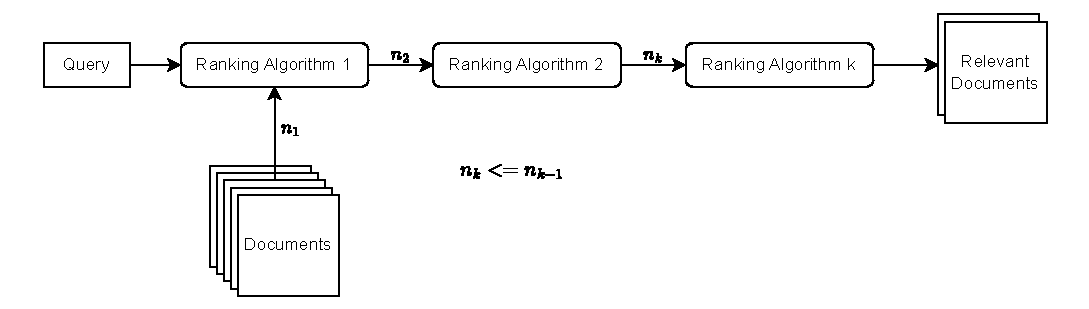
\includegraphics[scale=0.75]{assets/pdfs/CascadeRetrieval.drawio.pdf}
    \caption{Arsitektur \textit{cascaded retrieval}}
    \label{fig:ilustrasi cascade retr}
\end{figure}
Perlu diperhatikan bahwa, untuk setiap tahap \ranking{}, dilakukan penyaringan dan pengurutan dokumen sejumlah \(n_k\) dan dikembalikan dokumen sejumlah \(n_{k+1}\) yang kualitasnya sudah ditingkatkan menggunakan suatu algoritma atau model \ranking{}. Model yang digunakan pada setiap tahap tersebut umumnya dimulai dari suatu algoritma yang efisien seperti algoritma \txt{} \matching{} yang melakukan penyaringan secara \heuristic{}, kemudian diikuti oleh algoritma yang lebih berat secara komputasi seperti model pembelajaran mesin~\citep{zhan2020learning, nguyen2024captain}. Sistem \ir{} dengan arsitektur \cascaded{} inilah yang akan digunakan untuk eksperimen dalam penelitian ini.
%-----------------------------------------------------------------------------%





%-----------------------------------------------------------------------------%
\section{Algoritma \Txt{} \Matching{}}
\label{subbab:2:Algoritma Text Matching}
Algoritma \txt{} \matching{} merupakan algoritma yang umum digunakan sebagai tahap pertama penyaringan dokumen relevan, meskipun kurangnya kemampuan algoritma, seperti \obm{} dan \tfidf{}, dalam menangkap makna semantik dari suatu teks~\citep{zhan2020learning}. Kekurangan algoritma dalam mempertimbangkan makna semantik disebabkan karena perhitungannya yang berfokus pada pencocokan kata. Secara umum, untuk setiap kata \(t\) pada kueri \(q\) dan dokumen \(d\) akan ditentukan bobotnya yang dinotasikan sebagai \(w(t,d)\) dengan \(t\in{}q\). Kemudian, proses \ranking{} menggunakan algoritma tersebut dilakukan dengan mengurutkan skor relevansi \(R\) yang diperoleh menggunakan perhitungan \[
R(q,d)=\sum_{t\in{}q\cap{}d}w(t,d) \, .
\]

\vspace{2mm}
\noindent\textbf{Term Frequency-Inverse Document Frequency (\tfidf{})}. Algoritma ini merupakan salah satu model pembobotan \(w(t,d)\) yang terdiri dari dua bagian. Pertama, bagian \textit{Term Frequency} (TF) sebagai perhitungan frekuensi kemunculan kata pada dokumen yang dinotasikan sebagai
\[
TF(t,d)=\frac{f(t,d)}{len(d)} \, ,
\]
dengan \(f(t,d)\) adalah jumlah kemunculan kata $t$ pada dokumen $d$; dan $len(d)$ ialah jumlah kata pada dokumen $d$. Sementara itu, bagian kedua dari \tfidf{} adalah \textit{Inverse Document Frequency} (IDF) yang memperhitungkan seberapa umum suatu kata dan mengindikasikan seberapa informatif kata tersebut. Bagian ini memberikan bobot yang lebih tinggi untuk kata-kata yang kemunculannya jarang pada kumpulan dokumen dan bobot yang lebih rendah untuk kata-kata yang umum. Bagian IDF dapat dihitung sebagai
\[
IDF(t)= \log\left(\frac{N}{n}\right) \, ,
\]
dengan $N$ sebagai jumlah dokumen pada koleksi; dan $n$ merupakan jumlah dokumen pada koleksi yang mengandung kata $t$. Kedua bagian tersebut digunakan untuk perhitungan bobot \tfidf{} yang dirumuskan dengan
\[ 
w(t,d)=TF(t,d) \times IDF(t) \, . 
\]

\vspace{2mm}
\noindent\textbf{Okapi \obm{}}. Best Matching 25 atau \obm{} merupakan upaya peningkatan efektivitas algoritma \tfidf{}~\citep{schutze2008introduction}. Pendekatan yang diambil oleh~\citet{robertson1995okapi} untuk meningkatkan efektivitas tersebut adalah dengan perhitungan \textit{eliteness}, penambahan normalisasi panjang dokumen, dan saturasi dari TF~\citep{Robertson2009ThePR}. Bobot untuk algoritma \obm{} dapat dihitung sebagai
\[
w(t,d)=\frac{IDF(t) \times TF(t,d) \times (k_1 + 1)}{TF(t,d) + k_1 (1 - b + b \frac{len(d)}{avgdl})} \, ,
\]
% \[
% BM25(q, d) = \sum^M_{i=1} \frac{IDF(t_{i}) \times TF(t_{i},d) \times (k_1 + 1)}{TF(t_{i},d) + k_1 (1 - b + b \frac{len(d)}{avgdl})} \, ,
% \]
dengan $avgdl$ ialah rata-rata panjang dokumen pada korpus; dan nilai parameter bebas $b$ serta $k_1$.

\vspace{2mm}
\noindent\textbf{Divergence from Randomness} (DFR). Dalam penelitian ini akan digunakan juga model yang menggunakan kerangka DFR~\citep{amati2002probabilistic}. Kerangka tersebut merupakan penggabungan dari dua probabilitas yang dirumuskan sebagai $w(t,d)=(1-P_2(t,d))\cdot(-log_2 P_1(t,d))$ dengan $P_1$ merupakan fungsi probabilitas kemunculan kata $t$ di dokumen $d$ sebagai suatu kebetulan dan $P_2$ adalah probabilitas kemunculan suatu kata $t$ yang ditetapkan sebagai kata penting. Terdapat beberapa model yang menerapkan kerangka ini, salah satunya adalah InL2. Model InL2 menerapkan kerangka DFR dengan Laplace's Law of Succession sebagai model probabilitas $P_2$ yang dapat dihitung menggunakan rumus
\[
P(t,d)=\frac{tf}{tf+1} \, ,
\]
dengan $tf$ merupakan nilai $TF(t,d)$ atau kemunculan kata $t$ pada dokumen $d$. Sementara itu, model \textit{Inverse Document Frequency} digunakan sebagai probabilitas $P_1$ yang dirumuskan secara matematis sebagai
\[
P(t,d)=\left(\frac{n+0.5}{N+1}\right)^{tf} \, ,
\]
dengan $n$ yang merupakan jumlah dokumen dari koleksi sejumlah $N$ yang mengandung kata $t$. Selain dari ketiga model yang telah dijelaskan, yaitu \obm{},\tfidf{}, dan InL2, akan dimanfaatkan beberapa model lain yang dapat ditelusuri secara lebih lanjut pada dokumentasi yang telah disediakan pyterrier\footnote{http://terrier.org/docs/current/javadoc/org/terrier/matching/models/package-summary.html}.
%-----------------------------------------------------------------------------%





%-----------------------------------------------------------------------------%
\section{Document Encoder}
\label{subbab:2:Document Encoder}
Untuk memahami makna semantik dari teks kueri dan dokumen, diperlukan model yang mampu mengekstraksi teks dan menghasilkan representasi semantik dalam bentuk vektor. Dalam konteks ini, model transformer akan digunakan untuk mengekstraksi makna semantik dari teks. Model transformer yang diperkenalkan oleh \citet{vaswani2017attention} merupakan salah satu tipe model \nn{} yang telah merevolusi pemrosesan bahasa alami dan bidang kecerdasan buatan lainnya.

Model transformer tersebut terdiri dari lapisan \encoder{} dan \decoder{} yang divisualisasikan pada~\gambar{}~\ref{fig:ilustrasi transformer}.
\begin{figure}[!ht]
    \centering
    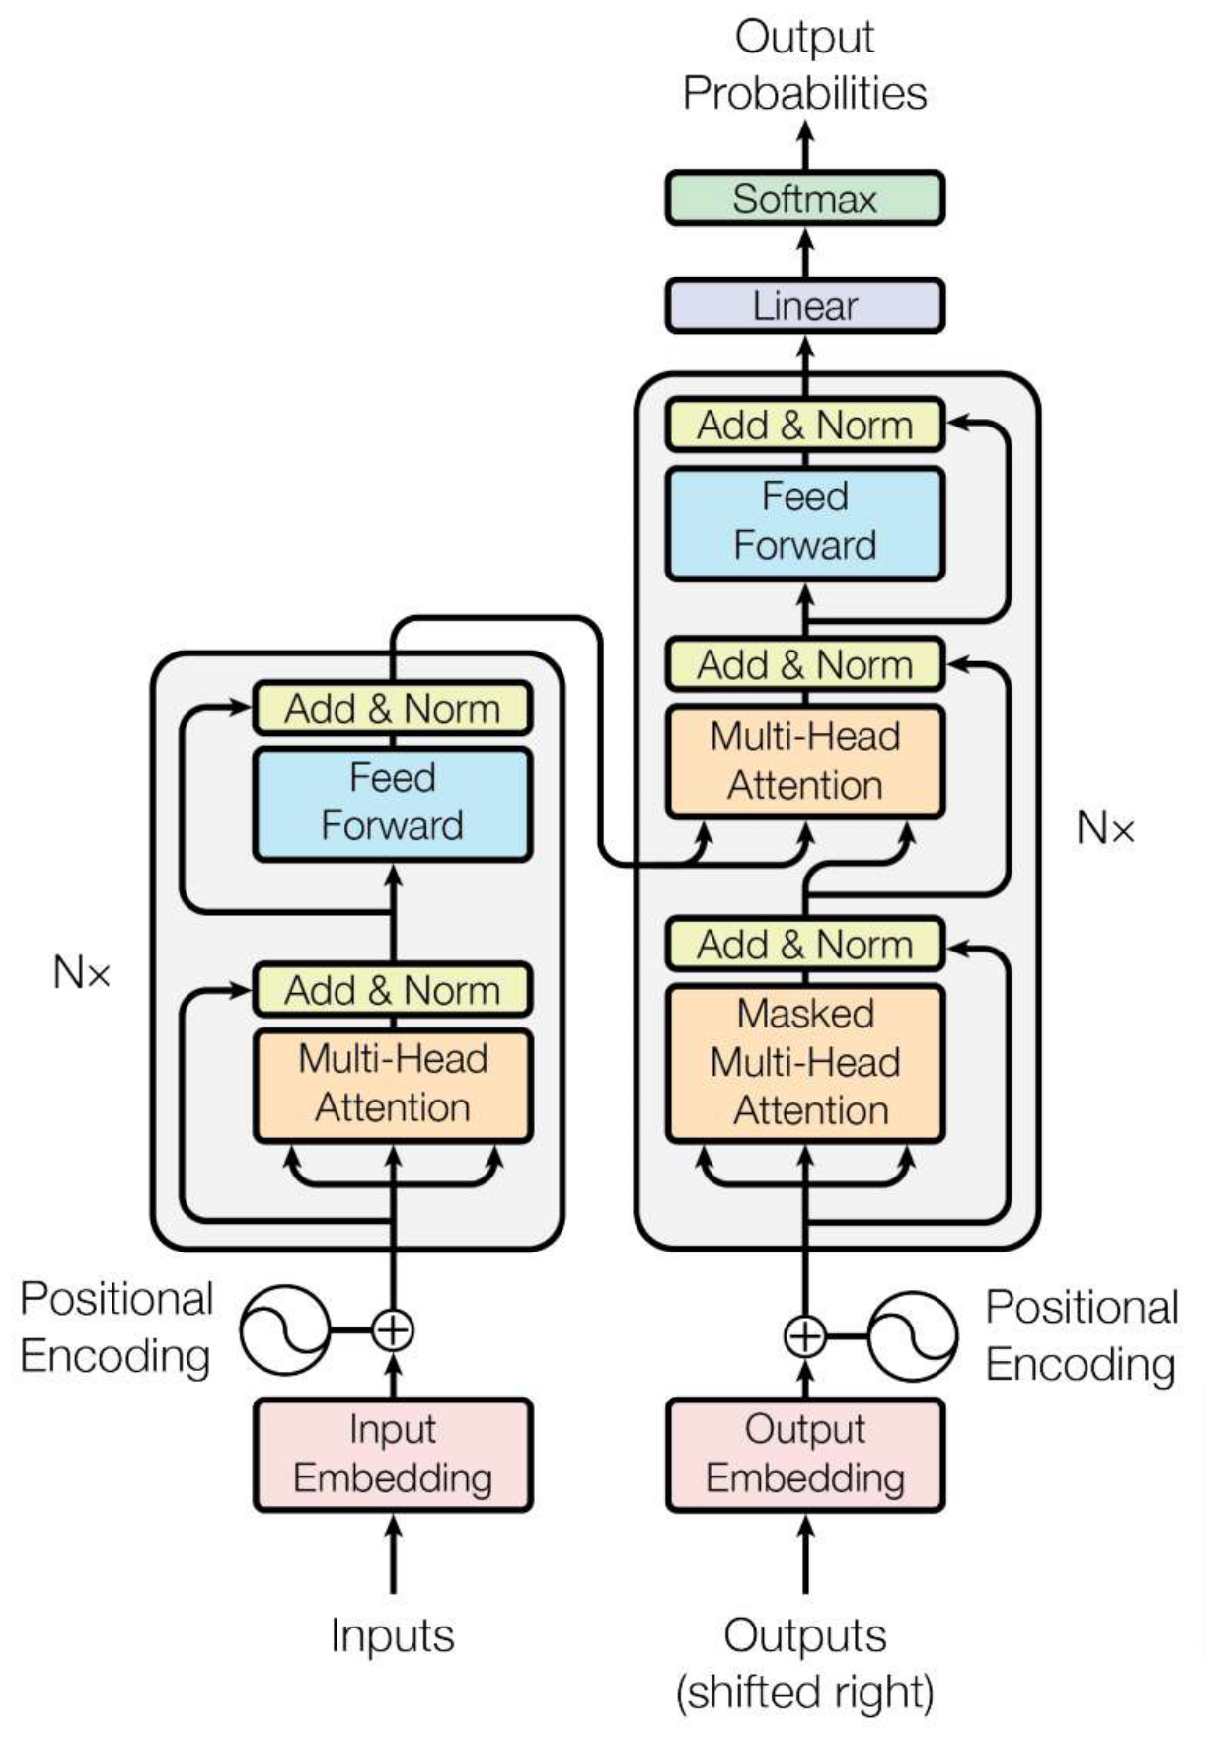
\includegraphics[scale=0.4]{assets/pdfs/transformer_aristektur.pdf}
    \captionsource{Arsitektur transformer}{\citep{vaswani2017attention}}
    \label{fig:ilustrasi transformer}
\end{figure}
Lapisan \encoder{} bekerja dengan mengubah masukan yang berupa teks menjadi vektor yang dapat merepresentasikan makna semantik dari teks tersebut. Kemudian, lapisan \decoder{} digunakan untuk menginterpretasikan vektor hasil lapisan \encoder{} dan menghasilkan serangkaian teks sebagai keluaran. Namun, dalam penelitian ini, karena model transformer hanya diperlukan untuk melakukan ekstraksi hasil vektor representasi teks, maka hanya akan menggunakan lapisan \encoder{} dalam eksperimen.

Pengembangan utama dari arsitektur transformer dibandingkan dengan model-model \nn{} lainnya adalah mekanisme \textit{self-attention} yang memungkinkan model untuk memperhitungkan pentingnya setiap \textit{token} relatif satu sama lain di dalam kalimat. Mekanisme ini memungkinkan model untuk menangkap dependensi atau hubungan tanpa dibatasi oleh jarak antar urutan masukan, suatu hal yang terbatas pada model seperti RNN (Recurrent Neural Network) maupun CNN (Convolutional Neural Network). Namun, karena mekanisme \textit{self-attention} yang tidak mengandalkan alur seperti RNN, maka model transformer perlu mendapatkan informasi tambahan terkait posisi dari \textit{token} dalam urutan. Oleh karena itu, \citet{vaswani2017attention} mengusulkan \textit{positional encoding} agar transformer dapat memanfaatkan informasi dari alur \textit{token}. Selain itu, perlu diperhatikan bahwa untuk setiap \textit{sub-layer} dari \encoder{} dan \decoder{} diimplementasikan \textit{feed-forward network} dan \textit{layer} normalisasi untuk stabilitas dan efisiensi pelatihan.

\vspace{2mm}
\noindent\textbf{\lbert{} (\bert{}).}
\lbert{} (\bert{}) adalah arsitektur yang memanfaatkan bagian \encoder{} dari transformer yang dirancang oleh Google untuk memahami konteks atau makna semantik dari kata di dalam suatu kalimat dengan pendekatan pemrosesan secara \textit{bidirectional}~\citep{devlin2018bert}. Dengan pendekatan ini, \bert{} dapat menangkap hubungan dan konteks antara kata-kata dalam kalimat, baik sebelum atau sesudah kata tertentu. Hal tersebut memungkinkan \bert{} untuk mendapatkan pemahaman yang lebih baik tentang makna kata dalam konteks kalimat yang lebih luas.

Model \bert{} memiliki arsitektur yang memanfaatkan 12 \encoder{} yang bernama \textit{hidden layer} seperti yang ditunjukkan pada \gambar{}~\ref{fig:ilustrasi bert}.
\begin{figure}[!ht]
    \centering
    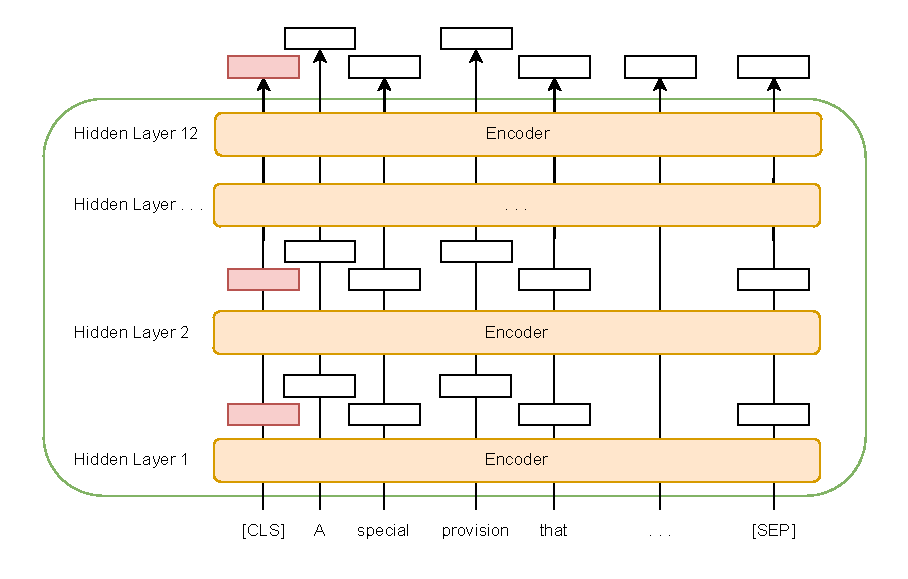
\includegraphics[scale=0.75]{assets/pdfs/IlustrasiBERT.drawio.pdf}
    \caption{Arsitektur model \bert{}}
    \label{fig:ilustrasi bert}
\end{figure}
Perhatikan bahwa masukan untuk model \bert{} merupakan kalimat yang telah dikonversi menjadi \textit{token} dengan tambahan beberapa \textit{token} khusus yang menandakan awal dan akhir kalimat, yaitu ``[CLS]'' dan ``SEP''. Kemudian masukan tersebut akan melewati beberapa pemrosesan oleh \encoder{} sejumlah 12 kali yang dapat dinotasikan sebagai
\[
HS_{n}=ENC_{n}(HS_{n-1}) \, ,
\]
dengan $HS_{n}$ merupakan \hs{} atau keluaran dari \encoder{} pada \textit{layer} ke-$n$; dan $ENC_{n}$ merupakan \encoder{} atau \textit{hidden layer} ke-$n$.

\vspace{2mm}
\noindent\textbf{\ttttt{} (\tfive{}).}
\ttttt{} adalah suatu tipe model yang menerapkan arsitektur transformer. Model ini dirancang untuk berbagai tugas pemrosesan bahasa alami yang secara spesifik dilatih menggunakan kerangka kerja \txt{}-to-\txt{}~\citep{raffel2020exploring}. Berbeda dengan model lain yang dilatih untuk tugas tertentu, model \tfive{} dapat dilatih menggunakan satu tujuan, yaitu mengonversi teks masukan menjadi teks keluaran. Arsitektur \tfive{} serupa dengan \bert{} dengan fokus pada penelitian ini khusus pada bagian \encoder{} dari \tfive{} yang dapat dilihat pada \gambar{}~\ref{fig:ilustrasi t5}
\begin{figure}[!ht]
    \centering
    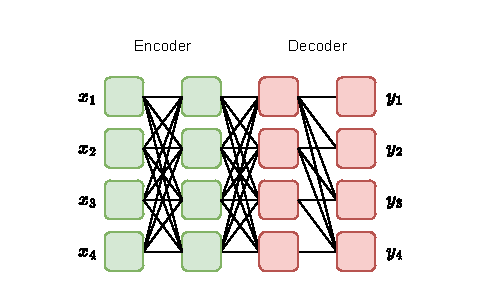
\includegraphics[scale=1.5]{assets/pdfs/t5 structure.drawio.pdf}
    \caption{Arsitektur model \tfive{}}
    \label{fig:ilustrasi t5}
\end{figure}
%-----------------------------------------------------------------------------%





%-----------------------------------------------------------------------------%
\section{Model \Reranker{}}
\label{subbab:2:Model Reranker}
Seperti yang telah dijelaskan pada \bab~\ref{subbab:2:Sistem Information Retrieval}, sebagai suatu upaya perbaikan pada tahap \ranking{} pertama dalam sistem \ir{} dengan arsitektur \cascaded{}, terdapat suatu tahap tambahan, yaitu \reranking{}. Tahap \reranking{} ini, umumnya memerlukan kemampuan komputasi yang lebih tinggi dibanding hanya menggunakan suatu algoritma \txt{} \matching{}~\citep{zhan2020learning}. Salah satu model \reranker{} yang umum digunakan untuk tugas \ranking{} adalah \lambdamart{}, model yang akan digunakan sebagai tahap \ranking{} kedua pada penelitian ini.

\subsection{\ranknet{}}
\label{subbab:2:RankNet}
\ranknet{}~\citep{burges2010ranknet} adalah sebuah model pembelajaran mesin yang dapat  yang secara spesifik dirancang untuk \ltr{} yang digunakan umumnya untuk tugas pemeringkatan seperti \ir{}. Model tersebut dapat diimplementasi menggunakan model \nn{} maupun model \textit{boosted tree} yang menerima suatu vektor $v \in{} \mathbb{R}^n$ dan mengembalikan nilai riil $f(v)$. Diberikan suatu kueri pada pelatihan, \ranknet{} akan terlebih dahulu menghitung skor untuk setiap dokumen dengan $s_{i}=f(v_{i})$, kemudian melakukan komputasi probabilitas $P_{ij}$ yang merupakan kemungkinan dokumen $i$ yang seharusnya ditempatkan pada posisi yang lebih tinggi dibandingkan $j$. Probabilitas tersebut dihitung menggunakan
\[
P_{ij} = \frac{1}{1+e^{-(s_i-s_j)}} \, .
\]

Setelah melakukan komputasi probabilitas untuk setiap pasangan kueri dan dokumen, akan dihitung \textit{cross-entropy loss} $L$ yang didefinisikan sebagai
\[
L=-\bar{P_{ij}}\log{P_{ij}}-(1-\bar{P_{ij}})\log(1-P_{ij}) \, ,
\]
yang kemudian disederhanakan menjadi 
\begin{align*}
L=\frac{(1-S_{ij})}{2}\sigma{}(s_i-s_j)+\log{}(1+e^{-\sigma{}(s_i-s_j)}) \, ,
\end{align*}
dengan $S_{ij}\in{}\{0,\pm{}1\}$ merupakan relevansi yang telah diketahui untuk dokumen yang bernilai 1 ketika dokumen $i$ memiliki label lebih relevan dibanding dokumen $j$, bernilai -1 sebaliknya, dan bernilai 0 ketika label kedua dokumen sama.

\subsection{\lambdarank{}}
\label{subbab:2:LambdaRank}
Model ini merupakan upaya pengembangan \ranknet{} karena saat perancangannya, terdapat asumsi bahwa perhitungan skor masing-masing dokumen merupakan skor yang ideal~\citep{burges2010ranknet}. Salah satu perbedaan \lambdarank{} dan \ranknet{} tidak dibutuhkannya perhitungan \textit{loss} melainkan hanya diperlukan gradien dari nilai tersebut. Gradien tersebut dihitung menggunakan
\[
\lambda_{ij}=\frac{\delta{}L(s_i-s_j)}{\delta{}s_i}=\frac{-\sigma{}}{1+e^{\sigma{}(s_i-s_j)}}|\Delta{}NDCG| \, ,
\]
dengan nilai $NDCG$ sebagai
\begin{align*}
DCG@k&\equiv{}\sum^k_{i=1} \frac{2^{l_i}-1}{\log(1+i)} \, ,\\
NDCG@k&\equiv{}\frac{DCG@k}{maxDCG@k} \, ,
\end{align*}
dengan $k$ merupakan nilai \cutoff{}; dan $l_i$ adalah label dari dokumen $i$. Setelah itu, model melakukan pembaruan bobot menggunakan akumulasi dari gradien tersebut.

\subsection{\lambdamart{}}
\label{subbab:2:LambdaMART}
\lambdamart{} adalah gabungan dari dua buah komponen, yaitu \lambdarank{} dan MART. Multiple Additive Regression Trees (MART) adalah suatu model \textit{ensemble} yang terdiri dari \textit{boosted decision trees}. Dalam model MART, setiap struktur \textit{tree} akan mencoba untuk memperbaiki hasil struktur \textit{tree} sebelumnya untuk meningkatkan kinerja secara menyeluruh. 

Berbeda dengan \lambdarank{} yang memperbarui semua bobot setelah setiap kueri diperiksa. Sebaliknya, dalam \lambdamart{}, keputusan (pemisahan pada \textit{node}) dihitung menggunakan semua data yang berada di \textit{node} tersebut, sehingga \lambdamart{} hanya memperbarui beberapa parameter pada satu waktu. Hal ini berarti LambdaMART dapat memilih pemisahan dan nilai \textit{leaf} yang mungkin menurunkan efektivitas untuk beberapa kueri, asalkan efektivitas keseluruhan meningkat~\citep{burges2010ranknet}.
%-----------------------------------------------------------------------------%

% Dalam penelitian ini, akan dikaji beberapa algoritma yang umum digunakan dalam konteks \ir{} untuk dokumen legal~\citep{goebel2023summary}.
\clearchapter
%-----------------------------------------------------------------------------%
\chapter{\babTiga}
\label{bab:3}
\bab{}~\ref{bab:3} menjelaskan metodologi pada penelitian ini. Pada \subbab{}~\ref{subbab:3:Alur Pekerjaan} dijelaskan langkah-langkah yang dilakukan selama penelitian ini secara keseluruhan.  Kemudian \subbab{}~\ref{subbab:3:Dataset} menerangkan tentang dataset yang digunakan dan pemrosesan yang dilakukan. Setelah itu, \subbab{}~\ref{subbab:3:Pengembangan Sistem Information Retrieval} membahas tentang permasalahan sistem \ir{} dan pendekatan yang diambil oleh peneliti demi meningkatkan efektivitas sistem \ir{} tersebut, yaitu dengan pendekatan model \ml{} berbasis \hcf{} untuk proses \reranking{}.
%-----------------------------------------------------------------------------%





%-----------------------------------------------------------------------------%
\section{Alur Pekerjaan}
\label{subbab:3:Alur Pekerjaan}
Penelitian ini mengkaji fitur yang dapat diekstraksi dari dokumen dan kegunaannya pada proses \reranking{}, khususnya dalam domain legal. Untuk itu, tahap pertama yang dilakukan penulis adalah mengumpulkan data yang sesuai dengan tujuan penelitian, yaitu peraturan beserta beberapa pertanyaan/kasus terkait yang sudah diverifikasi kebenarannya. Setelah mendapatkan data yang sesuai, dilakukan \parsing{} untuk memberikan struktur pada data agar memudahkan pemrosesan data. Kemudian, peneliti mempersiapkan beberapa sistem \ir{} untuk melakukan serangkaian eksperimen.

Eksperimen yang terlebih dahulu dilakukan adalah eksperimen menggunakan beberapa \txt{} \matching{} \alg{} (\base{} \retriever{}) agar dapat ditentukan yang cocok untuk membangun sistem \ir{} dalam domain legal. Sesudah seleksi, peneliti membuat sistem \ir{} menggunakan \base{} \retriever{} yang telah diseleksi untuk analisis melalui beberapa skenario eksperimen.
%-----------------------------------------------------------------------------%
%-----------------------------------------------------------------------------%
\section{Dataset}
\label{subbab:3:Dataset}
Dataset yang dimanfaatkan untuk perancangan sistem \ir{} pada penelitian ini diperoleh dari \coliee{} (\COLIEE{}) 2023, khususnya dataset yang digunakan pada \task{}~3 dan 4~\citep{goebel2023summary}. Dataset tersebut merupakan bagian dari Undang-undang hukum perdata Jepang yang sudah diterjemahkan secara resmi ke dalam bahasa Inggris berupa \txt{} \file{} yang berisi 768 pasal. Pada \gambar{}~\ref{gambar:TextFile}, diberikan pasal pertama yang terletak pada 7 baris paling atas dari \file{} \txt{}.
\begin{figure}[!ht]
    \centering
    \begin{lstlisting}
    Civil Code (Part I, Part II and Part III)
    Part I General Provisions
    Chapter I Common Provisions
    (Fundamental Principles)
    Article 1  (1) Private rights must be congruent with the public welfare.
    (2) The exercise of rights and performance of duties must be done in good faith.
    (3) Abuse of rights is not permitted.\end{lstlisting}
    \caption{Isi dari \file{} civil\_code\_collection.txt}
    \label{gambar:TextFile}
\end{figure}

Selain dari \file{} pasal, terdapat juga \file{} XML yang berisi pasangan kasus (kueri) dan pasal (dokumen) yang relevan. Keseluruhan pasangan yang tersedia diberikan dalam 17 XML \file{} dengan 16 \file{} sebagai data \training{} yang berisi 996 pasang dan 1 \file{} sebagai data \testing{} yang berisi 101 pasang. Contoh isi dari \file{} XML tersebut diberikan pada \gambar{}~\ref{gambar:XMLFile} yang merupakan pasangan pertama dari salah satu \file{} data \training{}.
\begin{figure}[!ht]
    \centering
    \begin{lstlisting}
<?xml version="1.0" encoding="UTF-8" standalone="no"?>
<dataset>
<pair id="H18-1-1" label="Y">
<t1>
Article 572
Even if the seller makes a special agreement to the effect that the seller does not warrant in the case prescribed in the main clause of Article 562, paragraph (1) or Article 565, the seller may not be released from that responsibility with respect to any fact that the seller knew but did not disclose, and with respect to any right that the seller personally created for or assigned to a third party.
</t1>
<t2>
A special provision that releases warranty can be made, but in that situation, when there are rights that the seller establishes on his/her own for a third party, the seller is not released of warranty.
</t2>
</pair>\end{lstlisting}
    \caption{Isi dari \file{} riteval\_H18\_en.xml}
    \label{gambar:XMLFile}
\end{figure}

Struktur dari XML \file{} tersebut berupa sebuah elemen \textit{dataset} yang berisi daftar elemen \textit{pair} dengan atribut \textit{id} dan \textit{label}. Atribut \textit{id} merupakan nilai unik yang diberikan untuk mengidentifikasi setiap kueri, sedangkan \textit{label} melambangkan \textit{entailment} bernilai biner \textit{"Y"}(\textit{entail}) atau \textit{"N"}(\textit{doesn't} \textit{entail}). Namun, karena fokus dari penelitian ini adalah proses \retrieval{} dokumen relevan, maka nilai \textit{entailment} yang merupakan keterhubungan dari kueri dengan dokumen yang relevan tersebut akan diabaikan. Selain atribut yang telah dijelaskan, suatu \textit{pair} juga mengandung 2 elemen, yaitu dokumen-dokumen relevan \(t_1\) dan kueri \(t_2\).

Untuk kedua tipe \file{} tersebut, peneliti melakukan \parsing{} data ke struktur data tabel untuk mempermudah pemrosesan dan analisis yang akan dilakukan terhadap dataset. Terdapat 2 hasil \parsing{} yang dibedakan berdasarkan penanganan karakter spesial, yaitu tanpa penghilangan karakter spesial dan dengan penghilangan karakter spesial. Karakter yang dikategorikan sebagai karakter spesial dalam penelitian ini adalah garis miring '/', kurung buka '(', kurung tutup ')', tanda penghubung '-', dan tanda tanya '?', serta apostrof dan tanda kutip (' dan "). Hasil \parsing{} yang tidak dihilangkan karakter spesialnya digunakan untuk mempertahankan struktur semantik yang diberikan oleh keberadaan karakter tersebut dalam sebuah kalimat. Hal tersebut esensial karena dalam penelitian ini akan digunakan beberapa model \nn{} untuk ekstraksi makna semantik kalimat sebagai salah satu fitur, sehingga diperlukan hasil \parsing{} yang orisinal.

Pada \tabel{}~\ref{tabel:hasil parsing text file} diberikan cuplikan hasil \parsing{} yang dilakukan pada \txt{} \file{}, khususnya hasil dengan penghilangan karakter spesial. Terdapat kolom \txt{} yang memiliki nilai teks dari suatu pasal secara keseluruhan, kolom \textit{docno} sebagai nilai unik setiap pasal yang digunakan untuk identifikasi, dan kolom informasi tambahan mengenai struktur bagian dari pasal tertentu (\textit{part, chap, sect, subsect,} dan \textit{subsubsect}).

\begin{table}[H]
    \centering
    \caption{Hasil \parsing{} pasal (\txt{} \file{})}
    \label{tabel:hasil parsing text file}
    \resizebox{\textwidth}{!}{%
        \begin{tabular}{p{0.425\linewidth}llllll}
        \toprule
        text & docno & part & chap & sect & subsect & subsubsect \\
        \midrule
        Article 1   1  Private rights must be congruent with the public welfare.
         2  The exercise of rights and performance of duties must be done in good faith.
         3  Abuse of rights is not permitted. & 1 & General Provisions & Common Provisions &  &  & Fundamental Principles \\
        Article 2  This Code must be construed so as to honor the dignity of individuals and the essential equality of both sexes. & 2 & General Provisions & Common Provisions &  &  & Standards for Construction \\
        Article 3   1  The enjoyment of private rights commences at birth.
         2  Unless otherwise prohibited by applicable laws, regulations, or treaties, foreign nationals enjoy private rights. & 3 & General Provisions & Persons & Capacity to Hold Rights &  &  \\
        Article 3 2  If the person making a juridical act did not have mental capacity when manifesting the relevant intention, the juridical act is void. & 3-2 & General Provisions & Persons & Mental Capacity &  &  \\
        \bottomrule
        \end{tabular}%
    }
\end{table}

Kemudian, pada \tabel{}~\ref{tabel:hasil parsing xml file}, diberikan cuplikan hasil \parsing{} yang dilakukan pada XML \file{} dengan penghapusan karakter spesial. \tabel{} ini memiliki kolom \textit{qid} yang berisi nilai unik untuk identifikasi kueri, kolom \query{} yang mengandung teks kueri, kolom \entail{} dengan nilai biner \textit{"Y"} atau \textit{"N"} seperti yang dijelaskan sebelumnya, kolom \textit{art} yang berisi teks pasal, dan kolom \textit{art\_code} yang merupakan nilai untuk mengidentifikasi suatu pasal relevan terhadap kueri yang nilainya berhubungan dengan \textit{docno} pada \tabel{}~\ref{tabel:hasil parsing text file}, serta kolom \textit{label} yang bernilai 1 untuk setiap baris sebagai lambang relevansi dari kueri dengan pasal (dokumen) pada baris tersebut.

\begin{table}[H]
    \centering
    \caption{Hasil \parsing{} pasangan kasus-pasal relevan (XML \file{})}
    \label{tabel:hasil parsing xml file}
    \resizebox{\textwidth}{!}{%
        \begin{tabular}{lp{0.275\linewidth}lp{0.375\linewidth}lr}
        \toprule
        qid & query & entail & art & art\_code & label \\
        \midrule
        H18-1-1 & A special provision that releases warranty can be made, but in that situation, when there are rights that the seller establishes on his her own for a third party, the seller is not released of warranty. & Y & Article 572
        Even if the seller makes a special agreement to the effect that the seller does not warrant in the case prescribed in the main clause of Article 562, paragraph  1  or Article 565, the seller may not be released from that responsibility with respect to any fact that the seller knew but did not disclose, and with respect to any right that the seller personally created for or assigned to a third party. & 572 & 1 \\
        H18-1-2 & There is a limitation period on pursuance of warranty if there is restriction due to superficies on the subject matter, but there is no restriction on pursuance of warranty if the seller s rights were revoked due to execution of the mortgage. & N & Article 565
        The provisions of the preceding three Articles apply mutatis mutandis if the right transferred by the seller to the buyer does not conform to the terms of the contract  including the case in which the seller fails to transfer part of a right that belongs to another person . & 565 & 1 \\
        \bottomrule
        \end{tabular}%
    }
\end{table}

Setelah didapatkan data tabel, peneliti melakukan eksplorasi awal data mengenai distribusi jumlah kueri berdasarkan jumlah dokumen relevan yang diidentifikasi untuk setiap kueri. Distribusi tersebut didapatkan oleh peneliti dengan menggunakan data \training{} yang dapat dilihat pada \gambar{}~\ref{gambar:distribusi}.
\begin{figure}[!ht]
    \centering
    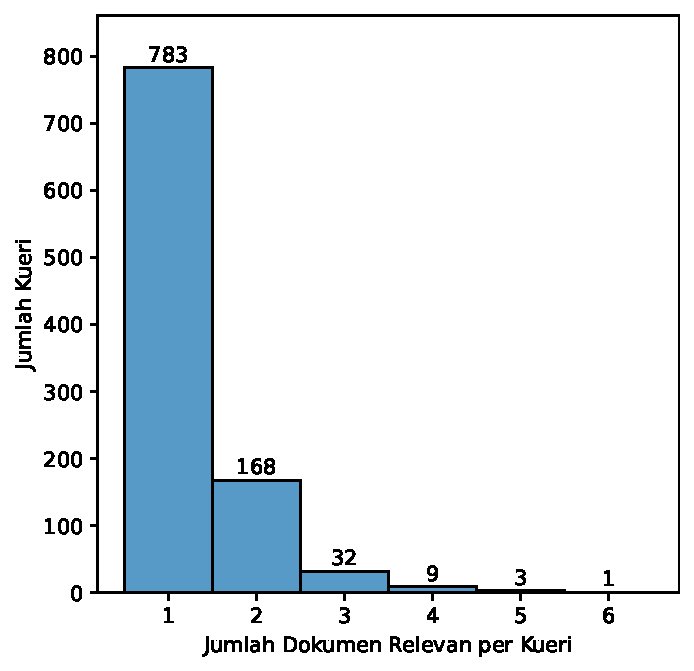
\includegraphics[scale=0.75]{assets/pdfs/Distribusi Query-Dokumen Relevan.pdf}
    \caption{Distribusi jumlah dokumen relevan untuk setiap kueri}
    \label{gambar:distribusi}
\end{figure}
Pada grafik tersebut, dapat dilihat bahwa mayoritas kueri (783) hanya memiliki 1 pasal yang relevan, diikuti oleh 168 kueri yang memiliki 2 pasal relevan dan 32 kueri dengan 3 pasal relevan. Sementara itu, kueri dengan 4 hingga 6 pasal relevan memiliki kontribusi yang kecil terhadap total jumlah kueri, masing-masing tidak lebih dari 10 jumlah kueri dan secara total hanya berkontribusi sekitar 1.31\% untuk data \training{}.
%-----------------------------------------------------------------------------%
%-----------------------------------------------------------------------------%
\section{Pengembangan Sistem \ir{}}
\label{subbab:3:Pengembangan Sistem Information Retrieval}
Peneliti melakukan pengembangan sistem \ir{} dalam bentuk \pipeline{} dengan arsitektur \cascaded{} yang terdiri dari beberapa tahap penyaringan menggunakan algoritma atau fungsi yang semakin kompleks~\citep{wang2011cascade}. \subbab{}~\ref{subbab:3:Pengembangan Sistem Information Retrieval} menjelaskan pengembangan dan pendekatan yang diambil dalam mengembangkan sistem \ir{} untuk domain legal.
%-----------------------------------------------------------------------------%
%-----------------------------------------------------------------------------%
\subsection{Definisi Tugas}
\label{subbab:3:Definisi Tugas}
Fokus dari penelitian ini adalah peningkatan efektivitas proses retrieval menggunakan \hcf{} atau fitur yang dibuat secara manual seperti yang ditunnjukkan pada \gambar{}~\ref{fig:posisiPenelitian}.
\begin{figure}[!ht]
    \centering
    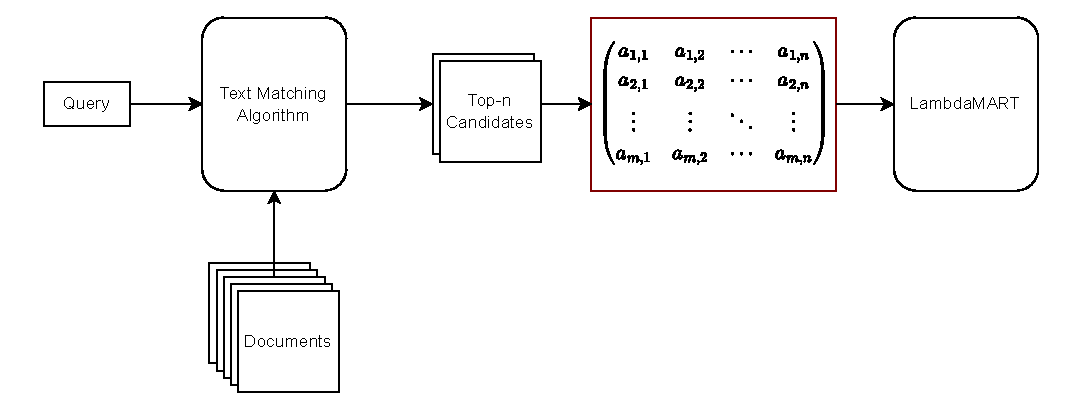
\includegraphics[scale=0.75]{assets/pdfs/PosisiPenelitian.pdf}
    \caption{Bagian dari sistem \ir{} yang akan diteliti}
    \label{fig:posisiPenelitian}
\end{figure}
Proses retrieval dalam konteks ini merujuk pada pengambilan dokumen yang relevan dari sekumpulan dokumen \(D_1,D_2,...,D_k\) berdasarkan kueri \(Q\). Algoritma \txt{} \matching{} digunakan untuk mencocokkan kueri dengan dokumen-dokumen yang ada, menghasilkan urutan dokumen dari yang paling relevan hingga yang paling tidak relevan. Dengan kata lain, algoritma ini memroses kueri dan mengembalikan daftar dokumen \(D_1,D_2,...,D_k\) yang terurut berdasarkan tingkat relevansinya secara menurun. Namun, sistem \ir{} yang hanya mengandalkan pencocokan kata memiliki beberapa kekurangan, seperti tidak diperhitungkannya semantik maupun sinonim dari kata yang dicocokkan~\citep{hambarde2023information}, sehingga sebuah dokumen yang relevan memiliki kemungkinan untuk mendapatkan nilai relevansi yang rendah. Untuk mengatasi kelemahan tersebut, berbagai pendekatan telah dikembangkan demi meningkatkan efektivitas dari sistem \ir{}, seperti pengintegrasian model \ml{}~\citep{burges2010ranknet} atau model \nn{}~\citep{1223700}.

Model \nn{} tidak digunakan dalam penelitian ini karena sifatnya adalah \textit{black box} yang berarti bahwa logika dan cara kerja dari model ini tersembunyi sehingga sulit untuk memahami, melakukan verifikasi, maupun menafsirkan alasan dari keputusan yang dibuat oleh model~\citep{electronics8080832}, terutama dalam bidang \ir{}. Oleh karena itu, peneliti memilih model \ml{}, khususnya \lambdamart{}, dalam pembangunan sistem \ir{} untuk keperluan analisis fitur. Integrasi tersebut akan menerapkan arsitektur \cascaded{}~\citep{wang2011cascade} dengan seleksi 150 dokumen paling relevan oleh algoritma \txt{} \matching{} sebagai tahap pertama mengikuti penelitian terdahulu oleh \citet{nguyen2024captain}. Kemudian, dokumen-dokumen tersebut dipasangkan dengan kueri awal dan dilakukan ekstraksi fitur secara manual yang akan menjadi masukan dari \lambdamart{}. 
%-----------------------------------------------------------------------------%
%-----------------------------------------------------------------------------%
\subsection{Kajian \Base{} \Retriever{}}
\label{subbab:3:Kajian Base Retrieval}
Sebelum melakukan ekstraksi fitur dan meningkatkan efektivitas sistem dengan \lambdamart{} sebagai \reranker{}, peneliti menguji beberapa algoritma \base{} \retriever{} menggunakan data \training{}. \Base{} \retriever{} yang diuji meliputi InL2, DLH13, DFR\_BM25, BM25, DLH, TF\_IDF, LGD, PL2, IFB2, Hiemstra\_LM, DFReeKLIM, DPH, Js\_KLs, DFRee, In\_expB2, In\_expC2, LemurTF\_IDF, DFIZ, InB2, XSqrA\_M, DFIC, BB2, CoordinateMatch, DirichletLM, Tf, dan Dl. Hasil pengujian dapat ditemukan pada \tabel{}~\ref{tabel:3:base retriever}. Berdasarkan hasil tersebut, diseleksi beberapa algoritma untuk skenario penelitian yang akan dilaksanakan selanjutnya.
\begin{table}[!htb]
    \caption{Kinerja \base{} \retriever{} pada data \training{} untuk metrik \recall{}@3}
    \label{tabel:3:base retriever}
    \begin{minipage}{.5\linewidth}
      \centering
        \begin{tabular}{lr}
            \toprule
            name & R@3 \\
            \midrule
            InL2 & 0,6281 \\
            DLH13 & 0,6277 \\
            DFR\_BM25 & 0,6262 \\
            BM25 & 0,6257 \\
            DLH & 0,6247 \\
            TF\_IDF & 0,6214 \\
            LGD & 0,6207 \\
            PL2 & 0,6162 \\
            IFB2 & 0,6159 \\
            Hiemstra\_LM & 0,6154 \\
            DFReeKLIM & 0,6149 \\
            DPH & 0,6146 \\
            Js\_KLs & 0,6146 \\
            \bottomrule
        \end{tabular}
    \end{minipage}
    \begin{minipage}{.5\linewidth}
      \centering
        \begin{tabular}{lr}
            \toprule
            name & R@3 \\
            \midrule
            DFRee & 0,6139 \\
            In\_expB2 & 0,6122 \\
            In\_expC2 & 0,6087 \\
            LemurTF\_IDF & 0,6085 \\
            DFIZ & 0,6082 \\
            InB2 & 0,6060 \\
            XSqrA\_M & 0,6011 \\
            DFIC & 0,5950 \\
            BB2 & 0,5765 \\
            CoordinateMatch & 0,5501 \\
            DirichletLM & 0,5093 \\
            Tf & 0,2562 \\
            Dl & 0,1335 \\
            \bottomrule
        \end{tabular}
    \end{minipage} 
\end{table}

%-----------------------------------------------------------------------------%
%-----------------------------------------------------------------------------%
\subsection{Usulan Fitur}
\label{subbab:3:Usulan Fitur}
Dari setiap pasangan yang dikembalikan \base{} \retriever{}, akan dilakukan ekstraksi berbagai fitur untuk dianalisis penggunaannya dalam proses \reranking{}. Fitur hasil ekstraksi dapat dikategorisasikan ke dalam 3 kelompok, antara lain:

%-----------------------------------------------------------------------------%
\vspace{2mm}
\noindent{}\textbf{Atribut Kuantitatif Sederhana}. Atribut kuantitatif sederhana adalah fitur-fitur dasar yang dapat diekstraksi dari teks tanpa memerlukan perhitungan kompleks atau analisis mendalam. Fitur-fitur ini tidak mempertimbangkan unsur kesamaan antara query dan dokumen, baik secara semantik, struktural, maupun tekstual. Dalam penelitian ini, beberapa fitur kuantitatif sederhana yang dianalisis meliputi jumlah kata pada kueri \(Len(q)\), jumlah kata pada dokumen \(Len(d)\), dan selisih jumlah kata antara kueri-dokumen \(LenDiff\) yang diekspresikan secara matematis sebagai
\[LenDiff(q,d)=|Len(q)-Len(d)| \, ,\]
dengan q sebagai kueri; d merupakan dokumen;dan Len(x) ialah jumlah kata pada x.

%-----------------------------------------------------------------------------%
\vspace{2mm}
\noindent{}\textbf{Skor berbasis \textit{Text Matching}}. Fitur pada kelompok ini berkaitan dengan perhitungan kesamaan antara kueri dan dokumen secara tekstual, seperti yang telah dijelaskan pada \subbab{}~\ref{subbab:2:Algoritma Text Matching}. Beberapa teknik yang akan dianalisis mencakup nilai-nilai relevansi dari \base{} \retriever{} yang dianalisis pada \subbab{}~\ref{subbab:3:Kajian Base Retrieval}. Secara umum, \base{} \retriever{} merupakan suatu algoritma pembobotan atau \weighting{}~\(w(t,d)\) untuk suatu kata atau \term{}~\(t\) pada dokumen~\(d\). Dokumen tersebut biasanya mengandung lebih dari satu \term{}, sehingga, untuk mendapatkan nilai relevansi~\(R\) suatu kueri \(q\) dengan dokumen, diperlukan penggabungan bobot dari setiap \term{}. Salah satu cara yang intuitif adalah dengan menjumlahkan bobot setiap \term{} yang dapat diekspresikan sebagai
\begin{align*}
    R(q,d)=\sum_{t\in{}q\cap{}d}w(t,d) \, .
\end{align*}
    
Nilai relevansi tersebut yang kemudian akan diekstraksi sebagai fitur untuk masukan \reranker{}. Selain nilai relevansi tersebut, dalam penelitian ini akan digunakan juga nilai kesamaan Jaccard \(J(A,B)\) dengan \(A\) dan \(B\) merupakan himpunan \term{} (kata atau frasa) yang didapatkan dari suatu teks. Dalam konteks \ir{}, nilai Jaccard tersebut dapat dikomputasi menggunakan rumus
\begin{align*}
    J(A,B)=\frac{|A\cap{}B|}{|A\cup{}B|};J(A,B)\in{}[0,1] \, ,
\end{align*}
dengan \(A\) merupakan himpunan kata \term{} dari kueri; \(B\) merupakan himpunan \term{} dari dokumen; \(|A\cap{}B|\) adalah jumlah \term{} yang berpotongan antara dokumen dengan kueri; dan \(|A\cup{}B|\) adalah jumlah gabungan \term{} unik dari dokumen dan kueri. Rumus tersebut memiliki nilai dalam interval tertutup 0 hingga 1 secara inklusif, secara spesifik bernilai 0 jika tidak ada \term{} yang sama antara kueri dengan dokumen dan bernilai 1 jika \term{} kueri dan \term{} dokumen identik. Selain menggunakan \term{} yang dibatasi pada kata untuk kesamaan Jaccard, peneliti juga menggunakan frasa dan/atau kata penting yang diekstraksi menggunakan metode yang dikembangkan oleh \citet{rose2010automatic}, yaitu RAKE. \textit{Rapid Automatic Keyword Extraction} (RAKE) adalah metode yang digunakan dalam pemrosesan bahasa alami (NLP) untuk secara otomatis mengidentifikasi kata kunci atau frasa penting pada suatu teks. Peneliti menggunakan RAKE untuk ekstraksi karena tidak diperlukan latihan khusus untuk pemakaiannya serta juga karena sifatnya yang \textit{domain-independent} dan \textit{language-independent}~\citep{rose2010automatic}. Dengan kata lain, penggunaan RAKE tidak terikat pada suatu domain tertentu maupun terbatas pada bahasa yang spesifik.

%-----------------------------------------------------------------------------%
\vspace{2mm}
\noindent{}\textbf{\textit{Semantic Similarity}}. Kelompok ini mengandung fitur-fitur yang berfokus pada kesamaan kontekstual atau semantik antara kueri dan dokumen, bukan hanya kesamaan secara tekstual. Makna atau semantik dari teks tersebut direpresentasikan dengan sebuah vektor yang diperoleh dengan memanfaatkan keluaran model \neural{} \network{}, secara khusus \tfive{} dan \bert{}. Untuk model \bert{}, peneliti menguji beberapa teknik yang diusulkan oleh \citet{devlin2018bert} dengan menggunakan kombinasi dan agregasi dari keluaran \hs{s} \bert{} tanpa \textit{fine-tuning}. Dalam penelitian ini, akan dikaji beberapa usulan \citeauthor{devlin2018bert} dan satu usulan peneliti, yaitu  $LHS\_MEAN$, yang dinotasikan sebagai
% Dengan fungsi $CLS(HS_n)$ merupakan fungsi untuk mengambil vektor \textit{token} pertama hasil keluaran dari suatu \textit{hidden state} $HS_n$, maka dalam penelitian ini, akan digunakan fitur-fitur mengikuti usulan \citeauthor{devlin2018bert} dan satu usulan peneliti ($LHS\_MEAN$)
\begin{align*}
    FHS\_CLS&=CLS(HS_{0}) \, , \\
    STLHS\_CLS&=CLS(HS_{11}) \, , \\
    LHS\_CLS&=CLS(HS_{12}) \, , \\
    SUM\_LFHS\_CLS&=CLS(HS_{9}) + CLS(HS_{10}) + CLS(HS_{11}) + CLS(HS_{12}) \, , \\
    CONCAT\_LFHS\_CLS&=CLS(HS_{9}) \oplus{} CLS(HS_{10}) \oplus{} CLS(HS_{11}) \oplus{} CLS(HS_{12}) \, , \\
    SUM\_AHS\_CLS&=\sum^{12}_{n=1} CLS(HS_{n}) \, , \\
    LHS\_MEAN&=mean(HS_{12}) \, ,
\end{align*}
dengan $HS_{n}$ merupakan vektor keluaran dari $ENC_{n}$ pada \textit{layer} ke-$n$; $CLS(HS_{n})$ adalah fungsi yang mengambil vektor \token{} pertama dari suatu \hs{} $HS_{n}$; dan \textit{mean} ialah fungsi yang menghitung rata-rata pada dimensi kedua, yaitu dimensi \token{}. Perhatikan bahwa simbol $\oplus{}$ merupakan operasi konkatenasi yang menambahkan suatu vektor di akhir vektor lainnya pada suatu dimensi tertentu.

Serupa halnya dengan model \bert{}, peneliti menguji beberapa teknik untuk model \tfive{} yang diusulkan oleh \citet{ni2021sentence}, yaitu dengan menggunakan rata-rata keluaran semua vektor \token{} dari \hs{} terakhir dan vektor \token{} pertama pada \hs{} terakhir yang dinotasikan dengan
\begin{align*}
    LHS\_CLS&=CLS(HS_{12}) \, ,\\
    LHS\_MEAN&=mean(HS_{12}) \, .
\end{align*}

Setelah mendapatkan representasi semantik berupa vektor dari \bert{} dan juga \tfive{}, untuk mengkuantifikasi kemiripan antara kedua representasi tersebut, peneliti menggunakan \textit{cosine similarity} yang umum digunakan dalam penyelesaian tugas pemrosesan bahasa alami~\citep{wehnert2021legal,zhou2022problems}. \textit{Cosine similarity} tersebut dapat diekspresikan dengan persamaan
\begin{align*}
    cosine\_similarity(x_1,x_2)=\frac{x_1\cdot{}x_2}{max(||x_1||_2,\epsilon{})\cdot{}max(||x_2||_2,\epsilon{})} \, ,
\end{align*}
dengan \(x_n\) merupakan vektor; \(\epsilon{}\) adalah konstanta yang sangat kecil (\(\expnumber{1}{-8}\)); dan \(||x_n||_2\) sebagai norma \textit{Euclidean} dari vektor \(x_n\). Konstanta \(\epsilon{}\) tersebut ditambahkan untuk mencegah terjadinya masalah komputasi, yaitu pembagian dengan 0.

%-----------------------------------------------------------------------------%
\subsection{Evaluasi Model}
\label{subbab:3:Evaluasi Model}
Evaluasi yang dilakukan terhadap model dalam penelitian ini mencakup evaluasi hasil menggunakan metrik dan evaluasi korelasi menggunakan koefisien korelasi \textit{pearson}. Metrik, dalam hal ini, akan digunakan untuk membandingkan kinerja antar sistem. Sementara itu, koefisien \textit{pearson} akan dimanfaatkan untuk menentukan hubungan linear dari dua buah variabel yang akan berguna untuk menginvestigasi korelasi antara \cutoff{} dengan efektivitas sistem \ir{}.

\vspace{2mm}
\noindent{}\textbf{Metrik Evaluasi}.
\label{bagian:Metrik Evaluasi}
Model dievaluasi menggunakan metrik yang dihitung berdasarkan urutan dokumen yang dikembalikan. Dari grafik pada \gambar{}~\ref{gambar:distribusi}, didapatkan distribusi yang memiliki rata-rata 1.2771 dan median 1 serta 98.69\% dari kueri tersebut hanya memiliki paling banyak 3 dokumen yang relevan. Karena tujuan dari perancangan sistem \ir{} dalam penelitian ini adalah memperbanyak dokumen relevan yang ditemui pada dokumen teratas untuk keperluan evaluasi oleh badan hukum, maka peneliti menentukan metric \recall{}, secara spesifik pada \cutoff{} 3 atau pada 3 dokumen teratas untuk mengevaluasi kinerja sistem tersebut. Metrik \recall{} dapat dihitung menggunakan rumus
\begin{align*}
    R@k=\frac{TP}{TP+FN} \, ,
\end{align*}
dengan \(R@k\) adalah \recall{} pada \(k\) dokumen teratas; TP merupakan jumlah dokumen diantara $k$ dokumen teratas yang diketahui relevan; dan FN ialah jumlah dokumen relevan yang gagal dikembalikan diantara \(k\) dokumen teratas tersebut. Selain itu, terdapat beberapa metrik yang digunakan untuk keperluan analisis lebih lanjut. Pertama, \textit{precision} yang dapat dihitung sebagai
\[
P@k=\frac{TP}{TP+FP} \, ,
\]
dengan $P@k$ merupakan \textit{precision} pada $k$ dokumen teratas; dan FP ialah jumlah dokumen tidak relevan yang dikembalikan pada $k$ dokumen teratas. Kedua, \textit{reciprocal rank} ($recip\_rank$) yang dinotasikan sebagai
\[
recip\_rank=\frac{1}{rank} \, ,
\]
dengan $rank$ merupakan peringkat dari dokumen relevan teratas. Kemudian, \textit{Mean Average Precision} (MAP) yang dirumuskan sebagai
\begin{align*}
    MAP&=\frac{1}{Q} \sum_{q=1}^Q AP(q) \, ,\\
    AP(q)&=\frac{1}{R} \sum_{n=1}^N P@n \cdot rel@n \, ,
\end{align*}
dengan $Q$ merupakan jumlah kueri yang dievaluasi; $AP(q)$ ialah \textit{average precision} untuk suatu kueri $q$; $R$ adalah jumlah dokumen relevan yang diketahui; $rel@n$ merupakan relevansi dokumen pada posisi $n$; $N$ sebagai jumlah dokumen yang dikembalikan;  Terakhir, terdapat metrik NDCG yang telah didefinisikan pada~\subbab{}~\ref{subbab:2:LambdaRank}

\vspace{2mm}
\noindent{}\textbf{Korelasi \textit{Pearson}}.
\label{bagian:Korelasi Pearson}
Korelasi \textit{pearson} $r$ adalah suatu perhitungan statistik yang mengevaluasi kekuatan dan hubungan linear sepasang variabel. Nilai \textit{pearson} tersebut dapat diperoleh dengan perhitungan
\[
r=\frac{n\sum{}xy-(\sum{}x)(\sum{}y)}{\sqrt{(n\sum{}x^2-(\sum{}x)^2)(n\sum{}y^2-(\sum{}y)^2)}} \, ,
\]
dengan $n$ merupakan jumlah data yang diobservasi; serta $x$ dan $y$ adalah variabel data yang diobservasi.

%-----------------------------------------------------------------------------%
\subsection{Feature Importance}
\label{subbab:3:Feature Importance}
% akan dimanfaatkan sebagai tolok ukur penentuan karakteristik atau fitur yang dapat membantu klasifikasi relevansi antara sepasang kueri dan dokumen.
Evaluasi pemanfaatan fitur merupakan aspek penting dalam mengukur kinerja model, selain dari hasil yang diperoleh melalui metrik. Nilai \textit{feature importance} akan digunakan sebagai tolok ukur penentuan karakteristik atau fitur yang dapat bermanfaat dalam menentukan nilai relevansi antara sepasang kueri dan dokumen. Dalam penelitian ini, nilai \textit{feature importance} dari \lambdamart{} akan digunakan untuk evaluasi pemanfaatan fitur. Model \reranker{} tersebut dipilih karena kemampuannya yang unik dalam mengorbankan kinerja pada kueri tertentu untuk meningkatkan kinerja keseluruhan melalui proses seleksi \textit{split} dan penentuan nilai \textit{leaf}~\citep{burges2010ranknet}. Proses seleksi ini memungkinkan model untuk memilih fitur-fitur yang paling relevan dalam setiap tahap pemisahan data, yang kemudian digunakan untuk mengidentifikasi fitur mana yang paling sering digunakan. Dengan menganalisis frekuensi penggunaan fitur ini, peneliti dapat mengungkap karakteristik penting yang berkontribusi signifikan terhadap tugas penentuan relevansi dokumen legal. Analisis ini memberikan wawasan mendalam mengenai fitur-fitur kunci yang mempengaruhi keputusan model, serta membantu dalam pemahaman yang lebih baik tentang cara kerja model dan langkah-langkah yang dapat diambil untuk meningkatkan kinerjanya lebih lanjut.
% Selain evaluasi hasil menggunakan metrik, peneliti juga melakukan evaluasi pemanfaatan fitur oleh model. Model \reranker{} yang akan digunakan untuk analisis adalah \lambdamart{}, terutama karena kemampuannya dalam memilih untuk mengorbankan kinerja pada kueri tertentu namun meningkatkan kinerja secara keseluruhan dengan melakukan seleksi \textit{split} dan nilai \textit{leaf}~\citep{burges2010ranknet}. Peneliti memanfaatkan hasil seleksi tersebut untuk melakukan analisis frekuensi penggunaan fitur yang menggambarkan karakteristik penting dalam tugas klasifikasi relevansi dokumen legal.
%-----------------------------------------------------------------------------%




% %-----------------------------------------------------------------------------%
% % baseline yang baik untuk \ir{} pada domain legal, yaitu BM25~\citep{DBLP:journals/corr/abs-2105-05686} dan TF-IDF~.
% %-----------------------------------------------------------------------------%



% %-----------------------------------------------------------------------------%
% \section{Analisis Fitur}
% \label{subbab:3:analisisFitur}




% \subsection{Seleksi K-Dokumen Paling Relevan}
% \label{subbab:3:seleksiNDokumenPalingRelevan}

% Proses seleksi k-dokumen paling relevan dilakukan dengan menghitung nilai relevansi setiap pasangan \query{}-dokumen menurut algoritma \base{} \retrieval{}. Setelah mendapat nilai dari setiap pasang, dokumen tersebut akan diurutkan berdasarkan nilai relevansi secara menurun dan diseleksi sejumlah maksimal k-dokumen yang paling relevan. Dokumen yang berhasil dikembalikan oleh proses tersebut kemudian diekstraksi fitur-fiturnya sebagai masukan untuk \reranker{}. Dalam penelitian ini, akan digunakan nilai \cutoff{} \(k=150\) mengikuti \citet{nguyen2024captain} yang berhasil mendapatkan kinerja \(f2\) terbaik pada \COLIEE{} 2023, dengan nilai \(f2\) didapat dari persamaan
% \begin{align*}
% f2=\frac{5 × precision × recall}{4 × precision + recall}
% \end{align*}

% \subsection{Ekstraksi Fitur}
% \label{subbab:3:ekstraksiFitur}

% Dari setiap pasangan yang dikembalikan \base{} \retriever{}, akan dilakukan ekstraksi berbagai fitur untuk dianalisis penggunaannya dalam proses \reranking{}. Fitur hasil ekstraksi dapat dikategorisasikan ke dalam 3 kelompok, antara lain:

% \begin{itemize}[label={}]
%     \item~\textbf{Atribut Kuantitatif Sederhana}. Atribut kuantitatif sederhana adalah fitur-fitur dasar yang dapat diekstraksi dari teks tanpa memerlukan perhitungan yang kompleks atau analisis mendalam. Fitur dalam kelompok ini tidak mempertimbangkan unsur kesamaan antara query dan dokumen, baik secara semantik, struktural, maupun tekstual. Fitur yang akan dianalisis dalam penelitian ini meliputi jumlah kata pada \query{}, jumlah kata pada dokumen, dan Selisih jumlah kata antara \query{}-dokumen.
    
%     \item~\textbf{\Txt{} \Matching{}}. Fitur pada kelompok ini berkaitan dengan perhitungan kesamaan antara \query{} dan dokumen secara tekstual. Beberapa teknik yang akan dianalisis mencakup nilai relevansi dari \base{} \retriever{} yang dianalisis pada \bab~\ref{subbab:3:analisisBaseRetrieval}, nilai Jaccard dari \query{} dan dokumen, serta nilai Jaccard dari hasil ekstraksi RAKE \query{} dan dokumen.
    
%     \item~\textbf{\Semantic{} \Similarity{}}. Fitur yang termasuk dalam kelompok ini berfokus pada kesamaan kontekstual atau semantik antara \query{} dan dokumen, bukan hanya kesamaan secara tekstual. Makna atau semantik dari teks tersebut direpresentasikan dengan sebuah vektor yang diperoleh dengan memanfaatkan beberapa model \neural{} \network{}, yaitu \tfive{} dan \bert{}. Untuk representasi vektor yang digunakan sebagai fitur dari kedua model tersebut, peneliti menguji teknik ekstraksi \citet{devlin2018bert} untuk \bert{} serta beberapa teknik ekstraksi \citet{ni2021sentence} untuk \tfive{}.
% \end{itemize}

% \todo{Ini juga kah pak?
%     \begin{itemize}
%         \item Visualisasi vektor mana yang diambil dari BERT~\citep{devlin2018bert}
%         \item Jelasin visualisasi (\citet{devlin2018bert} ngapain)
%         \item Visualisasi vektor mana yang diambil dari T5~\citep{ni2021sentence}
%         \item Jelasin visualisasi (\citet{ni2021sentence} ngapain)
%     \end{itemize}}



% \subsection{\Reranking{} dengan \lambdamart{}}
% \label{subbab:3:rerankingDenganLambdamart}

% Setelah didapat hasil ekstraksi fitur, sebuah \reranker{} akan digunakan untuk proses \reranking{} dokumen agar dokumen-dokumen yang relevan namun memiliki peringkat yang rendah akan mendapat peringkat yang lebih baik. Dalam penelitian ini, \reranker{} yang akan digunakan adalah \lambdamart{} karena kemampuannya dalam memilih untuk mengorbankan kinerja pada \query{} tertentu namun meningkatkan kinerja secara keseluruhan dengan melakukan seleksi \textit{split} dan nilai \textit{leaf} \citep{burges2010ranknet}.



% \subsection{\Training{} dan Eksperimen}
% \label{subbab:3:rerankerTrainingDanEksperimen}

% Seperti yang telah dijelaskan pada \bab~\ref{subbab:3:analisisFitur}, bahwa akan dirancang sebuah \pipeline{} untuk masing-masing \base{} \retriever{} yang telah ditentukan pada \bab~\ref{subbab:3:analisisBaseRetrieval}, maka akan diperoleh sebanyak 5 \base{} \retriever{} dan 5 sistem \ir{} dengan \reranker{} \lambdamart{}. Model \lambdamart{} akan dilatih menggunakan seluruh fitur pada \bab~\ref{subbab:3:ekstraksiFitur} dan akan dievaluasi kinerjanya dengan membandingkan \base{} \retriever{} yang sesuai. Pelatihan model \lambdamart{} dan evaluasi akan dilakukan dengan teknik \textit{5-fold cross validation} agar diperoleh hasil evaluasi yang dapat mewakilkan kinerja sistem yang sesungguhnya.
% %-----------------------------------------------------------------------------%



% %-----------------------------------------------------------------------------%
% \section{Analisis \Cutoff{} \base{} \retrieval{}}
% \label{subbab:3:analisisCutoffBaseRetrieval}

% Pengujian juga dilakukan pada beberapa \cutoff{} untuk menentukan batasan sedemikian sehingga sistem \ir{} domain legal yang akan dirancang dapat berfungsi dengan efektif dan efisien. Proses pengujian dilakukan seperti yang telah dijelaskan pada \bab~\ref{subbab:3:analisisFitur} dengan perbedaan hanya pada jumlah dokumen yang dikembalikan (\cutoff{}) oleh \base{} \retriever{}. Pada pengujian ini, peneliti memiliki hipotesis bahwa \cutoff{} memiliki korelasi positif dengan kinerja model dengan pengaruh yang semakin kecil dengan bertambahnya \cutoff{} sehingga membentuk suatu kurva asimtot.
% %-----------------------------------------------------------------------------%



% %-----------------------------------------------------------------------------%
% \section{\Incremental{} \Ablation{} \Learning{}}
% \label{subbab:3:ablationLearning}

% Setelah mendapatkan sistem \ir{} dengan \cutoff{} yang paling efektif dari \bab~\ref{subbab:3:analisisCutoffBaseRetrieval}, peneliti akan melakukan analisis pengaruh jumlah fitur terhadap kinerja sistem. Pengujian dilakukan dengan menambahkan jumlah fitur yang digunakan sistem secara inkremental dan melakukan analisis perubahan kinerja sistem. Proses penambahan fitur dilakukan secara terurut dimulai dari fitur dengan \feature{} \importance{} paling tinggi sampai ke yang paling rendah. Dengan melakukan \incremental{} \ablation{} \learning{}, peneliti dapat menentukan jumlah fitur yang efisien untuk perancangan sistem \ir{} domain legal.
% %-----------------------------------------------------------------------------%
\clearchapter
%-----------------------------------------------------------------------------%
\chapter{\babEmpat}
\label{bab:4}
Metodologi yang telah dibahas sebelumnya akan diimplementasikan dengan bantuan program yang akan dibahas pada \bab{}~\ref{bab:4}. Pada \subbab{}~\ref{subbab:4:Persiapan Data}, dijelaskan cara \parsing{} dan pembersihan data yang dilakukan untuk semua \file{} data. Kemudian, \subbab{}~\ref{subbab:4:Implementasi Model} membahas tentang implementasi sistem \ir{} dalam bentuk \pipeline{}. Setelah itu, proses ekstraksi fitur akan disampaikan pada \subbab{}~\ref{subbab:4:Ekstraksi Fitur}. Terakhir, pada \subbab{}~\ref{subbab:4:Evaluasi Model}, akan dijelaskan implementasi kode evaluasi dan perhitungan metrik hasil eksperimen.
%-----------------------------------------------------------------------------%
%-----------------------------------------------------------------------------%
\section{Persiapan Data}
\label{subbab:4:Persiapan Data}
Pada tahap ini, peneliti melakukan persiapan data, meliputi \parsing{} dan pembersihan data. Pertama-tama, \parsing{} dilakukan untuk memberikan struktur pada data sehingga mudah untuk dianalisis maupun diproses lebih lanjut. Setelah itu, data yang telah di-\textit{parse} akan dibersihkan untuk memaksimalkan hasil dari sistem \ir{}. Pada \subbab{}~\ref{subbab:4:Data Pasal}, akan dijelaskan \parsing{} dan pembersihan data pasal (\corpus{}). Kemudian, \subbab{}~\ref{subbab:4:Data Pasangan Kasus-Dokumen Relevan} menyampaikan \parsing{} data kueri-pasal relevan secara lebih rinci.
%-----------------------------------------------------------------------------%
%-----------------------------------------------------------------------------%
\subsection{Data Pasal}
\label{subbab:4:Data Pasal}
Data pasal diberikan dalam bentuk \txt{} \file{} dan belum sepenuhnya terstruktur seperti yang ditunjukkan pada \gambar{}~\ref{gambar:TextFile}. Untuk itu, peneliti mengimplementasi kode untuk melakukan pencocokan struktur dokumen legal pada setiap baris dari \file{} tersebut. Pencocokan struktur ini dilakukan untuk memilah bagian dari dokumen untuk dikonversi ke dalam bentuk tabel. Pada \kode{}~\ref{kode:parsing partition}, dapat dilihat bahwa dilakukan pencocokan baris terhadap struktur dokumen menggunakan \regex{} dengan bantuan \library{} re yang disediakan Python. Pencocokan tersebut dilakukan secara heuristik dengan memanfaatkan kata-kata kunci, seperti \textit{Part}, \textit{Chapter}, \textit{Section}, \textit{Subsection}, dan \textit{Article} yang diikuti penomoran dalam bentuk angka Arab atau Romawi, pada baris 3-13 dan 18-19. Selain itu, terdapat pencocokan struktur bagian yang mengandung satu atau lebih pasal pada baris 15-16. Kemudian, pada baris 21-22, terdapat pencocokan klausa berupa ayat atau kalimat hukum yang merupakan bagian terkecil dari hierarki struktur hukum dan sekaligus merupakan elemen dari suatu pasal atau \textit{article}. Fungsi memilah tersebut kemudian akan digunakan sebagai fungsi pembantu untuk melakukan \parsing{}.
\lstinputlisting[
language=python,
firstline=37,
lastline=58,
label={kode:parsing partition},
caption={Fungsi memilah struktur dokumen legal secara heuristik}
]{assets/codes/data_parsing.py}

Proses \parsing{} yang diimplementasikan pada \kode{}~\ref{kode:parsing pasal} merupakan algoritma sederhana yang mengiterasi setiap baris dalam \file{} kemudian melakukan salah satu dari dua hal, yaitu melakukan pencatatan pasal atau menyesuaikan struktur hierarki dari baris yang diiterasi. Pencatatan pasal diimplementasikan pada baris 9-11 yang melakukan penambahan klausa hukum untuk suatu pasal yang sedang diiterasi, serta pada baris 13-14 dan 35-36 yang melakukan finalisasi iterasi pasal dengan menambahkannya ke dalam \textit{list}. Selain itu, penyesuaian struktur hierarki hukum dapat diliihat pada baris 16-30 yang melakukan perubahan sesuai dengan struktur yang ditemui saat iterasi. Perubahan yang dimaksud terjadi ketika baris yang diiterasi beranjak dari suatu hierarki aturan ke hierarki lain yang sebanding atau lebih tinggi, sehingga data hierarki yang lebih rendah akan dihapus karena sudah tidak relevan dengan pasal pada bagian selanjutnya. Perhatikan bahwa walaupun masih dalam satu rantai pernyataan \lstinline{if-else}, baris 31-33 melakukan hal yang berbeda, yaitu mencatat baris yang menandakan awal mula iterasi pasal dan menyimpan kode unik yang dimiliki oleh setiap pasal.
\lstinputlisting[
language=python,
firstline=64,
lastline=101,
label={kode:parsing pasal},
caption={Fungsi \parsing{} pasal sebagai \corpus{}}
]{assets/codes/data_parsing.py}

Setelah itu, diimplementasikan fungsi penanganan karakter spesial pada \kode{}~\ref{kode:penanganan karakter spesial} untuk menghindari terjadinya \error{} pada saat proses \retrieval{} yang disebabkan oleh keberadaan karakter spesial.
\lstinputlisting[
language=python,
firstline=107,
lastline=109,
label={kode:penanganan karakter spesial},
caption={Penanganan karakter spesial}
]{assets/codes/data_parsing.py}

Kemudian, \kode{}~\ref{kode:tabelisasi} mengonversi list yang didapat dari \kode{}~\ref{kode:parsing pasal} ke dalam bentuk tabel yang dapat dilihat pada baris 4-8. Perlu diperhatikan bahwa, pada baris 4, \parsing{} dilakukan dengan melewatkan baris pertama yang hanya berisi judul dari dokumen hukum. Kemudian, penghilangan karakter spesial dapat dilihat pada baris 10-11 dengan fungsi pembantu \kode{}~\ref{kode:penanganan karakter spesial}. Namun, seperti yang dijelaskan pada \subbab{}~\ref{subbab:3:Dataset} bahwa hilangnya keberadaan karakter-karakter spesial dapat menyebabkan makna semantik suatu kalimat untuk berubah karena bergantinya struktur kalimat tersebut. Oleh karena itu, diimplementasikan juga versi tanpa penghapusan karakter spesial yang dapat dilihat pada baris 16-18. Sehabis itu, kolom data tabel diatur ulang agar kolom yang esensial termasuk dalam kolom-kolom pertama sebelum dikembalikan.
\lstinputlisting[
language=python,
firstline=113,
lastline=132,
label={kode:tabelisasi},
caption={Konversi \corpus{} menjadi bentuk tabel}
]{assets/codes/data_parsing.py}

Sehabis implementasi fungsi \parsing{}, \kode{}~\ref{kode:tabelisasi} dijalankan dengan memasukkan lokasi \txt{} \file{} sebagai argumen dan hasilnya disimpan dalam variabel yang dapat ditemui pada \kode{}~\ref{kode:gunsi}. Terdapat 2 versi tabel yang disimpan, yaitu \lstinline{articles} sebagai tabel yang mengandung teks tanpa karakter spesial dan \lstinline{encoder_articles} yang masih mengandung karakter spesial pada teks.
\lstinputlisting[
language=python,
firstline=138,
lastline=139,
label={kode:gunsi},
caption={Melakukan \parsing{} \txt{} \file{} dan menyimpan hasil}
]{assets/codes/data_parsing.py}

Setelah menyimpan kedua tabel ke dalam variabel, dilakukan eksplorasi sederhana terhadap teks hasil \parsing{} untuk menginvestigasi kemungkinan kesalahan dari implementasi \parsing{} yang telah dibuat. Berdasarkan eksplorasi tersebut, ditemukan bahwa ada beberapa duplikasi data sehingga dilakukan penghapusan data duplikat yang implementasinya dapat dilihat pada \kode{}~\ref{kode:pemusnahan duplikasi}.
\lstinputlisting[
language=python,
firstline=147,
lastline=148,
label={kode:pemusnahan duplikasi},
caption={Penanganan duplikasi data}
]{assets/codes/data_parsing.py}
Selain duplikasi data, ditemukan juga beberapa pasal valid namun tidak informatif yang tidak tereliminasi dengan \parsing{} secara heuristik yang telah diimplementasikan. Pasal tidak informatif tersebut merupakan pasal yang dihapus dari dokumen hukum seperti yang ditunjukkan pada \tabel{}~\ref{tabel:deleted article}.
\begin{table}[H]
    \centering
    \caption{Data hasil \parsing{} yang tidak berlaku dan sudah dihapus}
    \label{tabel:deleted article}
    \resizebox{\textwidth}{!}{%
        \begin{tabular}{lllp{0.125\linewidth}lp{0.225\linewidth}p{0.4\linewidth}}
        \toprule
        text & docno & part & chap & sect & subsect & subsubsect \\
        \midrule
        Article 208  Deleted & 208 & Real Rights & Ownership & Extent of Ownership & Content and Scope of Ownership & Scope of Ownership in Land \\
        Article 363  Deleted & 363 & Real Rights & Pledges & Pledges of Rights &  & Subject Matter of Pledges of Rights \\
        Article 365  Deleted & 365 & Real Rights & Pledges & Pledges of Rights &  & Requirements for Perfection of Pledges over Claims \\
        Article 367  Deleted & 367 & Real Rights & Pledges & Pledges of Rights &  & Collection of Claims by Pledgees \\
        Article 368  Deleted & 368 & Real Rights & Pledges & Pledges of Rights &  & Collection of Claims by Pledgees \\
        Article 480  Deleted & 480 & Claims & General Provisions & Extinction of Claims & Performance & Performance to Holder of Receipt \\
        Article 571  Deleted & 571 & Claims & Contracts & Sale & Effect of Sale & Buyer's Demand for Reimbursement of Expenses for Immovables Subject to Mortgage \\
        Article 635  Deleted & 635 & Claims & Contracts & Contracts for Work &  & Remuneration in Proportion to Benefit Received by Party Ordering Work \\
        \bottomrule
        \end{tabular}%
    }
\end{table}
Oleh karena itu, dilakukan pembersihan data dengan menggunakan pencocokan kata sederhana yang implementasinya terdapat pada \kode{}~\ref{kode:pemusnahan deleted}.
\lstinputlisting[
language=python,
firstline=184,
lastline=188,
label={kode:pemusnahan deleted},
caption={Pembersihan data}
]{assets/codes/data_parsing.py}
%-----------------------------------------------------------------------------%
%-----------------------------------------------------------------------------%
\subsection{Data Pasangan Kasus-Dokumen Relevan}
\label{subbab:4:Data Pasangan Kasus-Dokumen Relevan}
Pada tahapan selanjutnya, \parsing{} yang berbeda  dengan \subbab{}~\ref{subbab:4:Data Pasal} diimplementasikan untuk data pasangan kueri-pasal relevan yang telah diberikan pada \gambar{}~\ref{tabel:hasil parsing xml file}. Agar memudahkan proses \parsing{} suatu data XML, maka akan dimanfaatkan \library{} xml yang disediakan oleh Python yang memungkinkan akses elemen XML secara langsung. Pertama, diimplementasikan suatu fungsi pembantu untuk mengambil teks dari suatu elemen XML. Implementasi dari fungsi tersebut dapat ditemukan di \kode{}~\ref{kode:penculikan anak pertama}.
\lstinputlisting[
language=python,
firstline=204,
lastline=207,
label={kode:penculikan anak pertama},
caption={Fungsi pembantu untuk ekstraksi elemen XML}
]{assets/codes/data_parsing.py}

Kemudian, peneliti membuat implementasi \parsing{} untuk seluruh XML \file{} yang dapat dilihat pada \kode{}~\ref{kode:tabelisasi xml}. Perhatikan bahwa digunakan \library{} glob dari Python untuk memperoleh suatu daftar lokasi \file{} XML pada baris 6.
\lstinputlisting[
language=python,
firstline=209,
lastline=244,
label={kode:tabelisasi xml},
caption={Fungsi \parsing{} dan konversi ke dalam bentuk tabel}
]{assets/codes/data_parsing.py}
Dibandingkan dengan \parsing{} pada \subbab{}~\ref{subbab:4:Data Pasal}, \parsing{} untuk data XML lebih sederhana karena strukturnya yang sudah jelas. Dapat dilihat bahwa, fungsi tersebut diimplementasikan dengan mengiterasi setiap elemen \textit{pair} kemudian memasangkan kueri pada elemen \textit{t2} dengan setiap pasal relevan yang dapat ditemukan pada elemen \textit{t1}. Diimplementasikan juga untuk fungsi tanpa penghilangan karakter spesial pada baris ke-34.

Fungsi tersebut kemudian dijalankan dengan argumen lokasi \textit{directory} yang berisi data \training{} dan \testing{} sesuai dengan pembagian dataset kompetisi \COLIEE{} 2023, untuk versi tanpa penghapusan karakter spesial, serta dengan penghapusan karakter spesial yang dapat dilihat pada \kode{}~\ref{kode:xunsi}. 
\lstinputlisting[
language=python,
firstline=250,
lastline=255,
label={kode:xunsi},
caption={Melakukan \parsing{} XML dan menyimpan hasil}
]{assets/codes/data_parsing.py}
%-----------------------------------------------------------------------------%
%-----------------------------------------------------------------------------%
\section{Implementasi Model}
\label{subbab:4:Implementasi Model}
Setelah data sudah siap dipakai, dipersiapkan implementasi program untuk membangun sistem \ir{} dalam bentuk \pipeline{}. \Pipeline{} yang dimaksud adalah suatu elemen pemrosesan data yang diatur secara berurutan dengan keluaran dari satu elemen akan menjadi masukan ke elemen berikutnya sampai diperoleh hasil akhir yang diinginkan. Dalam konteks \cascaded{} \ir{} yang ingin dirancang pada penelitian ini, akan dibentuk 3 buah \pipeline{}, yaitu \pipeline{} tahap \ranking{} pertama, \pipeline{} ekstraksi fitur, dan \pipeline{} tahap \ranking{} kedua menggunakan \lambdamart{}. Dalam penelitian ini, digunakan \library{} pyterrier dalam perancangan ketiga \pipeline{} tersebut. Agar dapat memanfaatkan pyterrier, perlu dieksekusi \kode{}~\ref{kode:init terrier} yang menjalankan program Terrier.jar sudah ada atau mengunduhnya terlebih dahulu sebelum dijalankan.
\begin{lstlisting}[language=Python, caption={Menjalankan program Terrier}, label={kode:init terrier}]
pt.init(version='5.x-SNAPSHOT', helper_version='0.0.8')
\end{lstlisting}

Sebelum melakukan proses \retrieval{}, agar dapat berjalan dengan efisien, dilakukan pembuatan indeks dokumen terlebih dahulu. Implementasi pembuatan indeks dapat dilihat pada \kode{}~\ref{kode:indexing}. Perhatikan bahwa, pada baris 1, dibentuk suatu objek yang dapat membuat indeks dalam bentuk \textit{blocks} dengan menerima parameter lokasi pembuatan indeks. Kemudian, pada baris 2, dibuat indeks untuk tabel pasal hasil \parsing{} \subbab{}~\ref{subbab:4:Persiapan Data}. Untuk membuat indeks tersebut, diberikan 2 argumen, pertama sebagai basis pembuatan \textit{inverted index} dan yang kedua adalah metadata yang ingin disimpan pada indeks.
\begin{lstlisting}[language=Python, caption={Pembentukan indeks}, label={kode:indexing}]
import pyterrier as pt

pd_indexer = pt.DFIndexer(os.path.join(DIR, 'coliee_index'), blocks=True)
index_ref = pd_indexer.index(articles["text"], articles)
\end{lstlisting}

Sehabis membentuk indeks, dilakukan perancangan \pipeline{} untuk analisis efektivitas berbagai \base{} \retriever{}. Pembentukan \pipeline{} tersebut diimplementasikan pada \kode{}~\ref{kode:init_retr}. Perhatikan bahwa pada baris 1-4 didaftarkan beberapa nama model atau algoritma \base{} \retrieval{}, kemudian untuk setiap model tersebut dibangun \pipeline{} \retrieval{} sebagai tahap \ranking{} pertama pada baris 6-8.
\begin{lstlisting}[language=Python, caption={Pembentukan \textit{Base retriever pipelines}}, label={kode:init_retr}]
models = ['BB2', 'BM25', 'CoordinateMatch', 'DFIC', 'DFIZ', 'DFR_BM25', 'DFRee',
          'DFReeKLIM', 'DirichletLM', 'Dl', 'DLH', 'DLH13', 'DPH', 'XSqrA_M',
          'Hiemstra_LM', 'IFB2', 'In_expB2', 'In_expC2', 'InB2', 'InL2',
          'Js_KLs', 'LemurTF_IDF', 'LGD', 'PL2', 'Tf', 'TF_IDF']

init_retrs = {model_name: pt.BatchRetrieve(index_ref, wmodel=model_name)
              for model_name
              in models}
\end{lstlisting}

Model yang terdaftar dalam bentuk \textit{dictionary} kemudian dipisahkan \textit{key} dan \textit{value}-nya menjadi 2 \textit{list}, yang berisi nama model dan \pipeline{}, untuk keperluan eksperimen\retrieval{}. Implementasi pemisahan tersebut dapat ditemukan di \kode{}~\ref{kode:init_retr_for_exp} yang melakukan iterasi terhadap setiap elemen pada \textit{dictionary}.
\begin{lstlisting}[language=Python, caption={Persiapan \textit{base retriever pipelines} untuk Eksperimen}, label={kode:init_retr_for_exp}]
model_names = []
base_pipelines = []

for name, init_retr in init_retrs.items():
    model_names.append(name)
    base_pipelines.append(init_retr)
\end{lstlisting}

Kedua \textit{list} yang didapat dari \kode{}~\ref{kode:init_retr_for_exp} digunakan sebagai argumen untuk eksperimen dengan memanfaatkan fungsi pyterrier.Experiment yang implementasinya dapat dilihat pada \kode{}~\ref{kode:init_retr_exp}. Pada baris 7, diberikan argumen indeks dari \obm{} pada \textit{list} yang akan digunakan sebagai \baseline{} pada eksperimen ini. Selain itu, terdapat beberapa argumen lain pada baris 3-5, yang akan didefinisikan pada \subbab{}~\ref{subbab:4:Evaluasi Model}.
\begin{lstlisting}[language=Python, caption={Eksperimen berbagai model atau algoritma \base{} \retrieval{}}, label={kode:init_retr_exp}]
experiment_data = pt.Experiment(
    retr_systems=base_pipelines,
    topics=dev_topics,
    qrels=qrels,
    eval_metrics=metrics,
    names=model_names,
    baseline=model_names.index('BM25'))
\end{lstlisting}

Setelah melakukan seleksi model yang akan digunakan untuk analisis pada eksperimen-eksperimen berikutnya, akan dibangun \pipeline{} untuk \ranking{} pertama model-model tersebut. Implementasi pembentukan \pipeline{} dapat dilihat pada \kode{}~\ref{kode:pipe first}, serupa dengan pembentukan sebelumnya, dengan tambahan notasi \lstinline{% cut_off} untuk membatasi jumlah dokumen yang dikembalikan dalam tahap \ranking{} pertama pada sistem \cascaded{} \ir{}. Seperti yang telah dijelaskan pada \subbab{}~\ref{subbab:3:Definisi Tugas}, nilai dari cut\_off dalam sistem yang akan dibuat adalah 150.
\begin{lstlisting}[language=Python, caption={\Pipeline{} tahap \ranking{} pertama}, label={kode:pipe first}]
bm25 = pt.BatchRetrieve(index_ref, wmodel='BM25') % cut_off
tfidf = pt.BatchRetrieve(index_ref, wmodel='TF_IDF') % cut_off
dlh13 = pt.BatchRetrieve(index_ref, wmodel='DLH13') % cut_off
inl2 = pt.BatchRetrieve(index_ref, wmodel='InL2') % cut_off
dfr_bm25 = pt.BatchRetrieve(index_ref, wmodel='DFR_BM25') % cut_off
\end{lstlisting}

Kemudian, untuk setiap sistem, akan ditambahkan \pipeline{} yang mengambil teks dokumen dari indeks untuk keperluan ekstraksi fitur. Hal tersebut dilakukan karena teks tidak secara otomatis dikembalikan bersama proses \retrieval{} pada \ranking{} tahap pertama. Pada \kode{}~\ref{kode:pipe get text}, terdapat implementasi pembuatan \pipeline{} pengambilan teks dengan fungsi pyterrier.text.get\_text dan penyambungan kedua \pipeline{} dengan notasi \lstinline{>>}.
\begin{lstlisting}[language=Python, caption={Pengambilan teks dokumen pada \pipeline{}}, label={kode:pipe get text}]
pipe_bm25 = bm25 >> pt.text.get_text(index_ref, "text")
pipe_tfidf = tfidf >> pt.text.get_text(index_ref, "text")
pipe_dlh13 = dlh13 >> pt.text.get_text(index_ref, "text")
pipe_inl2 = inl2 >> pt.text.get_text(index_ref, "text")
pipe_dfr_bm25 = dfr_bm25 >> pt.text.get_text(index_ref, "text")
\end{lstlisting}

Sehabis itu, dengan cara yang sama, \pipeline{} gabungan yang didapat pada \kode{}~\ref{kode:pipe get text} akan disambung dengan \pipeline{} berikutnya, yaitu \pipeline{} ekstraksi fitur. Implementasi tersebut dapat ditemukan pada \kode{}~\ref{kode:pipe get feature}. \Pipeline{} all\_features bertugas melakukan komputasi nilai-nilai fitur yang menjadi usulan yang telah dibahas pada \subbab{}~\ref{subbab:3:Usulan Fitur} untuk setiap pasangan kueri-dokumen hasil keluaran dari \pipeline{} sebelumnya dan implementasinya baru akan dijelaskan pada \subbab{}~\ref{subbab:4:Ekstraksi Fitur}.
\begin{lstlisting}[language=Python, caption={\Pipeline{} ekstraksi fitur}, label={kode:pipe get feature}]
pipe_bm25_all = pipe_bm25 >> all_features
pipe_dlh13_all = pipe_dlh13 >> all_features
pipe_inl2_all = pipe_inl2 >> all_features
pipe_tfidf_all = pipe_tfidf >> all_features
pipe_dfr_bm25_all = pipe_dfr_bm25 >> all_features
\end{lstlisting}

Sebelum membangun \pipeline{} tahap \ranking{} terakhir, dipersiapkan terlebih dahulu fungsi untuk membangun model \lambdamart{} yang diimplementasikan pada \kode{}~\ref{kode:fun mart}. Dimanfaatkan \textit{library} xgb yang disediakan oleh XGBoost untuk mengonstruksi \lambdamart{} dengan menyesuaikan parameter optimasi, yaitu objective, sebagai NDCG. Terdapat beberapa juga penyesuaian parameter lain, mengikuti saran \textit{library} pyterrier yang secara umum dilakukan untuk mencegah overfitting, seperti learning\_rate dan min\_child\_weight yang lebih kecil, serta gamma yang lebih besar.
\begin{lstlisting}[language=Python, caption={Pembentukan model \lambdamart{}}, label={kode:fun mart}]
import xgboost as xgb

def get_new_lambdamart():
    return xgb.sklearn.XGBRanker(
        objective='rank:ndcg',
        learning_rate=0.1,
        gamma=1.0,
        min_child_weight=0.1,
        random_state=42)
\end{lstlisting}

Kemudian, pada \kode{}~\ref{kode:pipe rerank init} dilakukan pencocokan antar nama \pipeline{}, \pipeline{}, dan \reranker{} \lambdamart{} yang diperoleh pada \kode{}~\ref{kode:fun mart}. Penamaan yang digunakan untuk sistem \ir{} dengan \reranker{} mengikuti format \lstinline{<base_retriever> (Re-ranker)}. Perhatikan bahwa \lambdamart{} hanya dikonstruksi sekali untuk melakukan eksperimen karena setiap pelatihan yang dilakukan akan mengubah seluruh bobot pada model \lambdamart{}, dalam arti lain, pelatihan yang dilakukan akan independen terhadap hasil pelatihan-pelatihan sebelumnya.
\begin{lstlisting}[language=Python, caption={Pencocokan \pipeline{} \reranker{}}, label={kode:pipe rerank init}]
rerankers_pipe = {'BM25 (Re-ranker)': pipe_bm25_all,
                  'DLH13 (Re-ranker)': pipe_dlh13_all,
                  'InL2 (Re-ranker)': pipe_inl2_all,
                  'TF_IDF (Re-ranker)': pipe_tfidf_all,
                  'DFR_BM25 (Re-ranker)': pipe_dfr_bm25_all}

rerankers = {'BM25 (Re-ranker)': get_new_lambdamart(),
             'DLH13 (Re-ranker)': get_new_lambdamart(),
             'InL2 (Re-ranker)': get_new_lambdamart(),
             'TF_IDF (Re-ranker)': get_new_lambdamart(),
             'DFR_BM25 (Re-ranker)': get_new_lambdamart()}
\end{lstlisting}

Setelah dicocokkan nama dengan \pipeline{} yang sesuai, akan dilakukan penyambungan \pipeline{} ekstraksi fitur yang diperoleh pada \kode{}~\ref{kode:pipe get feature} dengan \pipeline{} tahap \ranking{} kedua, yaitu \pipeline{} \reranker{}. Konstruksi \pipeline{} \reranker{} memanfaatkan fungsi pyterrier.ltr.apply\_learned\_model yang mengintegrasi \lambdamart{} sebagai \pipeline{}. \kode{}~\ref{kode:pipe rerank append} mengimplementasi keseluruhan proses pembuatan \pipeline{} \reranker{} dan penyambungannya ke \pipeline{} sebelumnya.
\begin{lstlisting}[language=Python, caption={Pembuatan dan penyambungan \pipeline{} \reranker{}}, label={kode:pipe rerank append}]
pipelines_with_reranker = {
    reranker_name: rerankers_pipe[reranker_name] >> pt.ltr.apply_learned_model(
        rerankers[reranker_name], form="ltr")
    for reranker_name in rerankers
}\end{lstlisting}

Sampai tahap ini, sistem \ir{} yang akan dianalisis sudah berhasil dikonstruksi. Oleh karena itu, berikutnya akan dilakukan persiapan untuk eksperimen. Pertama, dilakukan pendaftaran \base{} \retriever{} yang akan digunakan untuk pembanding saat eksperimen beserta pendekatan yang diusulkan dalam rupa sistem \ir{} yang implementasinya dapat ditemukan pada \kode{}~\ref{kode:daftar tanding}. Perlu diperhatikan bahwa, pada baris 13-14 dan 20-22, dilakukan pemisahan untuk sistem yang dilengkapi dengan \reranker{}. Hal tersebut dilakukan karena, dalam penelitian ini, dimanfaatkan suatu model \ml{}, sehingga terdapat kebutuhan pelatihan sebelum sistem dapat digunakan untuk menjalankan eksperimen.
\begin{lstlisting}[language=Python, caption={Pendaftaran model untuk eksperimen}, label={kode:daftar tanding}]
matching_alg = {
    'BM25': bm25,
    'TF_IDF': tfidf,
    'DLH13': dlh13,
    'InL2': inl2,
    'DFR_BM25': dfr_bm25
}

pipeline_agg = matching_alg | pipelines_with_reranker

pipeline_names = []
pipelines = []
pipeline_names_with_fit = []
pipelines_with_fit = []

for pipe_name, feature in pipeline_agg.items():
    pipeline_names.append(pipe_name)
    pipelines.append(feature)

    if pipe_name in pipelines_with_reranker:
        pipeline_names_with_fit.append(pipe_name)
        pipelines_with_fit.append(feature)
\end{lstlisting}

Pelatihan dilakukan untuk sistem yang memiliki \pipeline{} \reranker{} seperti yang telah dijelaskan sebelumnya. Untuk melatih \lambdamart{}, digunakan sebagian dari data \training{}, terlepas dari data yang digunakan untuk eksperimen maupun data \testing{}. \kode{}~\ref{kode:training reranker} mengandung implementasi program yang digunakan untuk melatih \reranker{} pada sistem \ir{} tersebut. Dapat dilihat bahwa, untuk setiap \pipeline{}, pelatihan menggunakan fungsi fit dengan argumen \_train\_topics dan \_val\_topics yang merupakan himpunan kueri yang berasal dari data \training{}, serta qrels yang merupakan himpunan pasangan kueri-dokumen relevan.
\begin{lstlisting}[language=Python, caption={Pelatihan model \reranker{}}, label={kode:training reranker}]
for i, pipeline in enumerate(pipelines_with_fit):
    pipeline.fit(_train_topics, qrels, _val_topics, qrels)
\end{lstlisting}

Sesudah melatih seluruh \reranker{}, dilakukan eksperimen yang menggunakan data \_val\_topics untuk evaluasi kinerja setiap sistem. Serupa dengan eksperimen sebelumnya, akan dimanfaatkan fungsi pr.Experiment untuk penilaian kinerja sistem yang dapat dilihat implementasinya pada \kode{}~\ref{kode:experiment reranker}. Terdapat sedikit perbedaan argumen eksperimen, yaitu perquery, untuk melakukan evaluasi kinerja pada tiap kueri.
\begin{lstlisting}[language=Python, caption={Eksperimen \retrieval{}}, label={kode:experiment reranker}]
experiment_data = pt.Experiment(
    retr_systems=pipelines,
    topics=_val_topics,
    qrels=qrels,
    eval_metrics=metrics,
    names=pipeline_names,
    perquery=True,
    verbose=True)
\end{lstlisting}

Metrik yang dihasilkan untuk setiap kueri tersebut kemudian diagregasi dengan bantuan fungsi \kode{}~\ref{kode:agg metric}. Perhatikan bahwa agregasi kinerja dilakukan dengan rata-rata.
\begin{lstlisting}[language=Python, caption={Agregasi metrik hasil eksperimen}, label={kode:agg metric}]
def agg_metrics(
    data: pd.DataFrame,
    drop_col: list[str] = ['qid'],
    group_col: Optional[str] = None,
) -> pd.DataFrame:
    _group_col = ['name']
    if group_col:
        _group_col.append(group_col)

    return data.drop(columns=drop_col).groupby(_group_col, as_index=False).mean()
\end{lstlisting}
%-----------------------------------------------------------------------------%
%-----------------------------------------------------------------------------%
\section{Ekstraksi Fitur}
\label{subbab:4:Ekstraksi Fitur}
Seperti yang telah disinggung di \subbab{}~\ref{subbab:4:Implementasi Model} bahwa terdapat \pipeline{} khusus yang akan digunakan untuk melakukan ekstraksi fitur, yaitu \pipeline{} all\_features pada \kode{}~\ref{kode:pipe get feature}. \subbab{}~\ref{subbab:4:Ekstraksi Fitur} membahas tentang implementasi proses ekstraksi fitur-fitur yang telah diusulkan pada \subbab{}~\ref{subbab:3:Usulan Fitur}. Secara garis besar, fitur yang akan diekstraksi dapat dibagi ke dalam 3 kelompok yang akan dijelaskan implementasinya pada \subbab{}~\ref{subbab:4:Ekstraksi Fitur:Atribut Kuantitatif Sederhana} untuk atribut kuantitatif sederhana, \subbab{}~\ref{subbab:4:Ekstraksi Fitur:Text Matching Score} untuk fitur skor \txt{} \matching{}, dan \subbab{}~\ref{subbab:4:Ekstraksi Fitur:Semantic Similarity} untuk pemanfaatan hasil \encoder{} sebagai fitur. Fitur-fitur tersebut akan diekstraksi dari hasil keluaran \pipeline{} sebelumnya, \kode{}~\ref{kode:pipe get text}, yang dapat dilihat cuplikannya pada \tabel{}~\ref{tabel:keluaran pertama} yang mengandung hasil kembalian paling relevan dari pipe\_bm25.
\begin{table}[H]
    \centering
    \caption{Cuplikan keluaran \pipeline{} tahap \ranking{} pertama}
    \label{tabel:keluaran pertama}
    \resizebox{\textwidth}{!}{%
        \begin{tabular}{lrlrrp{0.225\linewidth}p{0.375\linewidth}}
        \toprule
        qid & docid & docno & rank & score & query & text \\
        \midrule
        H21-26-U & 654 & 620 & 0 & 18.152 & The cancellation of a partnership contract  shall solely become effective toward the future. & Article 620  If a lease is cancelled, the cancellation becomes effective solely toward the future. In such a case, the cancellation does not preclude a claim for compensation for loss or damage. \\
        \bottomrule
        \end{tabular}
    }
\end{table}

\subsection{Atribut Kuantitatif Sederhana}
\label{subbab:4:Ekstraksi Fitur:Atribut Kuantitatif Sederhana}
% \vspace{2mm}
% \noindent{}\textbf{Atribut Kuantitatif Sederhana}.

Berdasarkan yang telah dibahas pada \subbab{}~\ref{subbab:3:Usulan Fitur}, fitur usulan yang termasuk dalam kelompok ini hanya memanfaatkan atribut kuantitatif yang bisa didapatkan dari suatu teks, tanpa memperhitungkan kesamaan tekstual maupun semantik antara teks kueri dan teks dokumen. Terdapat 3 fitur usulan yang termasuk ke dalam kelompok ini, antara lain jumlah kata pada teks kueri, jumlah kata pada teks dokumen, dan selisih jumlah kata antara teks kueri dan teks dokumen. Pertama, diimplementasikan suatu fungsi untuk menghitung jumlah kata pada teks yang dapat dilihat pada \kode{}~\ref{kode:fungsi fitur jumlah kata}. Perhatikan bahwa nilai yang akan dimanfaatkan sebagai fitur, pada baris 7 dan 16, dikembalikan dalam bentuk numpy.ndarray. Pembungkusan hasil perhitungan tersebut ke dalam numpy.ndarray dilakukan agar dapat memanfaatkan fungsi penggabungan fitur yang disediakan pyterrier.


\begin{lstlisting}[language=Python, caption={Fungsi fitur jumlah kata}, label={kode:fungsi fitur jumlah kata}]
import numpy as np

def f_word_length(string: str) -> int:
    return len(string.split())

def word_length(string: str) -> np.ndarray[int]:
    return np.array([f_word_length(string)])

def f_word_length_diff(query: str, document: str) -> int:
    query_length = f_word_length(query)
    document_length = f_word_length(document)
    return abs(query_length - document_length)

def word_length_diff(query: str, document: str) -> np.ndarray[int]:
    diff = f_word_length_diff(query, document)
    return np.array([diff])
\end{lstlisting}

Fungsi yang telah didefinisikan pada \kode{}~\ref{kode:fungsi fitur jumlah kata} akan digunakan untuk mengekstraksi fitur dari pasangan kueri-dokumen yang dikembalikan oleh tahap \ranking{} pertama yang contohnya dapat dilihat pada \tabel{}~\ref{tabel:keluaran pertama}. \Pipeline{} ekstraksi dibuat dengan fungsi pyterrier.apply.doc\_features menggunakan fungsi \lstinline{lambda} yang dapat ditemukan pada \kode{}~\ref{kode:fitur jumlah kata}. Pada baris 1-9, didapatkan fitur jumlah kata pada kueri maupun dokumen. Sementara itu, pada baris 11-14 diperoleh selisih antara jumlah kata yang terdapat pada kueri dan dokumen sebagai fitur.
\begin{lstlisting}[language=Python, caption={\Pipeline{} ekstraksi fitur jumlah kata}, label={kode:fitur jumlah kata}]
query_length = pt.apply.doc_features(
    lambda query_doc:
    word_length(query_doc['query'])
)

document_length = pt.apply.doc_features(
    lambda query_doc:
    word_length(query_doc['text'])
)

query_document_length_diff = pt.apply.doc_features(
    lambda query_doc:
    word_length_diff(query_doc['query'], query_doc['text'])
)
\end{lstlisting}








\subsection{Skor Berbasis \textit{Text Matching}}
\label{subbab:4:Ekstraksi Fitur:Text Matching Score}
% \vspace{2mm}
% \noindent{}\textbf{Text Matching Score}

Pada kelompok ini, akan dimanfaatkan model-model \base{} \retriever{} untuk melakukan perhitungan skor seperti kolom score yang dapat ditemukan pada \tabel{}~\ref{tabel:keluaran pertama}. Skor yang didapat dari perhitungan model tersebut kemudian akan digunakan sebagai salah satu fitur. Pada \kode{}~\ref{kode:pembentukan model untuk ekstraksi fitur} akan dibentuk \pipeline{} untuk setiap model \base{} \retriever{} yang akan digunakan sebagai fitur. Perlu diperhatikan bahwa dilakukan penghapusan 5 model \base{} \retriever{} yang terpilih untuk sistem \ir{}, namun hal tersebut hanya dilakukan agar tidak terjadi ekstraksi lebih dari satu kali untuk model yang sama.
\begin{lstlisting}[language=Python, caption={\Pipeline{} ekstraksi fitur skor \base{} \retriever{}}, label={kode:pembentukan model untuk ekstraksi fitur}]
base_models = ['BM25', 'TF_IDF', 'DLH13', 'InL2', 'DFR_BM25']
other_models = ['BB2', 'BM25', 'CoordinateMatch', 'DFIC', 'DFIZ', 'DFR_BM25', 'DFRee',
                'DFReeKLIM', 'DirichletLM', 'Dl', 'DLH', 'DLH13', 'DPH', 'XSqrA_M',
                'Hiemstra_LM', 'IFB2', 'In_expB2', 'In_expC2', 'InB2', 'InL2',
                'Js_KLs', 'LemurTF_IDF', 'LGD', 'PL2', 'Tf', 'TF_IDF']

for _model in base_models:
    other_models.remove(_model) 

other_matching_alg = [pt.BatchRetrieve(index_ref, wmodel=model_name) % cut_off
                      for model_name in other_models]
\end{lstlisting}

Selain perhitungan dari model-model berbasis \txt{} \matching{} tersebut, dalam kelompok ini juga terdapat fitur usulan jaccard dan rake\_jaccard seperti yang telah dijelaskan pada \subbab{}~\ref{subbab:3:Usulan Fitur}. Sebelum membentuk \pipeline{} untuk kedua fitur tersebut, diimplementasikan algoritma RAKE terlebih dahulu. Perlu diperhatikan bahwa untuk mengimplementasi alforitma RAKE, akan digunakan beberapa \library{}, yaitu nltk dan rake\_nltk. Kemudian, karena algoritma ingin diimplementasi juga untuk bahasa Indonesia, maka diperlukan beberapa data yang perlu diunduh terlebih dahulu. \kode{}~\ref{kode:dependency rake} melakukan pengunduhan data \textit{stopwords} dan \textit{punkt} sebagai dependensi dari \library{} rake\_nltk, serta pengunduhan \textit{stopwords} untuk bahasa Indonesia\footnote{https://github.com/stopwords-iso/stopwords-id.git}.
\begin{lstlisting}[language=Python, caption={Dependensi algoritma RAKE}, label={kode:dependency rake}]
import json
import nltk

from rake_nltk import Rake
from nltk.tokenize import RegexpTokenizer

assert nltk.download('stopwords')
assert nltk.download('punkt')

with open(IDN_STOPWORDS_DIR) as f:
  idn_stopwords = json.load(f)
\end{lstlisting}

Setelah dependensi berhasil diunduh, RAKE diimplementasi dengan bantuan \textit{library} rake\_nltk yang dapat ditemukan pada \kode{}~\ref{kode:rake}. Ekstraksi dilakukan dengan menginisialisasi rake\_nltk.Rake menggunakan daftar stopwords, sesuai bahasa yang diinginkan, sebagai argumen. Kemudian, kata kunci atau frasa penting dalam suatu teks dapat diekstraksi dengan memanggil fungsi seperti pada baris 10.
\begin{lstlisting}[language=Python, caption={Implementasi RAKE}, label={kode:rake}]
def extract_keywords_rake(
    text: str,
    language: Optional[str]=None,
    with_scores: bool=False
):
    if language is None or language == 'english':
        r = Rake()
    elif language == 'indonesian':
        r = Rake(stopwords=idn_stopwords)
    r.extract_keywords_from_text(text)
    
    return r.get_ranked_phrases()
\end{lstlisting}

Kesamaan jaccard diimplementasikan pada \kode{}~\ref{kode:fungsi fitur jaccard}, secara spesifik pada dua baris pertama. Fungsi tersebut menerima dua buah himpunan kata kemudian dilakukan pembagian jumlah irisan kata dari himpunan-himpunan tersebut oleh jumlah kata unik dari kedua himpunan. Kemudian, fungsi tersebut dimanfaatkan dengan beberapa kombinasi metode, antara lain dengan RAKE pada baris 14-19 atau \regex{} pada baris 22-24. 
Untuk metode \regex{}, kesamaan jaccard dihitung berdasarkan himpunan kata yang ditemukan dalam teks. Sementara itu, metode RAKE menghitung kesamaan jaccard berdasarkan himpunan frasa atau kata penting yang berhasil diekstraksi dari teks.
\begin{lstlisting}[language=Python, caption={Fungsi fitur jaccard}, label={kode:fungsi fitur jaccard}]
def f_jaccard(query_set, document_set):
  return len(query_set & document_set) / len(query_set | document_set)

VALID_LANGUAGE = [None, 'english', 'indonesian']
def jaccard(
    query: str,
    document: str,
    rake: bool=False,
    language: Optional[str]=None
):
  query = query.lower()
  document = document.lower()

  if rake:
    if language not in VALID_LANGUAGE:
        raise ValueError("language must be one of %r" % VALID_LANGUAGE)

    query_set = set(extract_keywords_rake(query, language=language))
    document_set = set(extract_keywords_rake(document, language=language))

  else:
    tokenizer = RegexpTokenizer(r'[\w]+')
    query_set = set(tokenizer.tokenize(query))
    document_set = set(tokenizer.tokenize(document))

  return np.array([
      f_jaccard(query_set, document_set)
  ])
\end{lstlisting}


Setelah diimplementasikan fungsi kesamaan jaccard, dibentuk dua buah \pipeline{}, versi dengan RAKE dan tanpa RAKE, yang dapat ditemukan pada \kode{}~\ref{kode:fitur jaccard}. Pada implementasi tersebut, versi \pipeline{} dengan \regex{} dapat ditemukan di baris 1-4, sedangkan versi \pipeline{} dengan RAKE dapat dilihat pada baris 6-9.
\begin{lstlisting}[language=Python, caption={\Pipeline{} ekstraksi fitur jaccard}, label={kode:fitur jaccard}]
jaccard_score = pt.apply.doc_features(
    lambda query_doc:
    jaccard(query_doc['query'], query_doc['text'], rake=False)
)

rake_jaccard_score = pt.apply.doc_features(
    lambda query_doc: jaccard(
        query_doc['query'], query_doc['text'], rake=True)
)
\end{lstlisting}


\subsection{Semantic Similarity}
\label{subbab:4:Ekstraksi Fitur:Semantic Similarity}
% \vspace{2mm}
% \noindent{}\textbf{Semantic Similarity}
Untuk mendapatkan makna semantik dari suatu teks, digunakan \encoder{} dari \llm{} (\LLM{}). Model tersebut menerima sebuah teks dan mengeluarkan vektor representasi dari teks tersebut yang dapat dikaitkan dengan makna semantik dari teks atau yang biasa dikenal sebagai vektor \embedding{}. Terdapat beberapa model LLM yang diusulkan untuk dimanfaatkan \encoder{}-nya, seperti \bert{}\footnote{https://huggingface.co/google-bert/bert-base-uncased} dan \tfive{}\footnote{https://huggingface.co/BeIR/query-gen-msmarco-t5-base-v1}. Kedua model \LLM{} tersebut diunduh dan dimuat konfigurasinya oleh \kode{}~\ref{kode:load llms}.
\begin{lstlisting}[language=Python, caption={\textit{Load} \encoder{} dan model yang sudah dilatih}, label={kode:load llms}]
from transformers import BertTokenizer, BertModel, \
    T5Tokenizer, T5EncoderModel, PreTrainedTokenizer, PreTrainedModel

bert_tokenizer = BertTokenizer.from_pretrained('google-bert/bert-base-uncased')
bert_model = BertModel.from_pretrained('google-bert/bert-base-uncased')

t5_tokenizer = T5Tokenizer.from_pretrained('BeIR/query-gen-msmarco-t5-base-v1')
t5_model = T5EncoderModel.from_pretrained('BeIR/query-gen-msmarco-t5-base-v1')
\end{lstlisting}


Setelah memuat model beserta \textit{tokenizer} untuk \bert{} dan \tfive{}, diimplementasikan fungsi pada \kode{}~\ref{kode:input encoder} untuk memperoleh vektor dari semua \hs{} yang kombinasinya akan diuji pada eksperimen selanjutnya. Perhatikan bahwa teks perlu di-\textit{tokenize} terlebih dahulu untuk mendapatkan representasinya dalam bentuk angka sebelum dapat dimasukkan ke \encoder{}. Proses \textit{tokenize} tersebut diimplementasikan pada baris ke-6 dengan argumen tambahan \lstinline{truncation} yang akan memotong jumlah \textit{token} yang dikembalikan jika sudah melebihi batas. Kemudian daftar \textit{token} yang dikembalikan akan menjadi masukan dari \encoder{}, begitu juga untuk argumen \lstinline{output_hidden_states} yang diatur untuk bernilai \lstinline{True} agar \encoder{} mengembalikan seluruh keluaran \hs{}.

\begin{lstlisting}[language=Python, caption={Fungsi mendapatkan keluaran dari \encoder{}}, label={kode:input encoder}]
def get_model_outputs(
    string: str,
    tokenizer: PreTrainedTokenizer,
    model: PreTrainedModel
):
    encoded_string = tokenizer(string, return_tensors='pt', truncation=True)
    model_output = model(**encoded_string, output_hidden_states=True)
    return model_output
\end{lstlisting}


Pada \kode{}~\ref{kode:get hss} berikut, diimplementasikan pengambilan keluaran beberapa \hs{s} dari \encoder{} yang dipakai. Bisa dilihat bahwa \lstinline{last_hidden_state_feature_vector} merupakan fungsi yang mengembalikan nilai keluaran dari \hs{} terakhir, sedangkan \lstinline{all_hidden_state_feature_vector}  mengembalikan nilai keluaran dari seluruh \hs{s}.
\begin{lstlisting}[language=Python, caption={Fungsi pengambilan \hs{}}, label={kode:get hss}]
def last_hidden_state_feature_vector(
    string: str,
    tokenizer: PreTrainedTokenizer,
    model: PreTrainedModel
):
    model_output = get_model_outputs(
        string=string, tokenizer=tokenizer, model=model)
    return model_output.last_hidden_state

def all_hidden_state_feature_vector(
    string: str,
    tokenizer: PreTrainedTokenizer,
    model: PreTrainedModel
):
    model_output = get_model_outputs(
        string=string, tokenizer=tokenizer, model=model)
    return model_output.hidden_states
\end{lstlisting}


Setelah diimplementasikan fungsi yang mengambil beberapa keluaran \hs{s}, pada \kode{}~\ref{kode:get cls}, diberikan implementasi pengambilan vektor pertama dari suatu \hs{}. Perhatikan bahwa digunakan \library{} torch untuk mengonversi keluaran model yang berupa \lstinline{tuple} menjadi bentuk \lstinline{torch.tensor}. Sehabis itu, dilakukan pengambilan vektor \textit{token} pertama dari setiap \hs{s} dengan pemotongan \lstinline{[:, 0, :]}. Perhatikan bahwa terdapat 3 dimensi dari hasil kembalian \lstinline{all_hidden_state_feature_vector} yang secara terurut mewakilkan \hs{}, \textit{token}, dan vektor.
\begin{lstlisting}[language=Python, caption={Pengambilan vektor pertama keluaran \hs{}}, label={kode:get cls}]
import torch

def get_cls(
    string: str,
    tokenizer: PreTrainedTokenizer,
    model: PreTrainedModel,
):
    model_output = all_hidden_state_feature_vector(
        string=string,
        tokenizer=tokenizer,
        model=model
    )
    hidden_states_tensor = torch.cat(model_output)
    return hidden_states_tensor[:, 0, :]
\end{lstlisting}





Kemudian, diimplementasikan beberapa metode pemanfaatan vektor dari keluaran \hs{s} yang akan dijadikan sebagai representasi teks, seperti yang telah dijelaskan pada \subbab{}~\ref{subbab:3:Usulan Fitur}. Implementasi pemanfaatan vektor tersebut dapat dilihat di \kode{}~\ref{kode:get which hs}. Perlu diperhatikan bahwa dilewatkan \hs{} pertama pada \lstinline{sum_ahs_cls} karena, untuk \bert{}, keluaran \hs{} yang dikembalikan sejumlah 13 dengan \hs{} pertama yang lebih dikenal sebagai \embedding{}.
\begin{lstlisting}[language=Python, caption={Metode pengambilan vektor dari \hs{}}, label={kode:get which hs}]
def lhs_mean(
    string: str,
    tokenizer: PreTrainedTokenizer,
    model: PreTrainedModel
):
    model_output = last_hidden_state_feature_vector(
        string=string,
        tokenizer=tokenizer,
        model=model
    )
    return model_output.mean(dim=1).flatten().detach()

def fhs_cls(
    string: str,
    tokenizer: PreTrainedTokenizer,
    model: PreTrainedModel,
):
    hidden_states_cls = get_cls(string=string, tokenizer=tokenizer, model=model)
    return hidden_states_cls[0].detach()

def lhs_cls(
    string: str,
    tokenizer: PreTrainedTokenizer,
    model: PreTrainedModel,
):
    hidden_states_cls = get_cls(string=string, tokenizer=tokenizer, model=model)
    return hidden_states_cls[-1].detach()

def stlhs_cls(
    string: str,
    tokenizer: PreTrainedTokenizer,
    model: PreTrainedModel,
):
    hidden_states_cls = get_cls(string=string, tokenizer=tokenizer, model=model)
    return hidden_states_cls[-2].detach()

def sum_ahs_cls(
    string: str,
    tokenizer: PreTrainedTokenizer,
    model: PreTrainedModel,
):
    hidden_states_cls = get_cls(string=string, tokenizer=tokenizer, model=model)
    return hidden_states_cls[1:].sum(dim=0).detach()

def sum_lfhs_cls(
    string: str,
    tokenizer: PreTrainedTokenizer,
    model: PreTrainedModel,
):
    hidden_states_cls = get_cls(string=string, tokenizer=tokenizer, model=model)
    return hidden_states_cls[-4:].sum(dim=0).detach()

def concat_lfhs_cls(
    string: str,
    tokenizer: PreTrainedTokenizer,
    model: PreTrainedModel,
):
    hidden_states_cls = get_cls(string=string, tokenizer=tokenizer, model=model)
    return hidden_states_cls[-4:].flatten().detach()
\end{lstlisting}








Sehabis mendefinisikan beberapa metode pengambilan vektor keluaran \hs{}, fungsi tersebut dibungkus dalam fungsi \lstinline{lambda} yang dapat ditemukan pada \kode{}~\ref{kode:fungsi lambda encoder} untuk beberapa usulan fitur yang akan diuji. Terdapat 7 metode pengambilan yang akan diuji untuk penggunaan \bert{}, diantaranya \lstinline{get_bert_lhs_mean} yang merupakan usulan dari peneliti, kemudian 6 sisanya merupakan usulan dari~\citeauthor{devlin2018bert}. Selain menggunakan \bert{}, diuji juga 2 metode pemanfaatan vektor dengan menggunakan \encoder{} \tfive{} mengikuti usulan~\citeauthor{ni2021sentence}.
\begin{lstlisting}[language=Python, caption={Fungsi lambda pengambilan vektor}, label={kode:fungsi lambda encoder}]
get_bert_lhs_mean = lambda st: lhs_mean(st, bert_tokenizer, bert_model)
get_bert_fhs_cls = lambda st: fhs_cls(st, bert_tokenizer, bert_model)
get_bert_lhs_cls = lambda st: lhs_cls(st, bert_tokenizer, bert_model)
get_bert_stlhs_cls = lambda st: stlhs_cls(st, bert_tokenizer, bert_model)
get_bert_sum_ahs_cls = lambda st: sum_ahs_cls(st, bert_tokenizer, bert_model)
get_bert_sum_lfhs_cls = lambda st: sum_lfhs_cls(st, bert_tokenizer, bert_model)
get_bert_concat_lfhs_cls = lambda st: concat_lfhs_cls(st, bert_tokenizer, bert_model)

get_t5_lhs_mean = lambda st: lhs_mean(st, t5_tokenizer, t5_model)
get_t5_lhs_cls = lambda st: lhs_cls(st, t5_tokenizer, t5_model)
\end{lstlisting}


Terdapat 9 fitur usulan yang memanfaatkan keluaran dari \encoder{}, secara spesifik keluaran yang telah didefinisikan \kode{}~\ref{kode:fungsi lambda encoder}. Pertama, digunakan fungsi \lstinline{lambda} yang telah didefinisikan untuk mendapatkan vektor representasi dari kueri dan dokumen. Kemudian, dilakukan komputasi kesamaan antara kedua vektor tersebut menggunakan \textit{cosine\_similarity} yang memanfaatkan \library{} torch, khususnya fungsi \lstinline{torch.nn.functional.cosine_similarity}. Implementasi perhitungan \textit{cosine\_similarity} dapat ditemukan pada \kode{}~\ref{kode:cos}
\begin{lstlisting}[language=Python, caption={Fungsi ekstraksi fitur \textit{cosine\_similarity}}, label={kode:cos}]
def f_cosine_similarity(query_vec, document_vec):
    return torch.nn.functional.cosine_similarity(
        query_vec, document_vec, dim=0
    )

def enc_cos(query: str, document: str, get_vec: Callable):
    query_feature_vec = get_vec(query)
    docrel_feature_vec = get_vec(document)
    return np.array([f_cosine_similarity(query_feature_vec, docrel_feature_vec)])
\end{lstlisting}

Kemudian, untuk setiap usulan metode pengambilan vektor, dibangun \pipeline{} ekstraksi fitur yang dapat ditemukan pada \kode{}~\ref{kode:fitur cos}.
\begin{lstlisting}[language=Python, caption={\Pipeline{} ekstraksi fitur \textit{cosine\_similarity} dari \encoder{}}, label={kode:fitur cos}]
bert_lhs_mean = pt.apply.doc_features(lambda query_doc: enc_cos(
    query_doc['query'], query_doc['text'], get_bert_lhs_mean))
bert_fhs_cls = pt.apply.doc_features(lambda query_doc: enc_cos(
    query_doc['query'], query_doc['text'], get_bert_fhs_cls))
bert_lhs_cls = pt.apply.doc_features(lambda query_doc: enc_cos(
    query_doc['query'], query_doc['text'], get_bert_lhs_cls))
bert_stlhs_cls = pt.apply.doc_features(lambda query_doc: enc_cos(
    query_doc['query'], query_doc['text'], get_bert_stlhs_cls))
bert_sum_ahs_cls = pt.apply.doc_features(lambda query_doc: enc_cos(
    query_doc['query'], query_doc['text'], get_bert_sum_ahs_cls))
bert_sum_lfhs_cls = pt.apply.doc_features(lambda query_doc: enc_cos(
    query_doc['query'], query_doc['text'], get_bert_sum_lfhs_cls))
bert_concat_lfhs_cls = pt.apply.doc_features(lambda query_doc: enc_cos(
    query_doc['query'], query_doc['text'], get_bert_concat_lfhs_cls))

t5_lhs_mean = pt.apply.doc_features(lambda query_doc: enc_cos(
    query_doc['query'], query_doc['text'], get_t5_lhs_mean))
t5_lhs_cls = pt.apply.doc_features(lambda query_doc: enc_cos(
    query_doc['query'], query_doc['text'], get_t5_lhs_cls))
\end{lstlisting}


\subsection{\Pipeline{} Ekstraksi Fitur}
\label{subbab:4:Ekstraksi Fitur:Pipeline Ekstraksi Fitur}
\Pipeline{} ekstraksi fitur yang telah didefinisikan sebelumnya akan dikelompokkan menjadi satu \pipeline{} \lstinline{all_features}. Kelompok \pipeline{} dibentuk dengan menggunakan notasi \lstinline{**} yang implementasinya dapat dilihat pada \kode{}~\ref{kode:combine ekstraksi fitur}.

\begin{lstlisting}[language=Python, caption={Penggabungan \pipeline{} ekstraksi fitur}, label={kode:combine ekstraksi fitur}]
query_doc_features = query_length ** document_length ** query_document_length_diff
jaccard_scores = jaccard_score ** rake_jaccard_score
best_matching_alg_scores = dlh13 ** inl2 ** dfr_bm25
common_matching_alg_scores = bm25 ** tfidf
enc_cos_scores = bert_lhs_mean ** t5_lhs_mean ** bert_fhs_cls ** \
    bert_lhs_cls ** t5_lhs_cls ** bert_stlhs_cls ** \
    bert_sum_ahs_cls ** bert_sum_lfhs_cls ** bert_concat_lfhs_cls

other_matching_alg_scores = None
for alg in other_matching_alg:
    if other_matching_alg_scores is None:
        other_matching_alg_scores = alg
    else:
        other_matching_alg_scores = other_matching_alg_scores ** alg

all_features = (
    query_doc_features **
    jaccard_scores **
    best_matching_alg_scores **
    common_matching_alg_scores **
    other_matching_alg_scores **
    enc_cos_scores
)
\end{lstlisting}

Kemudian, dilakukan penyimpanan nama dari seluruh fitur yang akan diuji pada \kode{}~\ref{kode:fitur names}. Nama fitur yang disimpan tersebut dipastikan sesuai dengan urutan penggabungan \pipeline{} pada \kode{}~\ref{kode:combine ekstraksi fitur} karena akan digunakan untuk pendataan dan analisis \feature{} \importance{}.
\begin{lstlisting}[language=Python, caption={Daftar nama fitur}, label={kode:fitur names}]
query_doc_feature_names = ['query_length', 'document_length',
                           'query_document_length_diff']
jaccard_score_names = ['jaccard_score', 'rake_jaccard_score']
best_matching_alg_score_names = ['dlh13', 'inl2', 'dfr_bm25']
common_matching_alg_score_names = ['bm25', 'tfidf']
enc_cos_score_names = ['bert_lhs_mean', 't5_lhs_mean', 'bert_fhs_cls',
                       'bert_lhs_cls', 't5_lhs_cls', 'bert_stlhs_cls',
                       'bert_sum_ahs_cls', 'bert_sum_lfhs_cls', 'bert_concat_lfhs_cls']
                       
all_feature_names = query_doc_feature_names.copy()
all_feature_names.extend(jaccard_score_names)
all_feature_names.extend(best_matching_alg_score_names)
all_feature_names.extend(common_matching_alg_score_names)
all_feature_names.extend(other_models)
all_feature_names.extend(enc_cos_score_names)
all_feature_names = [s.upper() for s in all_feature_names]
\end{lstlisting}


%-----------------------------------------------------------------------------%
%-----------------------------------------------------------------------------%
\section{Evaluasi Model}
\label{subbab:4:Evaluasi Model}

Untuk melakukan percobaan \retrieval{}, terdapat beberapa informasi yang diperlukan, yaitu informasi kueri yang mengandung teks beserta identifikasi uniknya dan pasangan kueri dengan dokumen relevan yang telah divalidasi untuk evaluasi hasil \retrieval{}. Pengambilan informasi tersebut diimplementasikan pada \kode{}~\ref{kode:train test}. Pada \kode{} tersebut, dilakukan pengambilan kolom \lstinline{qid} dan \lstinline{query} untuk informasi kueri yang disimpan pada variabel \lstinline{dev_topics} dan \lstinline{test_topics}, serta pengambilan kolom \lstinline{qid}, \lstinline{art_cpde}, dan \lstinline{label} sebagai pasangan yang digunakan untuk evaluasi hasil \retrieval{} yang disimpan dalam variabel \lstinline{qrels} dari hasil \parsing{} \file{} XML yang didapatkan pada \kode{}~\ref{kode:xunsi}.

\begin{lstlisting}[language=Python, caption={Pembagian data \training{} dan data \testing{}}, label={kode:train test}]
dev_topics = train_data[['qid', 'query']].drop_duplicates().reset_index(drop=True)
dev_qrels = train_data[['qid', 'art_code', 'label']].rename(
    columns={'art_code': 'docno'})

test_topics = test_data[['qid', 'query']].drop_duplicates().reset_index(drop=True)
test_qrels = test_data[['qid', 'art_code', 'label']].rename(
    columns={'art_code': 'docno'})

qrels = pd.concat([train_qrels, test_qrels])
\end{lstlisting}

Untuk mengevaluasi kinerja dari sistem yang dirancang, dalam penelitian ini, data yang digunakan untuk melakukan pengembangan dipisahkan dengan data yang digunakan untuk \testing{} seperti yang sudah dilakukan pada \subbab{}~\ref{subbab:4:Data Pasangan Kasus-Dokumen Relevan}.  Kemudian, pada \kode{}~\ref{kode:train val}, data pengembangan akan dibagi lagi menjadi data pelatihan dan data percobaan. Perhatikan bahwa terdapat 2 metode pembagian yang dilakukan dengan memanfaatkan \library{} scikit-learn, yaitu \lstinline{KFold} untuk melakukan \fcv{} dan \lstinline{train_test_split} untuk melakukan percobaan dengan satu kali pembagian data.
\begin{lstlisting}[language=Python, caption={Pembagian data pelatihan dan data percobaan}, label={kode:train val}]
from sklearn.model_selection import train_test_split, KFold

kf = KFold(n_splits=5, shuffle=True, random_state=42)
ss_train_topics, ss_val_topics = train_test_split(
    train_topics, test_size=0.2, random_state=42)
kf = KFold(n_splits=5, shuffle=True, random_state=42)
\end{lstlisting}


Kemudian, untuk menghitung metrik kinerja dari model dalam proses \retrieval{}, digunakan \library{} pyterrier. Perlu diperhatikan bahwa digunakan notasi \lstinline{R@k}, \lstinline{P@k}, dan \lstinline{nDCG@k} yang masing-masing melambangkan \textit{recall}, \textit{precision}, dan \ndcg{} pada \textit{k} dokumen teratas. Selain ketiga metrik tersebut, terdapat \lstinline{recip_rank} yang melambangkan \textit{reciprocal rank} dan \lstinline{map} sebagai \textit{Mean Average Precision} (MAP).
\begin{lstlisting}[language=Python, caption={Metrik evaluasi}, label={kode:metrics}]
from pyterrier.measures import *

metrics = [R@3, R@5, R@10, 'recip_rank', P@3, P@5, P@10, 'map', nDCG@5]
metric_names = pd.Series([str(metric) for metric in metrics])
\end{lstlisting}
%-----------------------------------------------------------------------------%

\clearchapter
%-----------------------------------------------------------------------------%
\chapter{\babLima}
\label{bab:5}
Setelah melakukan implementasi metodologi dalam bentuk program, dilakukan beberapa eksperimen dengan tujuan menganalisis fitur-fitur yang digunakan untuk proses \reranking{}. Pada \bab{}~\ref{bab:5} akan dibahas hasil eksperimen dan analisisnya. \subbab{}~\ref{subbab:5:hasil dan kajian base retriever} mengandung analisis awal yang dilakukan untuk melakukan seleksi kandidat \base{} \retriever{} yang akan digunakan pada skenario-skenario selanjutnya. Setelah melakukan seleksi, akan dijalankan beberapa skenario eksperimen yang akan dijelaskan pada \subbab{}~\ref{subbab:5:Skenario Eksperimen}. Kemudian, \subbab{}~\ref{subbab:5:Hasil Eksperimen} menyampaikan hasil eksperimen yang telah dijalankan dalam bentuk grafik, tabel, dan analisis. Terakhir, terdapat \subbab{}~\ref{subbab:5:Rangkuman Hasil Eksperimen} yang merangkum seluruh hasil analisis yang telah dilakukan pada \subbab{} sebelumnya.
%-----------------------------------------------------------------------------%





%-----------------------------------------------------------------------------%
\section{Skenario Eksperimen}
\label{subbab:5:Skenario Eksperimen}
Setelah melakukan seleksi 5 model yang akan digunakan sebagai \base{} \retriever{}, dibangun sebuah sistem \cascaded{} \ir{} untuk masing-masing model tersebut. Sistem \ir{} sejumlah 5 inilah yang akan digunakan pada beberapa skenario penelitian untuk analisis fitur dan efektivitas. Pada \subbab{}~\ref{subbab:5::Analisis Bobot Fitur} dijelaskan mengenai skenario analisis \feature{} \importance{} menggunakan \fcv{}. Kemudian, \subbab{}~\ref{subbab:5::Pengaruh Cut-off} membahas pengaruh \cutoff{} pada efektivitas proses \reranking{} dengan \reranker{} berbasis fitur.
%-----------------------------------------------------------------------------%





%-----------------------------------------------------------------------------%
\subsection{Analisis Bobot Fitur}
\label{subbab:5::Analisis Bobot Fitur}
Pada skenario ini, akan diuji lima sistem \cascaded{} \ir{} yang terdiri dari dua tahap \ranking{}. Tahap pertama akan menggunakan salah satu dari lima model yang telah dipilih pada \subbab{}~\ref{subbab:5:hasil dan kajian base retriever}. Berdasarkan hasil \ranking{} awal, semua fitur yang diusulkan dalam \subbab{}~\ref{subbab:3:Usulan Fitur} akan diekstraksi dan kemudian diteruskan ke tahap kedua yang akan menggunakan \lambdamart{} untuk proses \ranking{} lanjutan.

Skenario ini akan dijalankan dengan metode \fcv{}. Metode ini membagi data menjadi lima bagian yang sama, di mana setiap bagian secara bergantian digunakan sebagai data uji sementara bagian lainnya digunakan sebagai data pelatihan. Hal ini memastikan bahwa \reranker{} dilatih menggunakan data yang terpisah dari data percobaan \retrieval{} di setiap \textit{fold}-nya, sehingga setiap bagian data mendapatkan giliran untuk dipakai sebagai data percobaan.

Selain menguji lima sistem utama, skenario ini juga akan menyertakan model \base{} \retriever{} sebagai pembanding untuk mengukur efektivitas proses \retrieval{}. Dengan cara ini, akan terlihat sejauh mana peningkatan kinerja yang dihasilkan oleh sistem \cascaded{} \ir{} dibandingkan dengan model dasar.
%-----------------------------------------------------------------------------%





%-----------------------------------------------------------------------------%
\subsection{Pengaruh \Cutoff{}}
\label{subbab:5::Pengaruh Cut-off}
Dalam skenario ini, peneliti bertujuan untuk menyelidiki pengaruh nilai \cutoff{} terhadap efektivitas proses \retrieval{} dalam sistem \cascaded{} \ir{}. Eksperimen yang dilakukan mengikuti metodologi yang serupa dengan skenario sebelumnya, namun dengan perbedaan penting yaitu eksperimen yang dilakukan hanya menggunakan satu kali pembagian data untuk pelatihan dan percobaan. Dengan menetapkan pembagian data sebanyak satu kali, pengamatan yang dilakukan lebih spesifik terkait pengaruh nilai \cutoff{} tanpa melibatkan variasi pembagian data yang berbeda-beda.

Nilai \cutoff{} yang dimaksud mengacu pada jumlah dokumen yang dipilih untuk diteruskan dari tahap \ranking{} pertama ke tahap kedua. Peneliti memiliki hipotesis bahwa terdapat korelasi positif antara nilai \cutoff{} dan efektivitas \retrieval{}. Artinya, semakin tinggi nilai \cutoff{}, diharapkan semakin tinggi pula efektivitas proses \retrieval{} karena lebih banyak dokumen yang akan dipertimbangkan pada tahap \ranking{} kedua dengan model \lambdamart{}. Untuk menguji hipotesis ini, eksperimen ditetapkan dengan menggunakan beberapa nilai \cutoff{} yang berbeda dan mengukur efektivitas pada setiap nilai tersebut.Hasil dari eksperimen ini akan dianalisis untuk melihat apakah peningkatan nilai \cutoff{} memang berkontribusi terhadap peningkatan efektivitas \retrieval{}, serta untuk menentukan \cutoff{} optimal yang memberikan keseimbangan terbaik antara jumlah dokumen yang diproses dan efektivitas hasil akhir.
%-----------------------------------------------------------------------------%





%-----------------------------------------------------------------------------%
\section{Hasil dan Kajian \textit{Base Retriever}}
\label{subbab:5:hasil dan kajian base retriever}
Sebelum melakukan skenario yang telah dirancang, pertama-tama dilakukan kajian beberapa \base{} \retriever{} seperti yang sudah disinggung pada \subbab{}~\ref{subbab:3:Kajian Base Retrieval}. Kajian dilakukan menggunakan hasil dari percobaan \retrieval{} menggunakan hanya \base{} \retriever{} untuk mengembalikan dokumen relevan. Percobaan tersebut dilakukan dengan memanfaatkan keseluruhan data \training{} dan tidak menggunakan pemisahan data validasi karena tidak diperlukannya pelatihan terlebih dahulu untuk model-model tersebut. Setelah dilakukan percobaan \retrieval{}, beberapa metrik dihitung sebagai alat ukur kinerja dari model. Berdasarkan hasil percobaan yang didapat pada \tabel{}~\ref{tabel:5:base retriever}, akan dilakukan seleksi beberapa \base{} \retriever{} yang layak untuk dibangun menjadi sistem \ir{}.
\begin{table}
    \centering
    \caption{Kinerja \base{} \retriever{} pada data \training{}}
    \label{tabel:5:base retriever}
    \resizebox{\textwidth}{!}{%
        \begin{tabular}{lrrrrrrrrr}
	\toprule
	name & R@3 & R@5 & R@10 & recip\_rank & P@3 & P@5 & P@10 & map & nDCG@5 \\
	\midrule
	InL2 & \textbf{0,6281} & \textbf{0,6836} & 0,7403 & 0,6284 & \underline{0,2373} & \textbf{0,1566} & 0,0861 & 0,5912 & \underline{0,6115} \\
	DLH13 & \underline{0,6277} & 0,6812 & 0,7374 & \textbf{0,6311} & \textbf{0,2376} & \underline{0,1564} & 0,0862 & \textbf{0,5945} & \textbf{0,6130} \\
	DFR\_BM25 & 0,6262 & \underline{0,6823} & \textbf{0,7443} & 0,6268 & 0,2359 & 0,1560 & \textbf{0,0867} & 0,5891 & 0,6093 \\
	BM25 & 0,6257 & 0,6818 & 0,7425 & \underline{0,6299} & 0,2359 & 0,1560 & \underline{0,0866} & \underline{0,5919} & 0,6111 \\
	DLH & 0,6247 & 0,6796 & 0,7368 & 0,6222 & 0,2366 & 0,1556 & 0,0860 & 0,5862 & 0,6061 \\
	TF\_IDF & 0,6214 & 0,6795 & \underline{0,7427} & 0,6287 & 0,2349 & 0,1558 & 0,0866 & 0,5918 & 0,6101 \\
	LGD & 0,6207 & 0,6789 & 0,7355 & 0,6232 & 0,2353 & 0,1558 & 0,0860 & 0,5863 & 0,6062 \\
	PL2 & 0,6162 & 0,6732 & 0,7382 & 0,6206 & 0,2333 & 0,1548 & 0,0863 & 0,5828 & 0,6015 \\
	IFB2 & 0,6159 & 0,6677 & 0,7350 & 0,6165 & 0,2326 & 0,1530 & 0,0855 & 0,5784 & 0,5965 \\
	Hiemstra\_LM & 0,6154 & 0,6724 & 0,7310 & 0,6129 & 0,2336 & 0,1548 & 0,0851 & 0,5754 & 0,5960 \\
	DFReeKLIM & 0,6149 & 0,6771 & 0,7354 & 0,6214 & 0,2329 & 0,1554 & 0,0861 & 0,5839 & 0,6038 \\
	DPH & 0,6146 & 0,6670 & 0,7297 & 0,6126 & 0,2333 & 0,1534 & 0,0854 & 0,5761 & 0,5950 \\
	Js\_KLs & 0,6146 & 0,6680 & 0,7291 & 0,6096 & 0,2333 & 0,1532 & 0,0852 & 0,5735 & 0,5936 \\
	DFRee & 0,6139 & 0,6705 & 0,7321 & 0,6168 & 0,2333 & 0,1536 & 0,0855 & 0,5794 & 0,5989 \\
	In\_expB2 & 0,6122 & 0,6763 & 0,7369 & 0,6211 & 0,2309 & 0,1546 & 0,0856 & 0,5833 & 0,6029 \\
	In\_expC2 & 0,6087 & 0,6709 & 0,7348 & 0,6116 & 0,2299 & 0,1532 & 0,0855 & 0,5742 & 0,5941 \\
	LemurTF\_IDF & 0,6085 & 0,6674 & 0,7226 & 0,6110 & 0,2313 & 0,1526 & 0,0839 & 0,5716 & 0,5922 \\
	DFIZ & 0,6082 & 0,6611 & 0,7345 & 0,6070 & 0,2309 & 0,1520 & 0,0859 & 0,5714 & 0,5889 \\
	InB2 & 0,6060 & 0,6627 & 0,7268 & 0,6096 & 0,2282 & 0,1518 & 0,0843 & 0,5734 & 0,5911 \\
	XSqrA\_M & 0,6011 & 0,6581 & 0,7214 & 0,5921 & 0,2279 & 0,1514 & 0,0843 & 0,5572 & 0,5783 \\
	DFIC & 0,5950 & 0,6487 & 0,7298 & 0,6000 & 0,2256 & 0,1490 & 0,0851 & 0,5655 & 0,5799 \\
	BB2 & 0,5765 & 0,6360 & 0,6927 & 0,5771 & 0,2185 & 0,1460 & 0,0810 & 0,5419 & 0,5614 \\
	CoordinateMatch & 0,5501 & 0,6005 & 0,6757 & 0,5476 & 0,2048 & 0,1365 & 0,0785 & 0,5134 & 0,5288 \\
	DirichletLM & 0,5093 & 0,5781 & 0,6575 & 0,4933 & 0,1941 & 0,1323 & 0,0766 & 0,4570 & 0,4790 \\
	Tf & 0,2562 & 0,3369 & 0,4471 & 0,2593 & 0,0957 & 0,0759 & 0,0513 & 0,2438 & 0,2462 \\
	Dl & 0,1335 & 0,1849 & 0,2527 & 0,1257 & 0,0502 & 0,0420 & 0,0291 & 0,1159 & 0,1149 \\
	\bottomrule
	\end{tabular}
    }%
\end{table}
Perhatikan bahwa \(R@n\) adalah \textit{recall} pada n dokumen teratas; \(recip\_rank\) mengacu pada \textit{reciprocal rank}; \(P@n\) merupakan \(precision\) pada n dokumen teratas; \(map\) merujuk pada \textit{mean average precision}; dan \(nDCG\) ialah metrik \textit{normalized discounted cumulative gain}. Sementara itu, cetak tebal melambangkan angka tertinggi dan garis bawah sebagai lambang angka kedua tertinggi.

Pertama, model \obm{} dan \tfidf{} dipilih karena merupakan model yang umum digunakan untuk \ir{} dalam domain dokumen legal seperti yang ditemukan pada kompetisi \COLIEE{} 2023~\citep{goebel2023summary}. Kemudian, dilakukan pemilihan 3 model lain yang terbaik menurut tolok ukur utama yang telah ditentukan, yaitu \(recall@3\). Dari tabel tersebut, didapat bahwa kinerja terbaik untuk setiap metrik dimiliki oleh hanya 3 model, yaitu InL2, DLH13, dan DFR\_BM25, yang juga merupakan model dengan metrik \(R@3\) terbaik. Sementara itu, model yang umum digunakan, seperti \obm{} dan \tfidf{}, memiliki hasil paling baik sebagai posisi kedua tertinggi di metrik \(R@10\) untuk \tfidf{}, serta \(recip\_rank\), \(P@10\), dan \(map\) untuk \obm{}. Oleh karena itu, model yang dipilih untuk skenario eksperimen selanjutnya meliputi model \obm{}, \tfidf{}, InL2, DLH13, dan DFR\_BM25.
%-----------------------------------------------------------------------------%





%-----------------------------------------------------------------------------%
\section{Hasil Eksperimen}
\label{subbab:5:Hasil Eksperimen}
Setelah melaksanakan skenario eksperimen seperti yang dijelaskan pada \subbab{}~\ref{subbab:5:Skenario Eksperimen}, hasil yang diperoleh akan dipaparkan pada \subbab{}~\ref{subbab:5:Hasil Eksperimen}. Selanjutnya, hasil tersebut akan dianalisis secara mendetail pada \subbab{}~\ref{subbab:5::Hasil Analisis Bobot Fitur} untuk analisis \feature{} \importance{} dan pada \subbab{}~\ref{subbab:5::Hasil Pengaruh Cut-off} untuk analisis pengaruh \cutoff{}.
%-----------------------------------------------------------------------------%





%-----------------------------------------------------------------------------%
\subsection{Hasil Analisis Bobot Fitur}
\label{subbab:5::Hasil Analisis Bobot Fitur}
Pada \tabel{}~\ref{tabel:hasil kfold}, diberikan hasil dari skenario pertama yang melibatkan evaluasi lima sistem \cascaded{} \ir{} menggunakan metrik-metrik yang telah didefinisikan pada \subbab{}~\ref{subbab:4:Evaluasi Model}. Hasil tersebut menunjukkan bahwa semua sistem \ir{} yang ditambahkan \reranker{} dengan fitur yang diusulkan dapat meningkatkan efektivitas proses \retrieval{}. Selain itu, terdapat beberapa temuan menarik yang dapat diinterpretasikan dari hasil eksperimen tersebut.

Pertama, sistem DLH13 (Reranker) menunjukkan performa terbaik menurut tolok ukur utama penelitian ini, \recall{} \cutoff{} 3, dan juga didapat performa terbaik untuk metrik \precision{} pada \cutoff{} yang sama. Nilai metrik \recall{} tertinggi menunjukkan bahwa sistem DLH13 (Reranker) berhasil mengembalikan dokumen relevan paling banyak sebagai bagian dari 3 dokumen teratas, sehingga merupakan sistem yang efektif dalam mengidentifikasi dokumen yang relevan dibanding sistem lainnya dengan batasan evaluasi untuk 3 dokumen teratas. Sementara itu, metrik \precision{} menandakan bahwa sistem tersebut mengembalikan dokumen tidak relevan yang paling sedikit pada 3 dokumen teratas, dalam arti lain membuat paling sedikit kesalahan dibanding sistem lain yang diuji.

Kedua, sistem TF\_IDF (Reranker) memiliki \precision{} dan \recall{} terbaik untuk metrik \cutoff{} 10, dan bahkan mengalahkan sistem DLH13 (Reranker). Hal tersebut mengindikasikan bahwa, walaupun sistem DLH13 (Reranker) mampu mengembalikan dokumen relevan terbanyak sebagai bagian dari 3 dokumen teratas, sistem TF\_IDF (Reranker) lebih unggul dalam mencakup lebih banyak dokumen relevan dalam sepuluh hasil teratas. Ini berarti bahwa, meskipun TF\_IDF (Reranker) lebih buruk dalam mengidentifikasi dokumen yang relevan, sistem tersebut dapat lebih konsisten mempertahankan relevansi dokumen dalam cakupan yang lebih luas.

Ketiga, secara umum, sistem yang memiliki performa terbaik adalah DFR\_BM25 yang mendapatkan nilai metrik nDCG@5 dan recip\_rank paling tinggi. Kedua metrik tersebut mencerminkan bahwa sistem DFR\_BM25 (Reranker) mampu memberikan hasil pencarian yang sangat relevan dan menempatkan dokumen relevan di posisi atas dengan konsisten. Nilai nDCG@5 menunjukkan bahwa sistem tersebut dapat menemukan dokumen relevan dan menempatkannya pada urutan yang diasumsikan ideal lebih baik daripada sistem lainnya. Selain itu, nilai recip\_rank tertinggi menandakan bahwa sistem ini paling konsisten menempatkan dokumen yang paling relevan di urutan teratas hasil pencarian.
\begin{table}[H]
    \centering
    \caption{Hasil eksperimen menggunakan \fcv{} yang diurutkan berdasarkan metrik \recall{}@3}
    \label{tabel:hasil kfold}
    \resizebox{\textwidth}{!}{%
        \begin{tabular}{lrrrrrrrrr}
	\toprule
	name & R@3 & R@5 & R@10 & recip\_rank & P@3 & P@5 & P@10 & map & nDCG@5 \\
	\midrule
	DLH13 (Reranker) & \textbf{0,6632} & 0,7091 & 0,7645 & \underline{0,6546} & \textbf{0,2523} & 0,1635 & 0,0894 & \underline{0,6095} & 0,6342 \\
	InL2 (Reranker) & \underline{0,6582} & 0,7097 & 0,7612 & 0,6498 & \underline{0,2510} & 0,1641 & 0,0889 & 0,6063 & 0,6317 \\
	BM25 (Reranker) & 0,6581 & 0,7079 & 0,7613 & 0,6505 & 0,2500 & 0,1637 & 0,0893 & 0,6072 & 0,6319 \\
	DFR\_BM25 (Reranker) & 0,6565 & \underline{0,7125} & \underline{0,7672} & \textbf{0,6561} & 0,2500 & \textbf{0,1647} & \underline{0,0899} & \textbf{0,6115} & \textbf{0,6367} \\
	TF\_IDF (Reranker) & 0,6562 & \textbf{0,7128} & \textbf{0,7698} & 0,6535 & 0,2503 & \underline{0,1643} & \textbf{0,0900} & 0,6086 & \underline{0,6345} \\
	InL2 & 0,6281 & 0,6836 & 0,7403 & 0,6283 & 0,2373 & 0,1566 & 0,0861 & 0,5909 & 0,6115 \\
	DLH13 & 0,6277 & 0,6812 & 0,7374 & 0,6310 & 0,2376 & 0,1564 & 0,0862 & 0,5943 & 0,6130 \\
	DFR\_BM25 & 0,6262 & 0,6823 & 0,7443 & 0,6267 & 0,2359 & 0,1560 & 0,0867 & 0,5889 & 0,6093 \\
	BM25 & 0,6257 & 0,6818 & 0,7425 & 0,6298 & 0,2359 & 0,1560 & 0,0866 & 0,5916 & 0,6111 \\
	TF\_IDF & 0,6214 & 0,6795 & 0,7427 & 0,6286 & 0,2349 & 0,1558 & 0,0866 & 0,5915 & 0,6101 \\
	\bottomrule
	\end{tabular}%
    }
\end{table}

Kemudian, dari hasil eksperimen tersebut, ditelusuri seberapa besar dampak penambahan \reranker{} dengan menggunakan seluruh fitur yang telah diusulkan. Hasilnya ditampilkan dalam \tabel{}~\ref{tabel:hasil kfold persentase kenaikan} yang menunjukkan perubahan nilai metrik dalam bentuk persentase. Dapat dilihat bahwa seluruh metrik mendapati peningkatan dengan rata-rata peningkatan sebesar $4,17\%$.

% Kemudian, dari hasil eksperimen tersebut ditelusuri seberapa besar dampak penggunaan \reranker{} menggunakan seluruh fitur yang telah diusulkan. Diperoleh \tabel{}~\ref{tabel:hasil kfold persentase kenaikan} yang merupakan kenaikan nilai metrik yang didapatkan dengan penambahan \reranker{}.
% Serupa dengan penemuan sebelumnya, dapat dilihat bahwa DLH13 (Reranker) memiliki kenaikan \recall{} paling tinggi dan \precision{} kedua tertinggi untuk \cutoff{} 3. Kemudian, DLH13 (Reranker) juga mendapatkan peningkatan pada \recall{}@10, namun, seperti yang telah ditemukan sebelumnya, sistem tersebut masih memiliki performa yang lebih rendah dibanding sistem TF\_IDF (Reranker).
\begin{table}[H]
    \centering
    \caption{Persentase kenaikan metrik}
    \label{tabel:hasil kfold persentase kenaikan}
    \resizebox{\textwidth}{!}{%
        \begin{tabular}{lrrrrrrrrr}
	\toprule
	name & R@3 & R@5 & R@10 & recip\_rank & P@3 & P@5 & P@10 & map & nDCG@5 \\
	\midrule
	DLH13 (Reranker) &\textbf{5,643}\% &4,100\% &\textbf{3,679}\% &3,746\% &\underline{6,197}\% &4,493\% &\underline{3,609}\% &2,572\% &3,466\% \\
	TF\_IDF (Reranker) &\underline{5,599}\% &\textbf{4,903}\% &\underline{3,652}\% &\underline{3,958}\% &\textbf{6,553}\% &\underline{5,412}\% &\textbf{3,824}\% &\underline{2,894}\% &\underline{3,999}\% \\
	BM25 (Reranker) &5,167\% &3,836\% &2,538\% &3,285\% &5,957\% &4,891\% &3,013\% &2,630\% &3,397\% \\
	DFR\_BM25 (Reranker) &4,834\% &\underline{4,422}\% &3,071\% &\textbf{4,683}\% &5,957\% &\textbf{5,534}\% &3,588\% &\textbf{3,845}\% &\textbf{4,509}\% \\
	InL2 (Reranker) &4,793\% &3,809\% &2,816\% &3,417\% &5,783\% &4,744\% &3,147\% &2,597\% &3,300\% \\
        \hline
        \textit{mean} &5,207\% &4,214\% &3,151\% &3,818\% &6,090\% &5,015\% &3,436\% &2,908\% &3,734\% \\
	\bottomrule
	\end{tabular}%
    }
\end{table}

Perlu diperhatikan bahwa seluruh metrik yang diperoleh dengan menambahkan \reranker{} berbasis fitur mengalami peningkatan. Selanjutnya, untuk menganalisis signifikansi peningkatan tersebut, dilakukan perhitungan \textit{t-test} yang hasilnya dapat ditemukan pada \tabel{}~\ref{tabel:hasil ttest kfold}. Berdasarkan hasil tersebut, didapatkan bahwa seluruh peningkatan yang diperoleh merupakan peningkatan yang signifikan, ditandai dengan \textit{p-value} yang kurang dari atau sama dengan $0,05$.
\begin{table}[H]
    \centering
    \caption{Hasil \textit{t-test} eksperimen menggunakan \fcv{}. Perlu diketahui bahwa nilai \textit{p-value} yang diperoleh merupakan hasil perhitungan \textit{t-test} yang membandingkan performa sistem \ir{} dengan \base{} \retriever{} yang menjadi komponen \ranking{} pertama. Nilai $p<=0,05$ menandakan bahwa terdapat perbedaan yang signifikan, sedangkan $p>0,05$ mengindikasikan bahwa perbedaan tersebut kemungkinan terjadi secara kebetulan.}
    \label{tabel:hasil ttest kfold}
    \resizebox{\textwidth}{!}{%
        \begin{tabular}{lrrrrrrrrr}
	\toprule
	\multirow{2}{*}{name} & \multicolumn{9}{c}{\textit{p-value}} \\ \cline{2-10}
        & R@3 & R@5 & R@10 & recip\_rank  & P@3 & P@5 & P@10 & map & nDCG@5 \\
	\midrule
	BM25 (Reranker) & 0,0002 & 0,0004 & 0,0089 & 0,0057 & 0,0000 & 0,0001 & 0,0073 & 0,0178 & 0,0010 \\
	DFR\_BM25 (Reranker) & 0,0004 & 0,0002 & 0,0030 & 0,0001 & 0,0000 & 0,0000 & 0,0016 & 0,0007 & 0,0000 \\
	DLH13 (Reranker) & 0,0001 & 0,0005 & 0,0004 & 0,0019 & 0,0000 & 0,0005 & 0,0016 & 0,0246 & 0,0015 \\
	InL2 (Reranker) & 0,0007 & 0,0014 & 0,0076 & 0,0041 & 0,0001 & 0,0003 & 0,0061 & 0,0195 & 0,0019 \\
	TF\_IDF (Reranker) & 0,0001 & 0,0000 & 0,0003 & 0,0010 & 0,0000 & 0,0000 & 0,0006 & 0,0104 & 0,0002 \\
	\bottomrule
	\end{tabular}%
    }
\end{table}

Setelah diketahui bahwa penambahan \reranker{} berbasis fitur dengan seluruh fitur usulan, secara umum, dapat meningkatkan kinerja secara signifikan, dilakukan analisis terhadap fitur yang memiliki kontribusi terbesar dalam penentuan relevansi tersebut dari \feature{} \importance{}-nya. Nilai \feature{} \importance{} dalam konteks ini adalah frekuensi pemanfaatan fitur dalam membuat suatu \textit{split} pada model \lambdamart{}. Nilai-nilai tersebut diambil dari semua model \lambdamart{} yang dilatih menggunakan \fcv{} kemudian dihitung rata-rata dan standar deviasi untuk analisis. Hasil perhitungan tersebut divisualisasikan pada grafik \gambar{}~\ref{grafik:Feature Importance All}.
\begin{figure}[!ht]
    \centering
    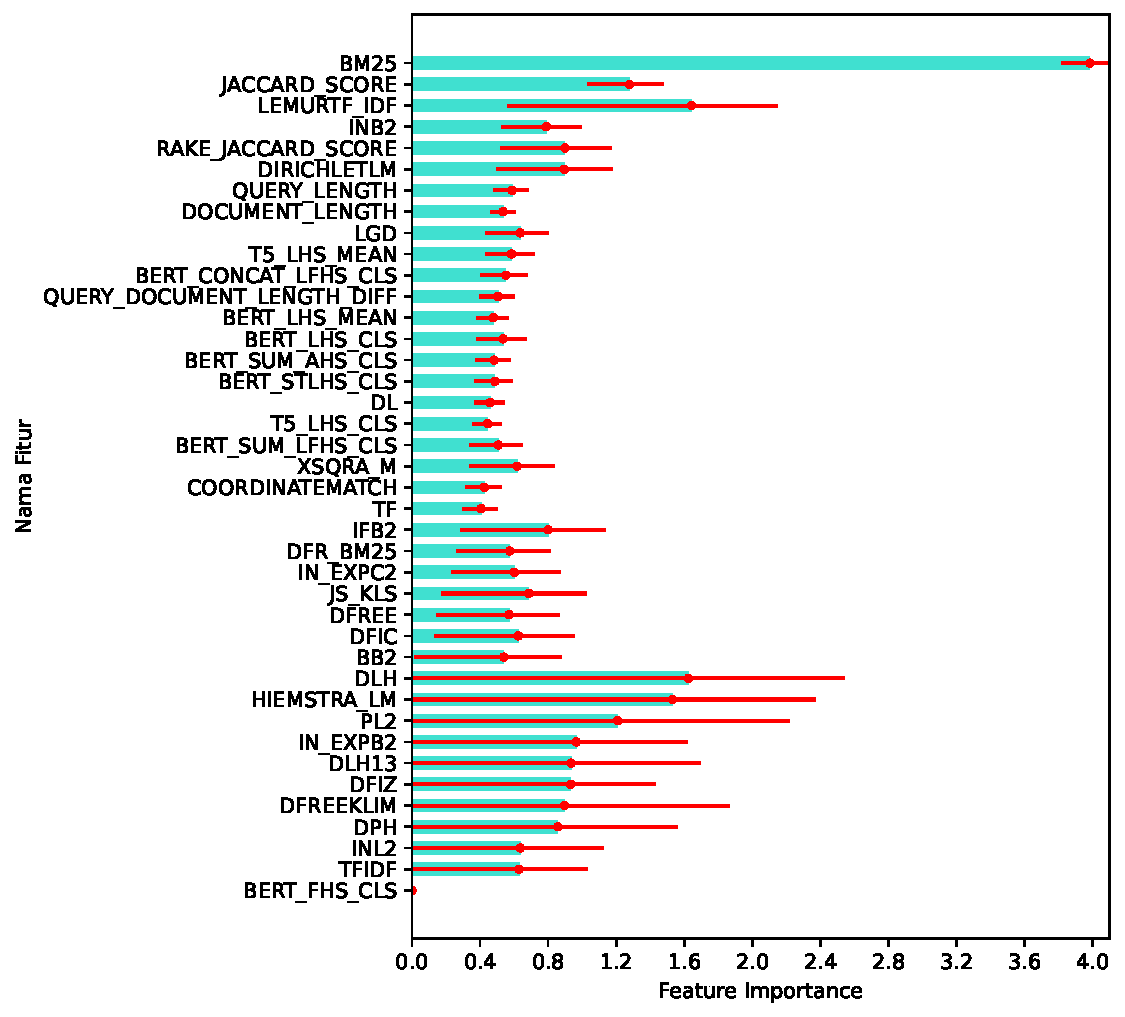
\includegraphics[scale=0.725]{assets/pdfs/Feature Importance Distribution Log.pdf}
    \caption{\Feature{} \importance{} ($fi$) secara umum, hasil agregasi kelima model dari seluruh \textit{fold}. Perhatikan bahwa sumbu-x merupakan nilai $fi$ dalam skala logaritmik dengan batang berwarna toska merupakan \textit{mean} $fi$ dan garis merah menunjukkan batas atas dan bawah distribusi $fi$ yang didapat dengan \textit{confidence interval} $95\%$. Sementara itu, sumbu-y merupakan daftar nama fitur yang diusulkan terurut secara menurun dari batas bawah distribusi terbesar atau yang diasumsikan paling konsisten.}
    \label{grafik:Feature Importance All}
\end{figure}
Perlu diketahui bahwa nilai dari \feature{} \importance{} $fi$ yang diperoleh berada dalam interval tertutup $fi\in[0,1]$ dengan nilai $fi=1$ berarti bahwa model hanya menggunakan satu fitur tersebut untuk melakukan seluruh \textit{split}, sedangkan $fi=0$ berarti bahwa fitur tersebut sama sekali tidak digunakan dalam pembuatan \textit{split}. Namun, sebelum divisualisasikan, karena nilai $fi$ yang diperoleh  sangat \textit{skew} maka dilakukan normalisasi terlebih dahulu dengan menggunakan fungsi logaritma. Perhatikan bahwa, karena nilai $fi$ masuk dalam interval tertutup $[0,1]$, maka hasil normalisasi menggunakan fungsi logaritma akan membuat grafik semakin \textit{skew}. Untuk mencegah hal tersebut, ditetapkan konstanta pengali $100$ untuk merubah interval tersebut menjadi interval tertutup $[0,100]$ dan konstanta penambah 1 untuk memungkinkan pemetaan bilangan riil tidak negatif. Oleh karena itu, fungsi normalisasi nilai $fi$ yang digunakan untuk visualisasi tersebut dapat dirumuskan sebagai $\log(fi \times 100+1)$.

Berdasarkan hasil yang didapat, ditemukan bahwa, secara rata-rata, lima fitur yang paling bermanfaat secara terurut dari yang paling penting adalah \obm{}, LEMURTF\_IDF, DLH, HIEMSTRA\_LM, dan JACCARD\_SCORE. Namun, dari kelima fitur tersebut, dua diantaranya memiliki standar deviasi tinggi, yaitu DLH dan HIEMSTRA\_LM, hal tersebut mencerminkan bahwa dari semua model \lambdamart{} yang dilatih, kedua fitur tersebut tidak konsisten menjadi fitur yang paling penting. Sementara itu, fitur-fitur seperti \obm{}, LEMURTF\_IDF, dan JACCARD\_SCORE menunjukkan hasil yang lebih konsisten, memiliki nilai tertinggi untuk batas bawah distribusi dengan \textit{confidence level} $95\%$, pada semua model yang dilatih.

Kemudian, seperti yang telah diusulkan pada \subbab{}~\ref{subbab:3:Usulan Fitur}, digunakan juga fitur-fitur yang memanfaatkan keluaran \encoder{}. Untuk metode pemanfaatan vektor \encoder{} \bert{}, ditemukan bahwa CONCAT\_LFHS\_CLS, sama dengan temuan \citet{devlin2018bert}, merupakan fitur yang paling efektif dalam melakukan klasifikasi menurut rata-rata nilai \importance{}-nya yang relatif lebih tinggi dibanding metode pemanfaatan vektor \bert{} lainnya. Selain itu, untuk metode pengambilan lainnya, ditemukan bahwa urutan nilai \importance{} yang didapat sama dengan urutan efektivitas temuan \citet{devlin2018bert}, dengan pengecualian LHS\_CLS. Hasil eksperimen menunjukkan bahwa LHS\_CLS merupakan fitur kedua yang paling efektif diantara metode pengambilan vektor \bert{} lainnya, bertentangan dengan \citet{devlin2018bert} yang mendapatkan LHS\_CLS sebagai metode terburuk kedua. Sementara itu, untuk metode pemanfaatan \encoder{} \tfive{} didapatkan bahwa hasil eksperimen sesuai dengan temuan \citet{ni2021sentence} dengan LHS\_MEAN sebagai fitur paling efektif. Dari semua metode pengambilan vektor yang diuji, didapat bahwa penggunaan LHS\_MEAN \encoder{} \tfive{} merupakan yang paling efektif, namun nilai \importance{}-nya masih lebih rendah dibandingkan algoritma pencocokan seperti JACCARD\_SCORE.

Berdasarkan hasil analisis \feature{} \importance{} tersebut, dilakukan pengujian efektivitas menggunakan data \testing{}. Dibentuk sistem yang sama dengan perbedaan pada jumlah fitur yang diekstraksi, yaitu dengan hanya mengekstraksi tiga fitur yang memiliki nilai $fi$ paling konsisten, antara lain nilai relevansi \obm{}, nilai relevansi LemurTF\_IDF, dan nilai kesamaan jaccard. Hasil percobaan tersebut diberikan pada \tabel{}~\ref{tabel:hasil test 3 fitur}. Menurut hasil percobaan, didapatkan bahwa, untuk metrik tolok ukur utama \recall{}$@3$, kinerja sistem relatif naik dengan penambahan proses \reranking{} menggunakan ketiga fitur tersebut. Selain metrik \recall{}$@3$, ditemukan juga peningkatan pada metrik \precision{}$@3$ yang mengindikasikan bahwa \reranking{} yang dilakukan dapat meningkatkan kualitas tiga dokumen teratas secara efektif.
\begin{table}[H]
    \centering
    \caption{Hasil eksperimen pada data \testing{} menggunakan \reranker{} dengan masukan nilai relevansi \obm{} dan LemurTF\_IDF, serta JACCARD\_SCORE yang diurutkan berdasarkan metrik \recall{}@3}
    \label{tabel:hasil test 3 fitur}
    \resizebox{\textwidth}{!}{%
        \begin{tabular}{lrrrrrrrrr}
	\toprule
	name & R@3 & R@5 & R@10 & recip\_rank & P@3 & P@5 & P@10 & map & nDCG@5 \\
	\midrule
	DLH13 (Reranker) & \textbf{0,7277} & 0,7723 & \underline{0,8614} & 0,7093 & \textbf{0,2871} & 0,1881 & \underline{0,1059} & 0,6613 & 0,6884 \\
	TF\_IDF (Reranker) & \underline{0,7228} & 0,7673 & \underline{0,8614} & 0,7101 & \underline{0,2838} & 0,1861 & \underline{0,1059} & 0,6585 & 0,6839 \\
	BM25 (Reranker) & 0,7129 & \underline{0,7871} & \textbf{0,8663} & 0,7036 & 0,2805 & \textbf{0,1921} & \textbf{0,1069} & 0,6574 & 0,6898 \\
	DLH13 & 0,7129 & \underline{0,7871} & \underline{0,8614} & \textbf{0,7345} & \underline{0,2838} & \underline{0,1901} & \underline{0,1059} & \textbf{0,6813} & \textbf{0,7082} \\
	InL2 (Reranker) & 0,7129 & 0,7822 & 0,8515 & 0,7040 & 0,2805 & 0,1881 & 0,1040 & 0,6561 & 0,6874 \\
	DFR\_BM25 (Reranker) & 0,7079 & \textbf{0,7921} & \textbf{0,8663} & 0,6995 & 0,2772 & \textbf{0,1921} & \textbf{0,1069} & 0,6521 & 0,6880 \\
	BM25 & 0,6881 & \underline{0,7871} & \underline{0,8614} & 0,7147 & 0,2739 & \underline{0,1901} & \underline{0,1059} & 0,6568 & 0,6919 \\
	InL2 & 0,6881 & \underline{0,7871} & \underline{0,8614} & \underline{0,7201} & 0,2706 & \underline{0,1901} & \underline{0,1059} & \underline{0,6693} & \underline{0,6997} \\
	TF\_IDF & 0,6881 & \underline{0,7871} & \underline{0,8614} & 0,7200 & 0,2706 & \underline{0,1901} & \underline{0,1059} & 0,6652 & 0,6975 \\
	DFR\_BM25 & 0,6782 & \underline{0,7871} & 0,8564 & 0,7126 & 0,2706 & \underline{0,1901} & 0,1050 & 0,6573 & 0,6919 \\
	\bottomrule
	\end{tabular}%
    }
\end{table}

Namun, kasus yang sama tidak bisa digeneralisasikan untuk metrik lainnya, seperti yang didapatkan bahwa terjadi penurunan kinerja sistem menurut beberapa metrik. Perubahan nilai metrik diberikan dalam \tabel{}~\ref{tabel:hasil test persentase kenaikan}. Perhatikan bahwa, walaupun didapatkan peningkatan pada \recall{}$@3$, terdapat beberapa penurunan nilai metrik untuk \recall{}$@5$ atau \recall{}$@10$. Hal tersebut menunjukkan bahwa, secara rata-rata, penambahan \reranker{} dengan tiga fitur tersebut dapat meningkatkan kemampuan sistem untuk mengidentifikasi dokumen relevan pada tiga hasil teratas. Tetapi, selain tiga hasil teratas, relevansi yang didapatkan kurang lebih sama atau bahkan menurun, yang berarti sistem tidak efektif dalam mempertahankan relevansi untuk cakupan yang lebih luas. Hal yang serupa dapat ditemukan pada metrik \precision{} dengan kenaikan pada \precision{}$@3$ dan beberapa penurunan atau stagnasi pada \precision{}$@5$ maupun \precision{}$@10$.

\begin{table}[H]
    \centering
    \caption{Persentase perubahan metrik pada data \testing{}}
    \label{tabel:hasil test persentase kenaikan}
    \resizebox{\textwidth}{!}{%
        \begin{tabular}{lrrrrrrrrr}
	\toprule
	name & R@3 & R@5 & R@10 & recip\_rank & P@3 & P@5 & P@10 & map & nDCG@5 \\
	\midrule
	TF\_IDF (Reranker) & \textbf{5,036}\% & -2,516\% & 0,000\% & \textbf{-1,375}\% & \textbf{4,878}\% & -2,083\% & 0,000\% & -1,000\% & -1,950\% \\
	DFR\_BM25 (Reranker) & \underline{4,380}\% & \textbf{0,629}\% & \textbf{1,156}\% & -1,850\% & 2,439\% & \textbf{1,042}\% & \textbf{1,887}\% & \underline{-0,793}\% & \underline{-0,575}\% \\
	BM25 (Reranker) & 3,597\% & \underline{0,000}\% & \underline{0,575}\% & \underline{-1,553}\% & 2,410\% & \textbf{1,042}\% & \underline{0,935}\% & \textbf{0,095}\% & \textbf{-0,299}\% \\
	InL2 (Reranker) & 3,597\% & -0,629\% & -1,149\% & -2,226\% & \underline{3,659}\% & \underline{-1,042}\% & -1,869\% & -1,963\% & -1,767\% \\
	DLH13 (Reranker) & 2,083\% & -1,887\% & 0,000\% & -3,439\% & 1,163\% & \underline{-1,042}\% & 0,000\% & -2,929\% & -2,800\% \\
        \hline
        \textit{mean} & 3,739\% & -0,881\% & 0,116\% & -2,089\% & 2,910\% & -0,417\% & 0,190\% & -1,318\% & -1,478\% \\
	\bottomrule
	\end{tabular}%
    }
\end{table}

Sama seperti analisis sebelumnya, dilakukan perhitungan \textit{t-test} untuk mendapatkan signifikansi dari dampak tersebut. Dapat dilihat pada \tabel{}~\ref{tabel:hasil test ttest} yang menunjukkan nilai \textit{p-value} untuk setiap metrik yang diperoleh pada pengujian menggunakan data \testing{}. Menurut hasil tersebut, penambahan proses \reranking{} yang memanfaatkan \reranker{} berbasis fitur dengan tiga fitur masukan tersebut tidak memiliki dampak signifikan untuk setiap metrik. Oleh karena itu, menurut metrik utama \recall{}$@3$, dapat disimpulkan bahwa \reranking{} menggunakan ketiga fitur tersebut dapat meningkatkan performa sistem \ir{} sekitar $3,739\%$ namun tidak cukup signifikan.
\begin{table}[H]
    \centering
    \caption{Hasil \textit{t-test} eksperimen pada data \testing{}}
    \label{tabel:hasil test ttest}
    \resizebox{\textwidth}{!}{%
        \begin{tabular}{lrrrrrrrrr}
	\toprule
        \multirow{2}{*}{name} & \multicolumn{9}{c}{\textit{p-value}} \\ \cline{2-10}
        & R@3 & R@5 & R@10 & recip\_rank  & P@3 & P@5 & P@10 & map & nDCG@5 \\
	\midrule
	BM25 (Reranker) & 0,4376 & 1,0000 & 0,7647 & 0,6433 & 0,5955 & 0,7831 & 0,6570 & 0,9777 & 0,9243 \\
	DFR\_BM25 (Reranker) & 0,3453 & 0,8737 & 0,6195 & 0,5879 & 0,6195 & 0,7977 & 0,5298 & 0,8197 & 0,8597 \\
	DLH13 (Reranker) & 0,5800 & 0,5925 & 1,0000 & 0,3101 & 0,7647 & 0,7831 & 1,0000 & 0,3733 & 0,3680 \\
	InL2 (Reranker) & 0,3557 & 0,8628 & 0,5298 & 0,5194 & 0,3683 & 0,7977 & 0,3197 & 0,5766 & 0,5839 \\
	TF\_IDF (Reranker) & 0,2248 & 0,4680 & 1,0000 & 0,6675 & 0,2502 & 0,5663 & 1,0000 & 0,7641 & 0,5357 \\
	\bottomrule
	\end{tabular}%
    }
\end{table}
%-----------------------------------------------------------------------------%





%-----------------------------------------------------------------------------%
\subsection{Hasil Pengaruh \Cutoff{}}
\label{subbab:5::Hasil Pengaruh Cut-off}
Perlu diingat bahwa, dalam penelitian ini, performa sistem akan diukur menggunakan metrik \recall{}$@3$. \gambar{}~\ref{grafik:cutoff} memvisualisasikan performa sistem pada beberapa nilai \cutoff{}. Dapat dilihat bahwa sistem DLH13 (Reranker) memiliki hasil yang paling baik pada \cutoff{} 85, sedangkan efektivitas kedua terbaik didapatkan oleh sistem TF\_IDF pada \cutoff{} 150. Oleh karena itu, berdasarkan pengamatan nilai terbaik, kurang adanya bukti yang dapat mendukung hipotesis awal peneliti, yaitu terdapat korelasi positif antara nilai \cutoff{} dengan kinerja sistem.

\begin{landscape}
    \begin{figure}
        \centering
        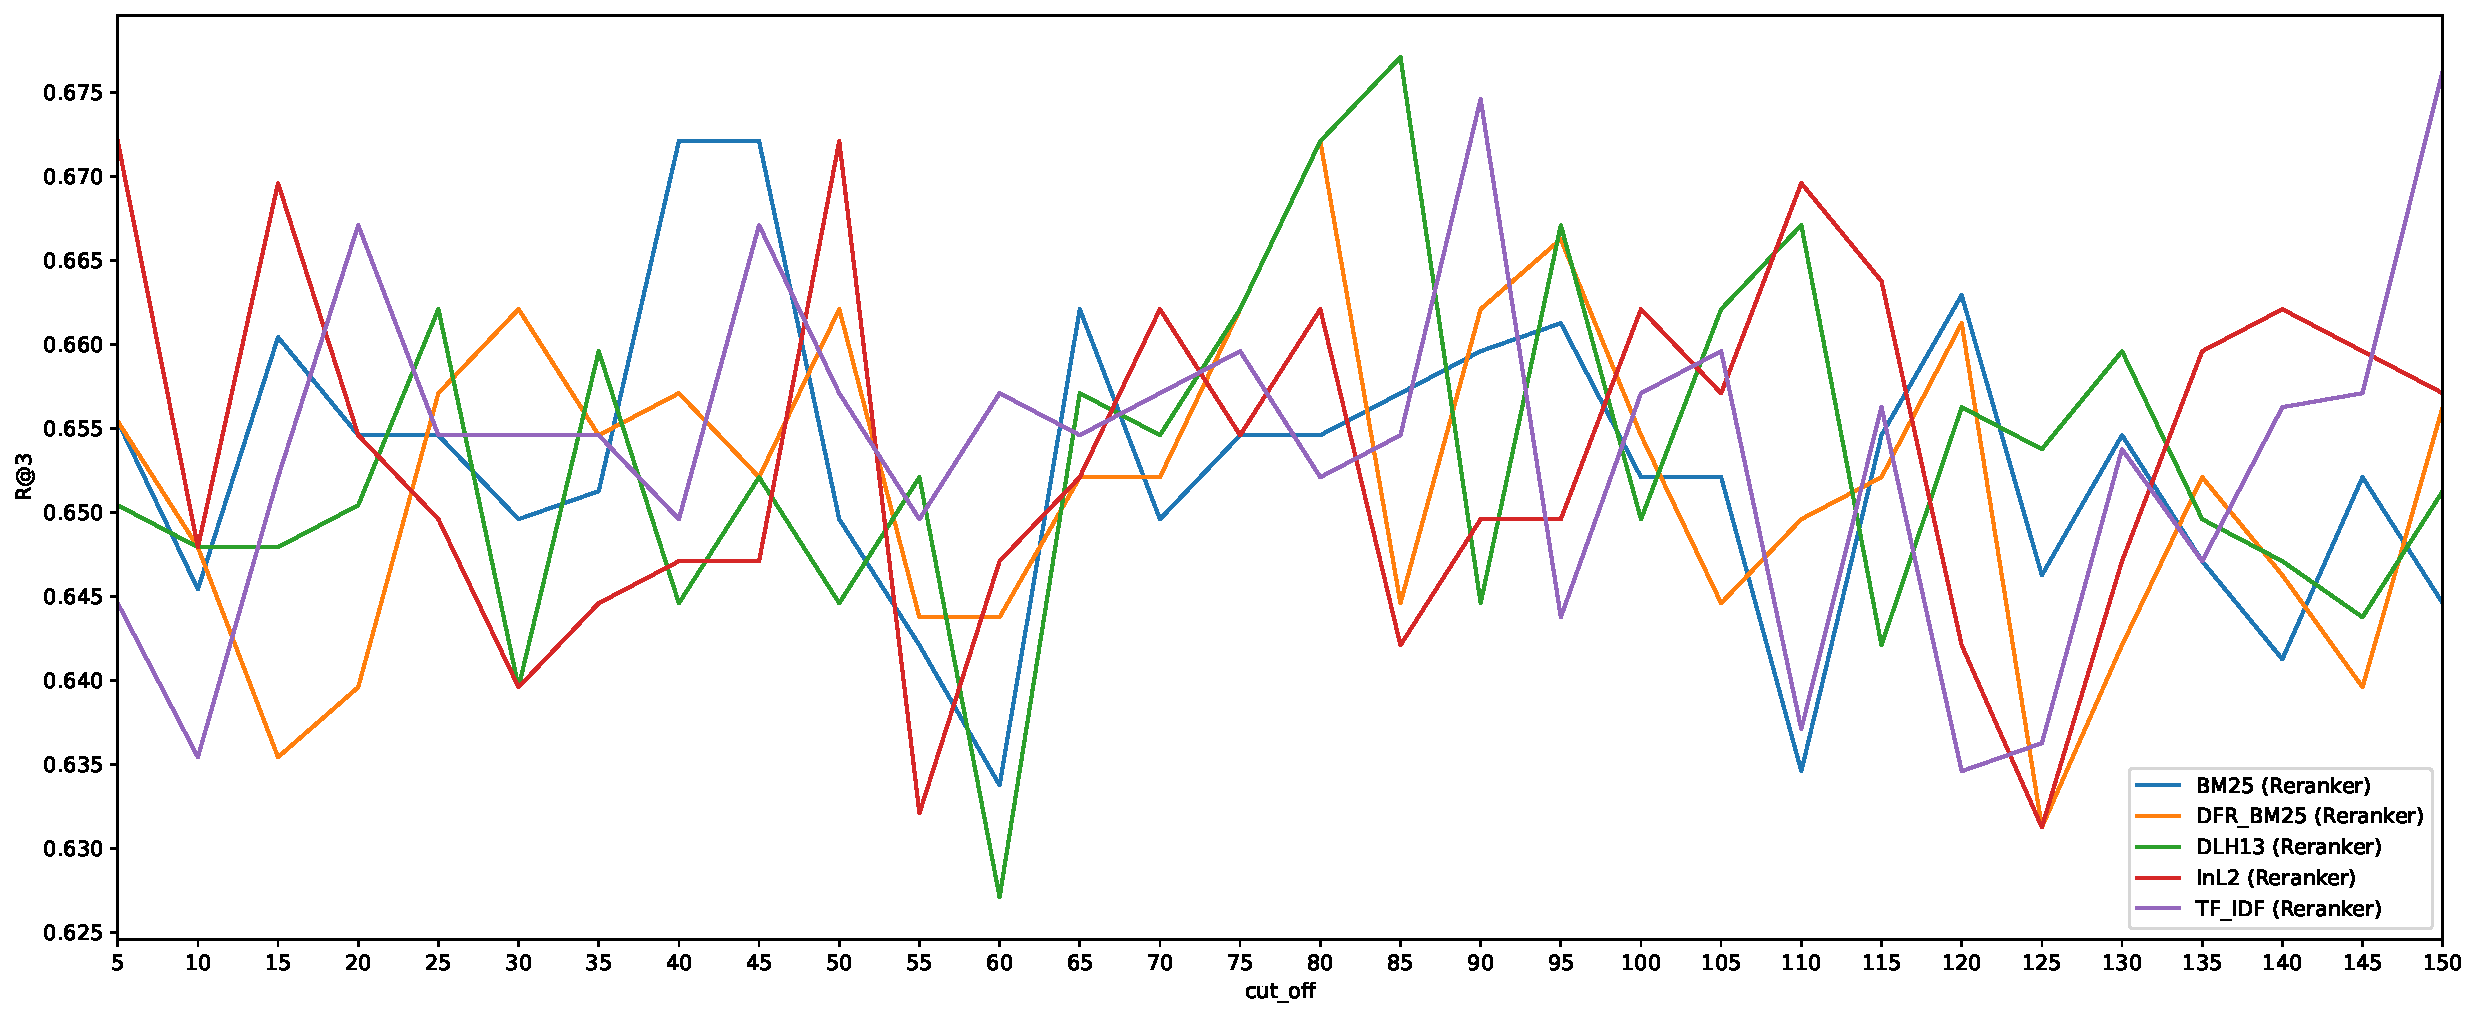
\includegraphics[scale=0.6]{assets/pdfs/Cut Off Experiment Results_3.pdf}
        \caption{Kinerja pada beberapa \cutoff{}. Perhatikan bahwa tidak didapatkannya korelasi yang kuat dengan nilai \textit{pearson} sebagai berikut: BM25 (Reranker) -0.2363; DFR\_BM25 (Reranker) -0.0904; DLH13 (Reranker) 0.1239; InL2 (Reranker) 0.0277; dan TF\_IDF (Reranker) 0.046. Hasil tersebut menunjukkan bahwa BM25 (Reranker) memiliki korelasi negatif yang sangat lemah dan DFR\_BM25 (Reranker) memiliki korelasi negatif yang lemah, serta DLH13 (Reranker), InL2 (Reranker), dan TF\_IDF (Reranker) memiliki korelasi positif yang lemah.}
        \label{grafik:cutoff}
    \end{figure}
\end{landscape}

Selain dari itu, grafik tersebut kurang dapat menunjukkan korelasi antara \cutoff{} dengan efektivitas, sehingga, untuk menyelidiki hubungan tersebut, dilakukan perhitungan korelasi \textit{pearson} yang hasilnya dapat dilihat pada \gambar{}~\ref{grafik:cutoff}. Menurut hasil perhitungan tersebut, nilai mutlak tertinggi diperoleh BM25 (Reranker), senilai $0.2363$, yang tergolong tingkat korelasi lemah. Golongan korelasi itu juga merupakan korelasi negatif yang juga bertentangan dengan hipotesis awal peneliti, yaitu adanya korelasi positif.

Selanjutnya, dilakukan analisis distribusi \ranking{} dari dokumen relevan karena peneliti menduga bahwa model \lambdamart{} kurang efektif dalam memperbaiki \ranking{} untuk posisi yang rendah. Untuk itu, dilakukan perbandingan distribusi sebelum dan setelah proses \reranking{} yang hasilnya divisualisasikan pada \gambar{}~\ref{grafik:dist rank}. Perlu diketahui bahwa grafik tersebut merupakan hasil \textit{Kernel Density Estimation} (KDE) yang digunakan untuk menghasilkan suatu kurva kontinu dari himpunan data diskret. Dalam kasus ini, data diskret tersebut merupakan nilai peringkat atau \textit{rank} yang memiliki rentang nilai $[1,\infty)$ dengan peringkat $1$ merupakan peringkat tertinggi. Dapat dilihat bahwa dugaan peneliti salah mengenai efektivitas model pada peringkat rendah karena model \lambdamart{} berhasil memperbaiki \ranking{} bahkan untuk posisi lebih dari $80$. Hal tersebut juga dapat ditemukan pada sistem keempat sistem lainnya. Oleh karena itu, peneliti menyimpulkan beberapa faktor yang dapat menyebabkan tidak diperolehnya korelasi positif antara \recall{}$@3$ dan \cutoff{}, antara lain fitur yang kurang dapat menangkap karakteristik pasangan kueri-dokumen yang juga merupakan eksperimen utama penelitian ini, model atau arsitektur yang kurang kompleks, atau terjadinya \textit{overfitting}.
\begin{figure}[!ht]
    \centering
    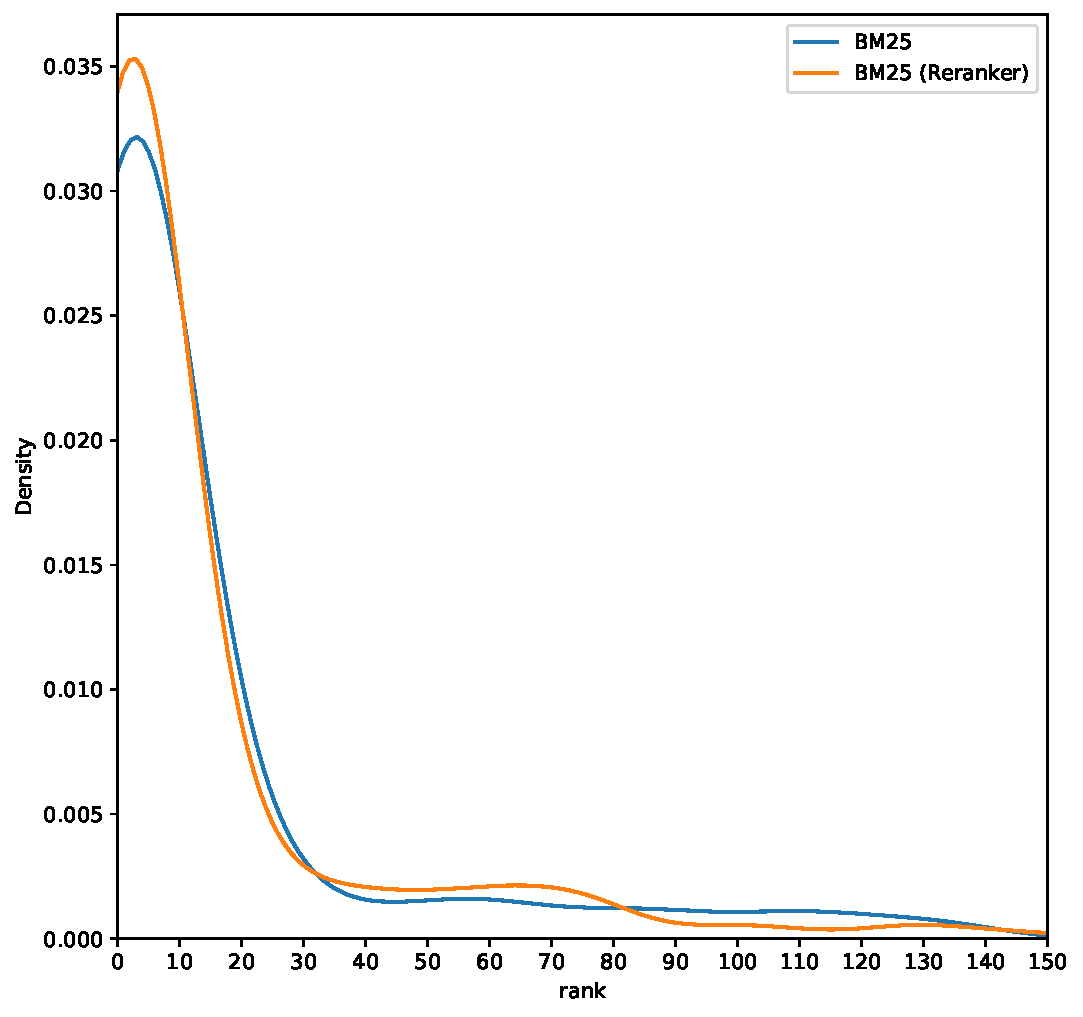
\includegraphics[scale=0.6]{assets/pdfs/Rank KDE BM25.pdf}
    \caption{Distribusi peringkat (\textit{rank}) untuk sistem dengan tahap \ranking{} pertama \obm{}. Perhatikan bahwa sumbu-x (\textit{rank}) adalah peringkat yang diperoleh suatu kueri setelah melakukan proses \retrieval{} dan sumbu-y merupakan nilai estimasi kurva distribusi \textit{rank} dengan menggunakan KDE.}
    \label{grafik:dist rank}
\end{figure}
%-----------------------------------------------------------------------------%





%-----------------------------------------------------------------------------%
\section{Rangkuman Hasil Eksperimen}
\label{subbab:5:Rangkuman Hasil Eksperimen}
% \todo{FEATURE IMPORTANCE BEST ONES\\FEATURE IMPORTANCE ENCODER EMBEDDING X CHK\\PERFORMANCE VAL\\SIGNIFICANCE VAL\\PERFORMANCE TEST WITH SELECTED FEATURES\\SIGNIFICANCE TEST WITH SELECTED FEATURES\\CUT-OFF CORRELATION\\HYPOTHESIS CORRELATION}

Berdasarkan hasil eksperimen, didapat bahwa penambahan \lambdamart{} sebagai \reranker{} dengan menggunakan seluruh fitur usulan dapat mengingkatkan seluruh metrik sekitar $4,17\%$ dan $4,19\%$ untuk metrik utama secara signifikan. Terdapat tiga sistem yang ditemukan memiliki performa terbaik berdasarkan kasus tertentu. Pertama, DLH13 (Reranker) merupakan sistem terbaik untuk melakukan pengembalian dokumen pada 3 hasil teratas yang diindikasikan dengan metrik \recall{}$@3$ dan \precision{}$@3$ tertinggi diantara kelima sistem tersebut. Namun, untuk cakupan dokumen yang lebih luas, TF\_IDF (Reranker) dapat dijadikan alternatif karena mendapatkan metrik \recall{}$@10$ dan \precision{}$@10$ tertinggi dibandingkan sistem lainnya. Sementara itu, DFR\_BM25 (Reranker) merupakan hasil yang baik dibandingkan dengan sistem lainnya dalam kasus tertentu yang memerlukan ketepatan pengembalian pada dokumen-dokumen teratas dibandingkan jumlah relevansi yang dikembalikan.

Kemudian, dari hasil analisis \feature{} \importance{}, terdapat tiga fitur yang penting untuk melakukan penilaian relevansi dokumen, yaitu nilai relevansi dari \obm{} dan LEMURTF\_IDF, serta nilai kesamaan jaccard antara himpunan kata dokumen dan kueri. Dengan hanya ketiga fitur tersebut, diuji performa sistem pada data \testing{}. Hasil menunjukkan peningkatan pada \recall{}$@3$ dan \precision{}$@3$, namun tidak sepenuhnya membaik untuk metrik lainnya. Oleh karena itu, dapat disimpulkan bahwa, berdasarkan metrik utama, ketiga fitur tersebut dapat meningkatkan kinerja sekitar $3,739\%$ namun belum cukup signifikan. Selain itu, ditemukan bahwa \importance{} fitur \encoder{} serupa dengan performa temuan penelitian sebelumnya~\citep{devlin2018bert, ni2021sentence}, namun kurang bermanfaat untuk menentukan relevansi dokumen legal, melihat bahwa fitur tersebut memiliki \importance{} yang lebih kecil dibandingkan perhitungan kesamaan sederhana seperti jaccard.

Sementara itu, berdasarkan pengamatan, tidak ditemukan korelasi antara \cutoff{} dan efektivitas untuk rentang \cutoff{} dari 5 sampai 150 dengan interval 5. Namun, menurut nilai perhitungan korelasi \textit{pearson}, ditemukan korelasi positif sangat lemah untuk sistem DLH13 (Reranker), InL2 (Reranker), dan TF\_IDF (Reranker). Sementara itu, terdapat korelasi negatif lemah untuk sistem DFR\_BM25 (Reranker) dan korelasi negatif sangat lemah untuk sistem BM25 (Reranker). Hal tersebut bertentangan dengan hipotesis awal bahwa semakin banyak dokumen yang dikembalikan maka \lambdamart{} dapat melakukan lebih banyak pertimbangan yang dapat semakin meningkatkan kinerja sistem.
%-----------------------------------------------------------------------------%





%-----------------------------------------------------------------------------%
% \begin{figure}
%     \centering
%     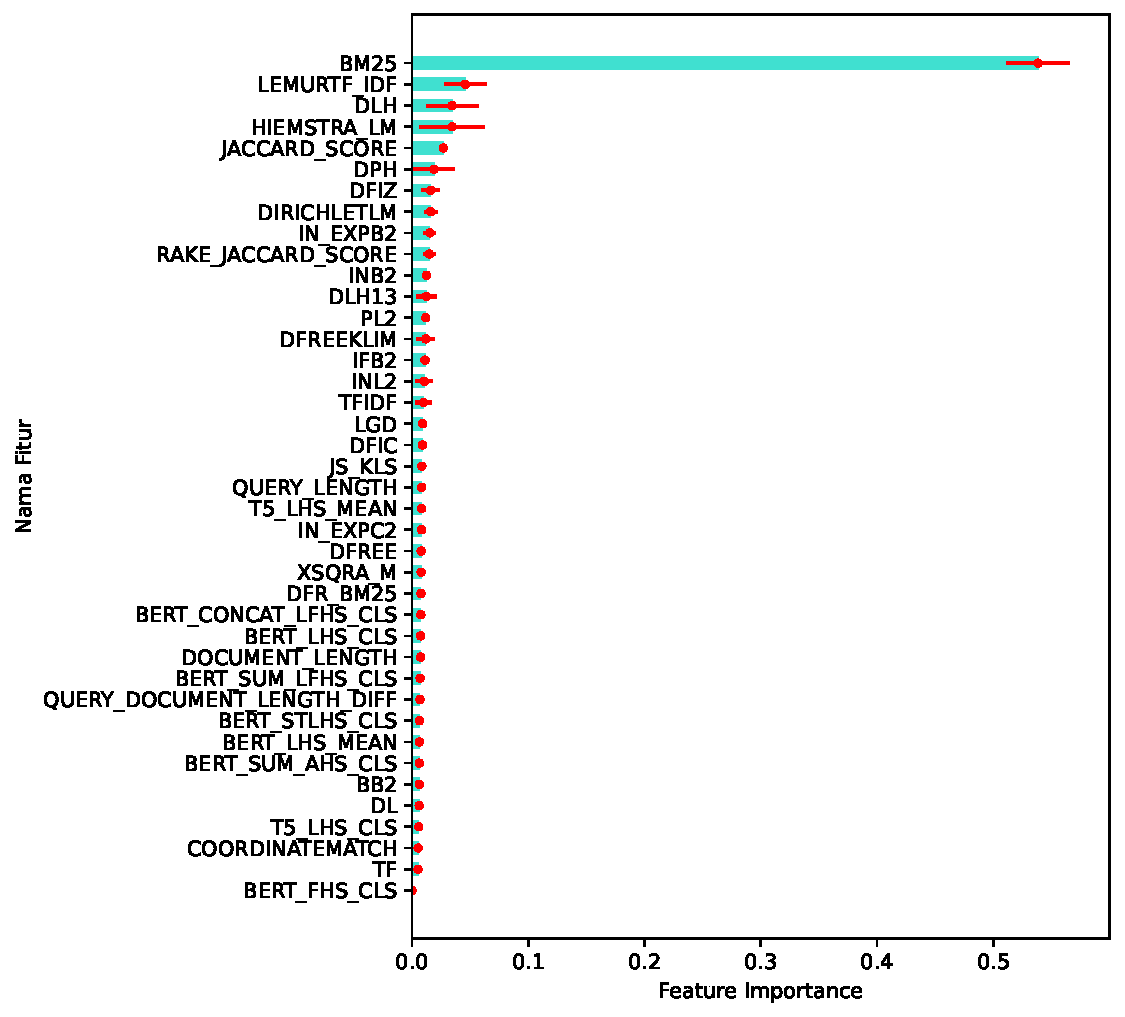
\includegraphics[scale=0.65]{assets/pdfs/Feature Importance BM25.pdf}
%     \caption{Feature Importance BM25 (Reranker)}
%     \label{grafik:Feature Importance BM25 All}
% \end{figure}

% \begin{figure}
%     \centering
%     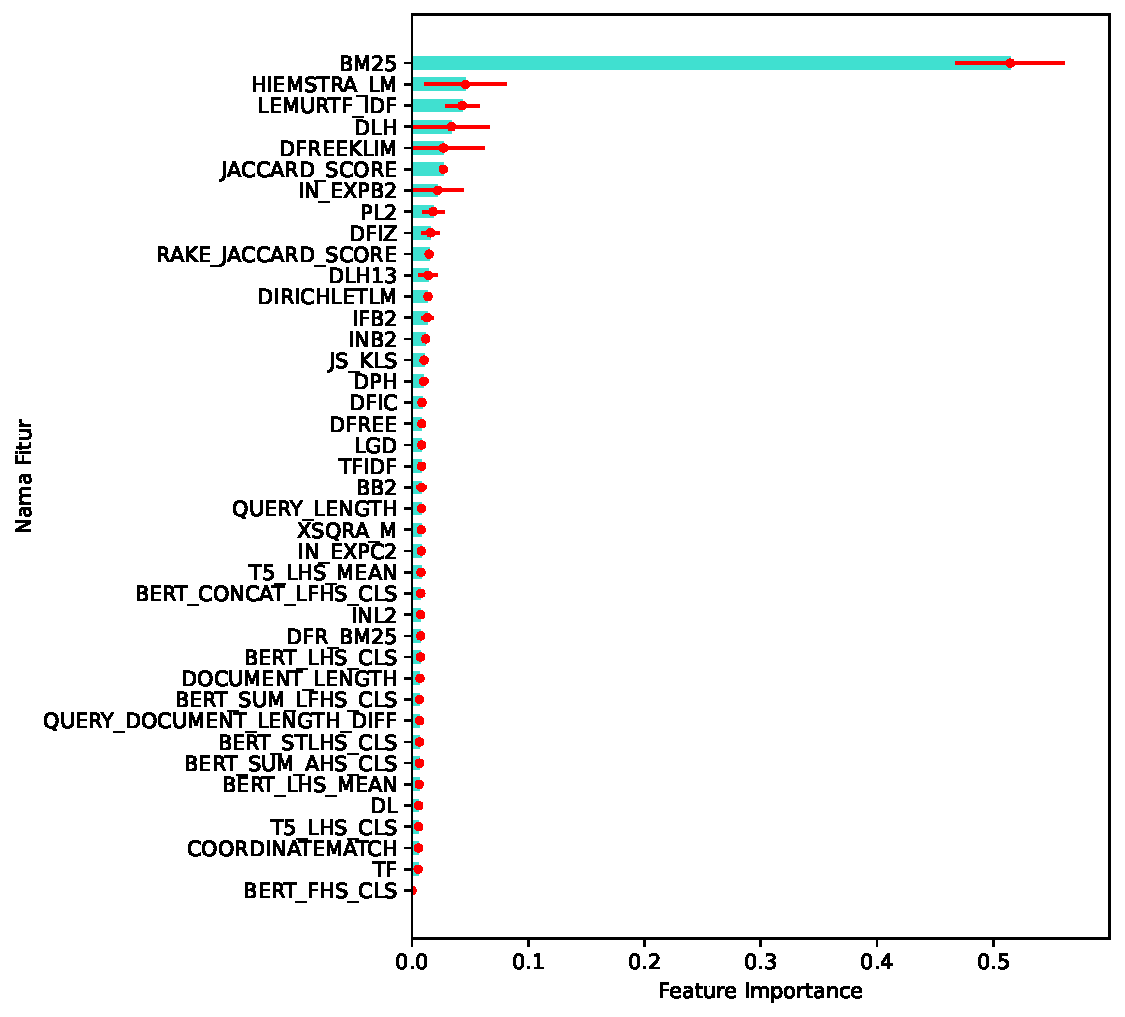
\includegraphics[scale=0.65]{assets/pdfs/Feature Importance TF_IDF.pdf}
%     \caption{Feature Importance TF\_IDF (Reranker)}
%     \label{grafik:Feature Importance TF_IDF All}
% \end{figure}

% \begin{figure}
%     \centering
%     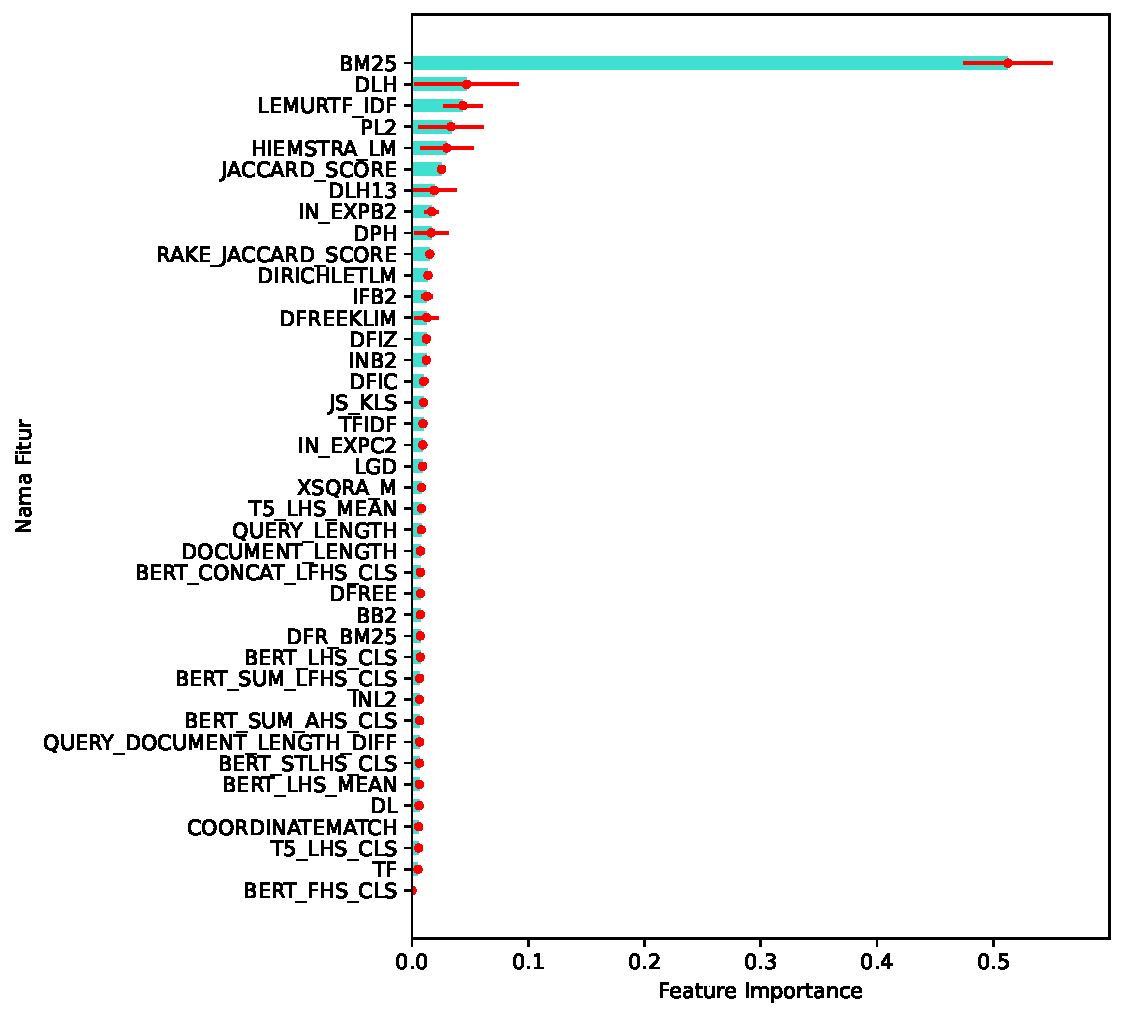
\includegraphics[scale=0.65]{assets/pdfs/Feature Importance InL2.pdf}
%     \caption{Feature Importance InL2 (Reranker)}
%     \label{grafik:Feature Importance InL2 All}
% \end{figure}

% \begin{figure}
%     \centering
%     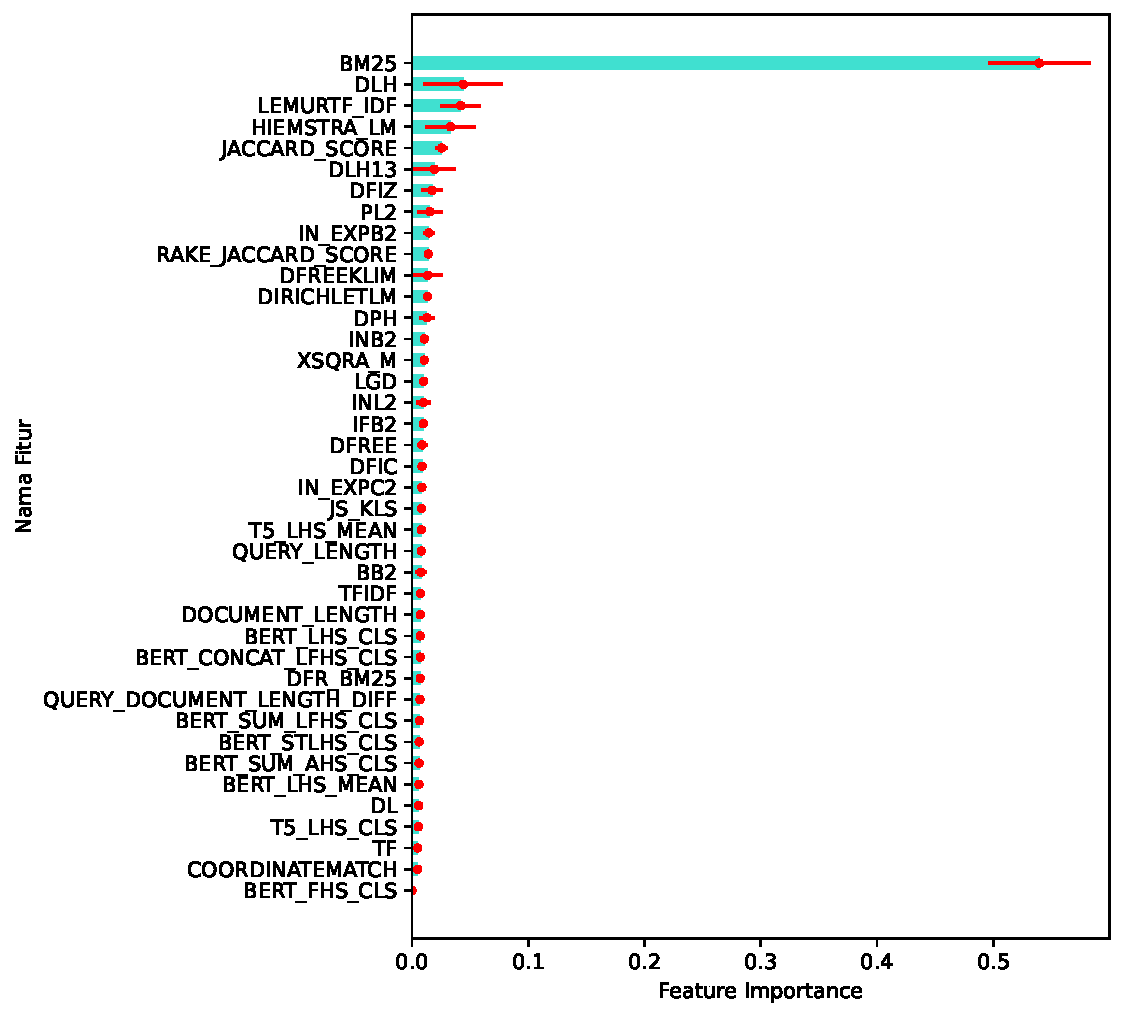
\includegraphics[scale=0.65]{assets/pdfs/Feature Importance DFR_BM25.pdf}
%     \caption{Feature Importance DFR\_BM25 (Reranker)}
%     \label{grafik:Feature Importance DFR_BM25 All}
% \end{figure}

% \begin{figure}
%     \centering
%     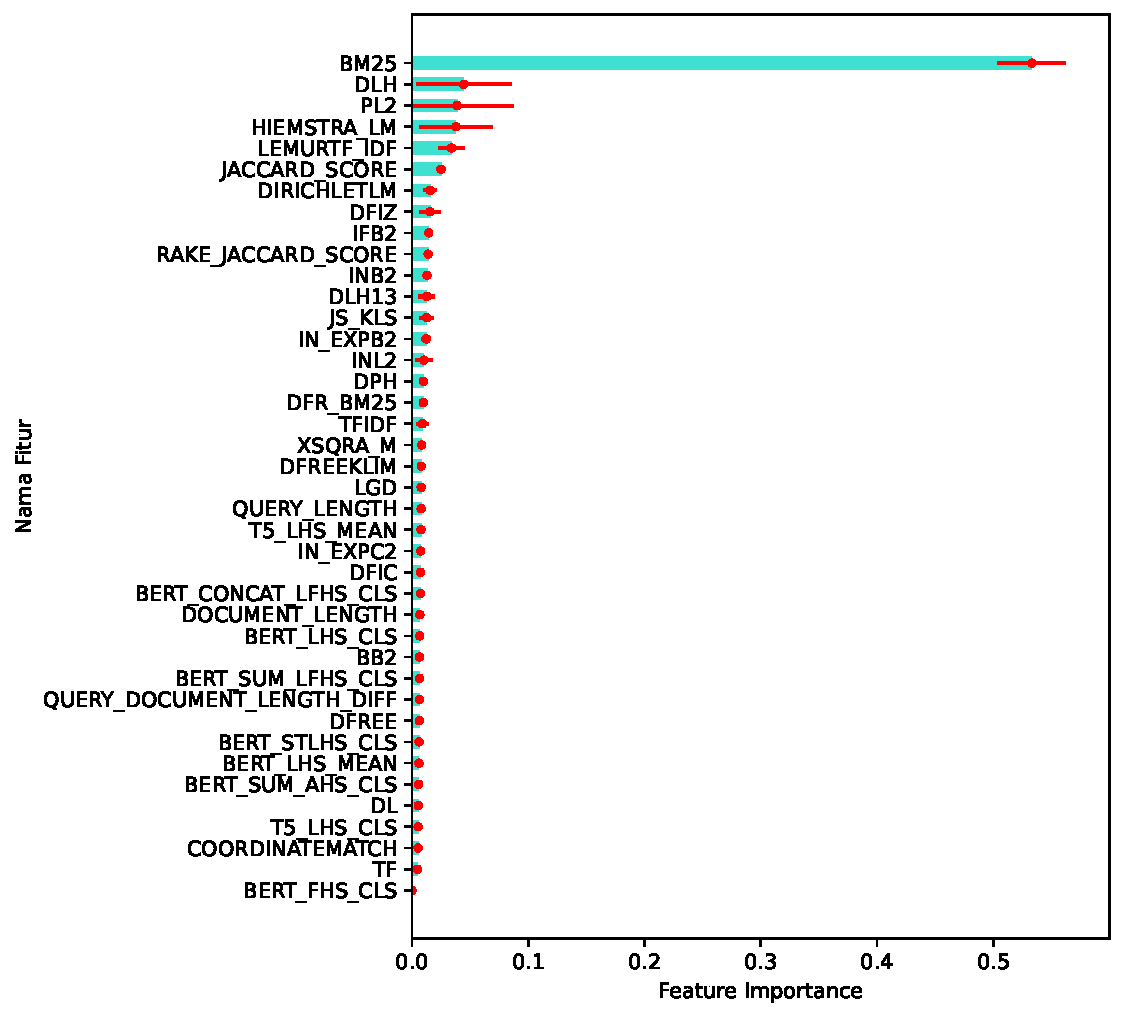
\includegraphics[scale=0.65]{assets/pdfs/Feature Importance DLH13.pdf}
%     \caption{Feature Importance DLH13 (Reranker)}
%     \label{grafik:Feature Importance DLH13 All}
% \end{figure}
%-----------------------------------------------------------------------------%
\clearchapter
%---------------------------------------------------------------
\chapter{\babEnam}
\label{bab:6}
Setelah melakukan eksperimen dan analisis hasil, pada \bab{}~\ref{bab:6} akan dipaparkan kesimpulan penelitian dan saran penelitian berikutnya. Pada \subbab{}~\ref{subbab:kesimpulan} ditarik kesimpulan dari analisis yang telah dilakukan. Kemudian, \subbab{}~\ref{subbab:saran} membahas tentang saran untuk penelitian berikutnya.
%---------------------------------------------------------------





%---------------------------------------------------------------
\section{Kesimpulan}
\label{subbab:kesimpulan}
\subbab{} ini menyajikan kesimpulan utama dari penelitian yang telah dilakukan. Berdasarkan analisis dan hasil eksperimen, beberapa poin penting dapat disimpulkan sebagai berikut:

\vspace{2mm}
\noindent\textbf{Karakteristik Fitur}. Menurut hasil eksperimen yang didapatkan, karakteristik yang dapat membedakan jenis relevansi adalah fitur nilai relevansi \obm{}, relevansi LEMURTF\_IDF, dan kesamaan jaccard. Ketiga fitur tersebut secara konsisten mendapatkan nilai \textit{feature importance} yang tinggi dari seluruh sistem yang diuji.

\vspace{2mm}
\noindent\textbf{Peningkatan Efektivitas}. Pemanfaatan seluruh fitur untuk \reranking{} dapat meningkatkan performa seluruh metrik sekitar $4,17\%$ secara signifikan. Sedangkan pemanfaatan himpunan bagian dari fitur yang diusulkan, yaitu ketiga fitur terpenting yang konsisten, dapat meningkatkan nilai metrik utama sekitar $3, 739\%$, namun tidak cukup signifikan saat diuji menggunakan data \testing{}.
% \begin{itemize}
%     \item Pemanfaatan seluruh fitur untuk \reranking{} dapat meningkatkan performa seluruh metrik sekitar $4,17\%$ secara signifikan;
%     \item Fitur nilai relevansi \obm{}, relevansi LEMURTF\_IDF, dan kesamaan jaccard merupakan karakteristik penting dari pasangan pertanyaan-pasal untuk melakukan penilaian relevansi;
%     \item Fitur nilai relevansi \obm{}, relevansi LEMURTF\_IDF, dan kesamaan jaccard dapat meningkatkan performa sistem sekitar $3, 739\%$ namun tidak cukup signifikan saat diuji menggunakan data \testing{};
%     \item Hasil kinerja \base{} \retriever{} tidak dapat dipastikan memiliki peningkatan efektivitas yang setara dengan ditambahkannya \reranker{} berbasis fitur walaupun menggunakan himpunan fitur yang sama;
%     \item Kinerja terbaik untuk \recall{} pada \cutoff{} 3, secara umum, didapatkan menggunakan sistem \ir{} dengan DLH13 sebagai \base{} \retriever{} dan \reranker{} \lambdamart{} menggunakan seluruh fitur yang diusulkan;
%     \item Tidak ditemukan korelasi yang kuat antara nilai \cutoff{} dan efektivitas dari sistem \cascaded{} \ir{} berdasarkan nilai korelasi \textit{pearson}.
% \end{itemize}
%---------------------------------------------------------------





%---------------------------------------------------------------
\section{Saran}
\label{subbab:saran}
Berdasarkan hasil penelitian ini, terdapat beberapa saran untuk penelitian selanjutnya:
\begin{itemize}
\item Replikasi metode yang telah diusulkan pada dokumen hukum berbahasa Indonesia;
\item Menginvestigasi jumlah fitur yang efisien untuk suatu himpunan fitur menggunakan \textit{incremental ablation learning};
\item Perlu dilakukan penelitian lebih lanjut untuk mengeksplorasi fitur-fitur tambahan yang dapat meningkatkan efektivitas klasifikasi relevansi. Penggunaan teknik pembelajaran mesin yang lebih canggih, seperti \textit{deep learning}, juga patut dipertimbangkan;
\item Penelitian mendalam terhadap kombinasi berbagai \reranker{} berbasis fitur perlu dilakukan untuk mengidentifikasi konfigurasi yang paling efektif dalam meningkatkan kinerja \retriever{};
\item Pengembangan dan pengujian model yang lebih kompleks untuk sistem \cascaded{} \ir{} dengan menambahkan tahapan \ranking{} untuk mengidentifikasi faktor-faktor yang berkontribusi terhadap efektivitas sistem;
\item Implementasi dan evaluasi metode pada skenario diluar domain legal untuk memberikan wawasan berharga mengenai kinerja sistem dalam lingkup yang beragam.
\end{itemize}
%---------------------------------------------------------------




%---------------------------------------------------------------
% Pada bab ini, Penulis akan memaparkan kesimpulan penelitian dan saran untuk penelitian berikutnya.
% \item Studi komprehensif tentang pengaruh berbagai metode \retriever{} dan \reranker{} terhadap \recall{} pada berbagai \cutoff{} akan memberikan pemahaman yang lebih baik mengenai dinamika sistem \ir{};


% %---------------------------------------------------------------
% \section{Kesimpulan}
% \label{subbab:kesimpulan}
% %---------------------------------------------------------------
% Berikut ini adalah kesimpulan terkait pekerjaan yang dilakukan dalam penelitian ini:
% \begin{enumerate}
% 	\item \bo{Poin pertama} \\
% 	Penjelasan poin pertama.
% 	\item \bo{Poin kedua} \\
% 	Penjelasan poin kedua.
% \end{enumerate}

% Tulis kalimat penutup di sini.


% %---------------------------------------------------------------
% \section{Saran}
% \label{subbab:saran}
% %---------------------------------------------------------------
% Berdasarkan hasil penelitian ini, berikut ini adalah saran untuk pengembangan penelitian berikutnya:
% \begin{enumerate}
% 	\item Saran 1.
% 	\item Saran 2.
% \end{enumerate}

\clearchapter

%
% Daftar Pustaka
\CAPinToC % All entries in ToC will be CAPITALIZED from here on
%
% Daftar Pustaka
%

%
% Tambahkan pustaka yang digunakan setelah perintah berikut.
%
\phantomsection %hack to add clickable section for pustaka
\bibliography{config/references}

\clearchapter
\noCAPinToC % Revert to original \addcontentsline formatting

%
% Lampiran
%
\begin{appendix}
	\newcounter{pagetemp}
	\setcounter{pagetemp}{\thepage}
	%
% @author  Andreas Febrian
% @version 1.00
%
% Hanya sebuah pembatas bertuliskan LAMPIRAN ditengah halaman.
%

\begin{titlepage}
\centering
\vspace*{6cm}
\noindent \Huge{LAMPIRAN}
\end{titlepage}

	\clearchapter
	\setcounter{page}{\thepagetemp}
	\stepcounter{page}
	% %-----------------------------------------------------------------------------%
% \addappendix{CHANGELOG}
% \chapter*{Lampiran 1: CHANGELOG}
% \label{appendix:changelog}
% %-----------------------------------------------------------------------------%
% \todo{Silakan hapus lampiran ini ketika Anda mulai menggunakan \f{template}.}

% \f{Template} versi terbaru bisa didapatkan di \url{https://gitlab.com/ichlaffterlalu/latex-skripsi-ui-2017}.
% Daftar perubahan pada \f{template} hingga versi ini:
% \begin{itemize}
% 	\item versi 1.0.3 (3 Desember 2010):
% 		\begin{itemize}
% 			\item \f{Template} Skripsi/Tesis sesuai ketentuan \f{formatting} tahun 2008.
% 			\item Bisa diakses di \url{https://github.com/edom/uistyle}.
% 		\end{itemize}
% 	\item versi 2.0.0 (29 Januari 2020):
% 		\begin{itemize}
% 			\item \f{Template} Skripsi/Tesis sesuai ketentuan \f{formatting} tahun 2017.
% 			\item Menggunakan BibTeX untuk sitasi, dengan format \f{default} sitasi IEEE.
% 			\item \f{Template} kini bisa ditambahkan kode sumber dengan \f{code highlighting} untuk bahasa pemrograman populer seperti Java atau Python.
% 		\end{itemize}
% 	\item versi 2.0.1 (8 Mei 2020):
% 		\begin{itemize}
% 			\item Menambahkan dan menyesuaikan tutorial dari versi 1.0.3, beserta cara kontribusi ke template.
% 		\end{itemize}
% 	\item versi 2.0.2 (14 September 2020):
% 		\begin{itemize}
% 			\item Versi ini merupakan hasil \f{feedback} dari peserta skripsi di lab \f{Reliable Software Engineering} (RSE) Fasilkom UI, semester genap 2019/2020.
% 			\item BibTeX kini menggunakan format sitasi APA secara \f{default}.
% 			\item Penambahan tutorial untuk \code{longtable}, agar tabel bisa lebih dari 1 halaman dan header muncul di setiap halaman.
% 			\item Menambahkan tutorial terkait penggunaan BibTeX dan konfigurasi \f{header}/\f{footer} untuk pencetakan bolak-balik.
% 			\item Label "Universitas Indonesia" kini berhasil muncul di halaman pertama tiap bab dan di bagian abstrak - daftar kode program.
% 			\item \f{Hyphenation} kini menggunakan \code{babel} Bahasa Indonesia. Aktivasi dilakukan di \code{hype-indonesia.tex}.
% 			\item Minor adjustment untuk konsistensi \f{license} dari template.
% 		\end{itemize}
% 	\item versi 2.0.3 (15 September 2020):
% 		\begin{itemize}
% 			\item Menambahkan kemampuan orientasi \f{landscape} beserta tutorialnya.
% 			\item \code{\bslash{}captionsource} telah diperbaiki agar bisa dipakai untuk \code{longtable}.
% 			\item Daftar lampiran kini telah tersedia, lampiran sudah tidak masuk daftar isi lagi.
% 			\item Nomor halaman pada lampiran dilanjutkan dari halaman terakhir konten (daftar referensi).
% 			\item Kini sudah bisa menambahkan daftar isi baru untuk jenis objek tertentu (custom), seperti: "Daftar Aturan Transformasi".
% 			Sudah termasuk mekanisme \f{captioning} dan tutorialnya.
% 			\item Perbaikan minor pada tutorial.
% 		\end{itemize}
% 	\item versi 2.1.0 (8 September 2021):
% 		\begin{itemize}
% 			\item Versi ini merupakan hasil \f{feedback} dari peserta skripsi dan tesis di lab \f{Reliable Software Engineering} (RSE) Fasilkom UI, semester genap 2020/2021.
% 			\item Minor edit: "Lembar Pengesahan", dsb. di daftar isi menjadi all caps.
% 			\item Experimental multi-language support (Chinese, Japanese, Korean).
% 			\item Support untuk justifikasi dan word-wrapping pada tabel.
% 			\item Penggunaan suffix "(sambungan)" untuk tabel lintas halaman. Tambahan support suffix untuk \code{\bslash{}captionsource}.
% 		\end{itemize}
% 	\item versi 2.1.1 (7 Februari 2022):
% 		\begin{itemize}
% 			\item Update struktur mengikuti fork template versi 1.0.3 di \url{https://github.com/rkkautsar/edom/ui-thesis-template}.
% 			\item Support untuk simbol matematis \code{amsfonts}.
% 			\item Kontribusi komunitas terkait improvement GitLab CI, atribusi, dan format sitasi APA bahasa Indonesia.
% 			\item Perbaikan tutorial berdasarkan perubahan terbaru pada versi 2.1.0 dan 2.1.1.
% 		\end{itemize}
% 	\item versi 2.1.2 (13 Agustus 2022):
% 		\begin{itemize}
% 			\item Modifikasi penamaan beberapa berkas.
% 			\item Perbaikan beberapa halaman depan (halaman persetujuan, halaman orisinalitas, dsb.).
% 			\item Support untuk lembar pengesahan yang berbeda dengan format standar, seperti Laporan Kerja Praktik dan Disertasi.
% 			\item Kontribusi komunitas terkait kesesuaian dengan format Tugas Akhir UI, kelengkapan dokumen, perbaikan format sitasi, dan \f{quality-of-life}.
% 			\item Perbaikan tutorial.
% 		\end{itemize}
% 	\item versi 2.1.3 (22 Februari 2023):
% 		\begin{itemize}
% 			\item Dukungan untuk format Tugas Akhir Kelompok di Fasilkom UI.
% 			\item Dukungan untuk format laporan Kampus Merdeka Mandiri di Fasilkom UI.
% 			\item Minor bugfix: Perbaikan kapitalisasi variabel.
% 			\item Quality-of-Life: Pengaturan kembali \code{config/settings.tex}.
% 			\item Tutorial untuk beberapa \f{use case}.
% 		\end{itemize}
% \end{itemize}

% %-----------------------------------------------------------------------------%
% \addappendix{Judul Lampiran 2}
% \chapter*{Lampiran 2: Judul Lampiran 2}
% \label{appendix:sample}
% %-----------------------------------------------------------------------------%
% Lampiran hadir untuk menampung hal-hal yang dapat menunjang pemahaman terkait tugas akhir, namun akan mengganggu \f{flow} bacaan sekiranya dimasukkan ke dalam bacaan.
% Lampiran bisa saja berisi data-data tambahan, analisis tambahan, penjelasan istilah, tahapan-tahapan antara yang bukan menjadi fokus utama, atau pranala menuju halaman luar yang penting.

% %-----------------------------------------------------------------------------%
% \section*{Subbab dari Lampiran 2}
% \label{appendix:sampleSubchap}
% %-----------------------------------------------------------------------------%
% \todo{Isi subbab ini sesuai keperluan Anda. Anda bisa membuat lebih dari satu judul lampiran, dan tentunya lebih dari satu subbab.}

\end{appendix}

\end{document}
